% System-level mapping of automotive applications onto zonal E/E architectures
% Build: cd paper && make   (pdflatex + bibtex; figures: make figures)
\documentclass[10pt,a4paper,twocolumn]{article}
\raggedbottom

% ---- fonts and text --------------------------------------------------------
\usepackage[T1]{fontenc}
\usepackage[utf8]{inputenc}
\usepackage{stix2}
\usepackage[semibold,scale=0.95]{sourcesanspro}
\usepackage[scaled=0.86]{beramono}
\usepackage{microtype}
\linespread{1.06}
\usepackage[a4paper,top=21mm,bottom=22mm,left=16mm,right=16mm,
	columnsep=6.5mm,headsep=5mm,footskip=9mm]{geometry}
\usepackage{amsmath,amsthm,mathtools}
\usepackage{siunitx}
\sisetup{group-minimum-digits=4,detect-all}

% ---- colours ----------------------------------------------------------------
\usepackage[dvipsnames,table]{xcolor}
\definecolor{brand}{HTML}{17406D}	% headings, rules
\definecolor{brandlight}{HTML}{E8EFF7}	% boxes
\definecolor{accent}{HTML}{EB6834}	% highlights
\definecolor{cblue}{HTML}{2A78D6}
\definecolor{corange}{HTML}{EB6834}
\definecolor{cgreen}{HTML}{1BAF7A}
\definecolor{cyellow}{HTML}{EDA100}
\definecolor{cink}{HTML}{1B1B1B}
\definecolor{cmuted}{HTML}{5C5B57}
\definecolor{cgrid}{HTML}{E4E3DF}
\definecolor{cpcu}{HTML}{DCE9F8}
\definecolor{czcu}{HTML}{DDF3EA}
\definecolor{cnet}{HTML}{FBE3D8}

% ---- layout -------------------------------------------------------------------
\usepackage{titlesec}
\titleformat{\section}{\sffamily\bfseries\large\color{brand}}
	{\colorbox{brand}{\makebox[1.4em]{\color{white}\thesection}}}{0.5em}{}
\titlespacing*{\section}{0pt}{2.2ex plus .6ex minus .2ex}{1.0ex plus .2ex}
\titleformat{\subsection}{\sffamily\bfseries\normalsize\color{brand}}
	{\thesubsection}{0.6em}{}
\titlespacing*{\subsection}{0pt}{1.6ex plus .4ex minus .2ex}{0.6ex plus .1ex}
\titleformat{\subsubsection}[runin]{\sffamily\bfseries\small\color{brand}}
	{}{0pt}{}[.]
\titlespacing*{\subsubsection}{0pt}{1.0ex plus .3ex minus .1ex}{0.5em}
\renewcommand{\paragraph}[1]{\par\smallskip\noindent{\sffamily\bfseries
	\small\color{brand}#1}\hspace{0.5em}}

\usepackage{fancyhdr}
\usepackage{lastpage}
\pagestyle{fancy}
\fancyhf{}
\renewcommand{\headrulewidth}{0.4pt}
\renewcommand{\headrule}{{\color{brand}\hrule height\headrulewidth}}
\fancyhead[L]{\sffamily\footnotesize\color{cmuted}System-level mapping of automotive applications onto zonal E/E architectures}
\fancyhead[R]{\sffamily\footnotesize\color{cmuted}ifupauline}
\fancyfoot[C]{\sffamily\footnotesize\color{cmuted}\thepage\,/\,\pageref{LastPage}}
\fancypagestyle{first}{\fancyhf{}\renewcommand{\headrulewidth}{0pt}
	\fancyfoot[L]{\sffamily\scriptsize\color{cmuted}Preprint, November
	2026. Software, data and user manual: see the availability statement.}
	\fancyfoot[R]{\sffamily\footnotesize\color{cmuted}\thepage\,/\,\pageref{LastPage}}}

\usepackage{enumitem}
\setlist{itemsep=1pt,topsep=3pt,parsep=0pt,leftmargin=*}
\usepackage{booktabs,tabularx,multirow,array}
\usepackage{graphicx}
\usepackage[font={small},labelfont={sf,bf,color=brand},
	labelsep=period,skip=4pt]{caption}
\usepackage{subcaption}
\usepackage{stfloats}
\usepackage{fancyvrb}
\usepackage{pmboxdraw}
\usepackage{cuted}
\usepackage{pifont}

% ---- figures drawn in TikZ ----------------------------------------------------
\usepackage{tikz}
\usetikzlibrary{arrows.meta,positioning,fit,calc,shapes.geometric,
	decorations.pathreplacing,backgrounds,patterns}
\tikzset{
	box/.style={draw=cmuted, rounded corners=2pt, fill=white,
		inner sep=3pt, align=center, font=\footnotesize\sffamily},
	stage/.style={box, minimum width=2.45cm, minimum height=0.66cm},
	task/.style={draw=cink, rounded corners=1pt, minimum width=0.62cm,
		minimum height=0.48cm, font=\scriptsize, fill=white, inner sep=1pt},
	arrow/.style={-{Stealth[length=1.6mm]}, semithick, color=cmuted},
	note/.style={font=\scriptsize\sffamily, color=cmuted, align=center},
}

% ---- theorems, algorithms, boxes ----------------------------------------------
\usepackage[most]{tcolorbox}
\newtheoremstyle{paper}{3pt}{3pt}{\itshape}{}{\sffamily\bfseries\color{brand}}{.}{0.5em}{}
\theoremstyle{paper}
\newtheorem{definition}{Definition}
\newtheorem{proposition}{Proposition}
\newtheorem{lemma}{Lemma}
\newtheorem{theorem}{Theorem}
\newtheorem{corollary}{Corollary}
\newtheoremstyle{paperremark}{3pt}{3pt}{}{}{\sffamily\bfseries\color{brand}}{.}{0.5em}{}
\theoremstyle{paperremark}
\newtheorem{remark}{Remark}
\newtheorem{example}{Example}
\renewcommand{\qedsymbol}{\textcolor{brand}{$\blacksquare$}}
\tcolorboxenvironment{theorem}{enhanced,breakable,colback=brandlight,
	colframe=brandlight,boxrule=0pt,arc=1pt,left=4pt,right=4pt,top=2pt,
	bottom=2pt,before skip=6pt,after skip=6pt}
\tcolorboxenvironment{proposition}{enhanced,breakable,colback=brandlight,
	colframe=brandlight,boxrule=0pt,arc=1pt,left=4pt,right=4pt,top=2pt,
	bottom=2pt,before skip=6pt,after skip=6pt}
\tcolorboxenvironment{lemma}{enhanced,breakable,colback=brandlight,
	colframe=brandlight,boxrule=0pt,arc=1pt,left=4pt,right=4pt,top=2pt,
	bottom=2pt,before skip=6pt,after skip=6pt}
\tcolorboxenvironment{definition}{enhanced,breakable,colback=white,
	colframe=brand,boxrule=0pt,leftrule=1.5pt,arc=0pt,left=4pt,right=2pt,
	top=1pt,bottom=1pt,before skip=6pt,after skip=6pt}

% the summary at the start of a section
\newtcolorbox{inbrief}{enhanced,breakable,colback=brandlight,colframe=brandlight,
	boxrule=0pt,arc=1.5pt,left=5pt,right=5pt,top=3pt,bottom=3pt,
	before skip=4pt,after skip=8pt,fontupper=\small,
	before upper={\textsf{\textbf{\color{brand}In brief.}}\hspace{0.4em}}}

% a highlighted statement (the problem, the findings)
\newtcolorbox{keybox}[2][]{enhanced,breakable,colback=white,colframe=accent,
	boxrule=0.6pt,arc=1.5pt,left=5pt,right=5pt,top=3pt,bottom=3pt,
	title={\sffamily\bfseries\small #2},coltitle=white,colbacktitle=accent,
	fonttitle=\sffamily,before skip=6pt,after skip=6pt,#1}

\usepackage[ruled,linesnumbered,vlined,algo2e]{algorithm2e}
\SetAlFnt{\small}
\SetAlCapFnt{\small\sffamily\bfseries\color{brand}}
\SetAlCapNameFnt{\small}
\SetKwSty{textsf}
\SetCommentSty{emph}
\SetKwComment{tcp}{\textcolor{cmuted}{$\triangleright$\ }}{}
\SetNlSty{textsf}{\color{cmuted}}{}
\SetKwInOut{Input}{Input}\SetKwInOut{Output}{Output}
\DontPrintSemicolon

% ---- references ----------------------------------------------------------------
\usepackage[numbers,sort&compress]{natbib}
\setlength{\bibsep}{1.5pt}
\renewcommand{\bibfont}{\footnotesize}
\usepackage[colorlinks,linkcolor=brand,citecolor=cblue,urlcolor=cblue,
	pdftitle={System-level mapping of automotive applications onto
	zonal E/E architectures},pdfauthor={ifupauline}]{hyperref}
\usepackage{xurl}
\usepackage[capitalise,nameinlink,noabbrev]{cleveref}
\crefname{algocf}{Algorithm}{Algorithms}
\Crefname{algocf}{Algorithm}{Algorithms}
\crefname{equation}{Eq.}{Eqs.}
\Crefname{equation}{Eq.}{Eqs.}

% ---- notation -----------------------------------------------------------------
\newcommand{\cmd}[1]{\texttt{#1}}
\newcommand{\opt}[1]{\texttt{-{}-#1}}
\newcommand{\N}{\mathbb{N}}
\newcommand{\R}{\mathbb{R}}
\newcommand{\ceil}[1]{\left\lceil #1 \right\rceil}
\newcommand{\floor}[1]{\left\lfloor #1 \right\rfloor}
\newcommand{\pos}[1]{\left[ #1 \right]^{+}}
\newcommand{\Ctrl}{\mathcal{K}}		% controllers
\newcommand{\Cores}{\mathcal{P}}	% cores
\newcommand{\Chains}{\Xi}		% chains
\newcommand{\Frags}{\mathcal{F}}	% fragments
\newcommand{\Types}{\Theta}		% core types
\newcommand{\hp}{\mathrm{hp}}
\newcommand{\LET}{\mathrm{LET}}
\newcommand{\cmax}{c^{\max}}
\newcommand{\alg}[1]{\textsf{#1}}
\newcommand{\BFDU}{\alg{BFDU}}
\newcommand{\WFDU}{\alg{WFDU}}
\newcommand{\FFDU}{\alg{FFDU}}
\newcommand{\CADU}{\alg{CADU}}
\newcommand{\PCU}{\textsf{PCU}}
\newcommand{\ZCU}{\textsf{ZCU}}

\setlength{\emergencystretch}{1.5em}
\hyphenation{time-stamp multi-core pre-emptive}

% ---- title ----------------------------------------------------------------------
\makeatletter
\def\@maketitle{%
	\begin{tcolorbox}[enhanced,colback=brand,colframe=brand,arc=0pt,
		boxrule=0pt,left=9pt,right=9pt,top=8pt,bottom=8pt]
	{\sffamily\color{white}\fontsize{18}{21.5}\selectfont\bfseries\@title\par}
	\vspace{6pt}
	{\sffamily\color{white!85!brand}\normalsize\@author\par}
	\end{tcolorbox}\vspace{2pt}}
\makeatother

\title{System-level mapping of automotive applications onto zonal\\
	E/E architectures: allocation, contention, LET, TSN\\
	and the life of the platform}
\author{\textbf{ifupauline}}
\date{}

\begin{document}

\twocolumn[{%
\maketitle
\thispagestyle{first}
\begin{tcolorbox}[enhanced,colback=brandlight,colframe=brandlight,arc=1pt,
	boxrule=0pt,left=9pt,right=9pt,top=6pt,bottom=6pt]
\small
\noindent{\sffamily\bfseries\color{brand}Abstract.}\hspace{0.4em}%
Vehicles are moving from a hundred function-specific electronic control
units (ECUs) to zonal electrical/electronic (E/E) architectures: a central
computer and a few zone controllers, linked by a Time-Sensitive Networking
(TSN) backbone, run most of the software. Before such a platform is built,
its designers must know how many cores each ECU needs, whether every
task-chain still meets its end-to-end deadline once its tasks are spread
over cores and over the network, and how much room is left for the
software updates of the coming years. Task allocation, fixed priorities,
shared-memory contention, Logical Execution Time (LET) communication
between cores and network delays are coupled, and, to our knowledge, no
existing method treats them together. This paper states the problem
formally and gives a system-level method that does. Task-chains are cut into sub-chains that
respect the bindings of sensors and actuators to ECUs, allocated to
heterogeneous cores by bin packing or by a new communication-aware rule,
consolidated onto fewer cores, and prioritized by an optimal assignment
that respects precedence. Response times include shared-memory
contention. The maximum reaction time of every task-chain is bounded,
under implicit communication or strict LET, with Network Calculus bounds for credit-based, time-aware and asynchronous
traffic shaping and for frame replication. Relocation and
deadline-driven moves, with an exact incremental re-analysis, repair
unschedulable cores and late task-chains. An exact constraint-programming
formulation with lazy schedulability cuts measures the optimality gap of the allocation,
and a lifecycle analysis adds software updates to the hardware fixed at
the start of production. On synthetic applications that follow published automotive
statistics, no simulated delay exceeds its bound, for 3377 network flows
and for 9000 task-chains simulated as a whole system. The heuristic is
2.3 to 2.9\,\% above the optimal allocation on average and proven optimal
in 81\,\% of 140 instances of up to 300 task-chains; on the default
platform it is as close as simulated annealing run for seconds, in
milliseconds, and closer than a genetic algorithm, which in turn
recovers most of the gap of the heuristic on harder platforms.
Communication awareness removes 64\,\% of the inter-ECU communications
for 5 more cores, strict LET shrinks the network bounds by 15--19\,\% but
costs 30 points of deadlines, and each core bought at the start of
production buys about half a software update. The same method maps domain, hybrid and
distributed architectures, within 1.1--1.2 and 4.4--4.7\,\% of the optimum on
the hybrid and domain platforms, and a whole-vehicle application of 2000
task-chains in about a second. \textbf{This project} originated from an idea conceived during the author's PhD
that could not be pursued at the time. It is an independent continuation
built with the help of AI tools, which assisted in developing the method,
code, and paper. The code and the scripts that reproduce every
experiment are at \url{https://github.com/ifupauline/mapping}.

\medskip\noindent{\sffamily\bfseries\color{brand}Keywords.}\hspace{0.4em}%
automotive embedded systems; software-defined vehicle; zonal E/E
architecture; real-time systems; task allocation; task-chains; cause-effect
chains;
logical execution time; fixed-priority scheduling; time-sensitive
networking; network calculus; asynchronous traffic shaping; frame
replication; memory contention; design-space exploration

\end{tcolorbox}
\vspace{10pt}
}]

\section{Introduction}
\label{sec:introduction}

For three decades, a new vehicle function usually meant a new electronic
control unit (ECU). Premium cars already carried 70 to 100 ECUs in 2009
\cite{charette2009car}, with a wiring harness, a supply chain and an
integration effort to match \cite{bandur2021centralized,
askaripoor2022synthesis}. The industry is now consolidating this software
onto a few powerful computers. A \emph{central computer} runs most
functions, and a handful of \emph{zone controllers} connect the sensors and
actuators of their physical area of the car. An Ethernet backbone with
Time-Sensitive Networking (TSN) links them \cite{lobello2019perspective,
ieee8021q2022}. This \emph{zonal} electrical/electronic (E/E) architecture
shortens the harness and decouples software from hardware
\cite{bandur2021centralized,mauser2025centralization}.

It also turns a question that each ECU supplier used to answer alone into
a system-wide one: the design question in the box.
\begin{figure}[t]
\begin{keybox}[unbreakable,before skip=0pt,after skip=0pt]{Design question}
How many processor cores does the software need, and on which ECU? Does
every function still meet its timing requirement once its tasks are spread
over cores and over the network? And how much room is left for the
functions that software updates will add during the life of the vehicle?
\end{keybox}
\end{figure}

\paragraph{Why the question is hard.} Vehicle functions are
\emph{task-chains} (also called cause-effect chains): a sensor is sampled,
data flows through a sequence of tasks, and an actuator is commanded
\cite{feiertag2008compositional,kramer2015waters}. Their timing
requirement is end to end, typically a bound on the \emph{maximum reaction
time}: the longest time from an external event to the actuation that
accounts for it \cite{feiertag2008compositional,durr2019end,
gunzel2023equivalence}.
On a zonal platform this reaction time depends on four decisions, and they
interact.
\begin{enumerate}[label=(\roman*)]
\item The \emph{allocation} of tasks to cores. It is constrained by the
wiring (a sensor driver runs in the zone of its sensor), by memory, by
safety (redundant functions on different ECUs, safety tasks on lock-step
cores) and by cores of different types and speeds.
\item The \emph{priorities} on each core, which set the response times of
the tasks.
\item The \emph{communication between cores}. With the Logical Execution
Time (LET) paradigm \cite{kirsch2012let,hamann2017communication,
biondi2018achieving}, data crosses a core boundary only at fixed instants.
This makes timing predictable, but every crossing adds sampling delays and
every core pays for the copy task.
\item The \emph{network}. Every task-chain that crosses ECUs adds a stream
of frames, which shares output ports with the other streams. Its delay
depends on the traffic shaping of the switches \cite{ieee8021q2022,
zhao2022quantitative}.
\end{enumerate}
Packing tasks onto fewer cores saves hardware but lengthens response
times. Spreading a task-chain over ECUs frees cores but adds LET sampling
delays and network streams, and these streams delay other task-chains on
the same ports. The platform also has to survive its own life: the
hardware is frozen at the start of production (SOP), while software
updates keep adding functions for years.

\paragraph{What exists.} Each piece is well studied on its own.
Allocation and priority assignment for distributed real-time systems goes
back to Tindell et al.~\cite{tindell1992allocating} (see
\cite{zhu2012optimization,davis2011survey,davis2016review}). The
end-to-end analysis of task-chains has matured \cite{becker2017end,
durr2019end,gunzel2021timing,martinez2018analytical}. LET deployment on
multicores has been optimized \cite{biondi2018achieving,
pazzaglia2019optimizing,paladino2024optimizing}. TSN has well-established
Network Calculus bounds \cite{azua2014complete,mohammadpour2018latency,
zhao2021latency,zhao2018worst,leboudec2018theory}, multicore
response-time analysis accounts for shared-memory interference
\cite{davis2018extensible}, and compositional system-level analysis
chains the analyses of processors and buses for a given mapping
\cite{henia2005system}. Studies of zonal
architectures, however, focus on the harness and the network
\cite{park2024zonal} or schedule tasks without a schedulability analysis
\cite{aghababaiyan2025deterministic}, and syntheses of E/E architectures
survey the mapping of software without a system-level timing analysis
\cite{askaripoor2022synthesis}.
What is missing is the system level. To our knowledge, and as
\cref{sec:related} details, no published method decides the allocation of
an automotive application while it analyses, together and with the same
granularity, the fixed-priority scheduling of every core, the
shared-memory contention between its cores, LET-based communication and the
delays of shaped TSN streams, under the spatial constraints of a vehicle,
and sizes the cores from that analysis.

\paragraph{Contributions.} This paper gives such a system-level method,
in enough detail to re-implement it from the text, with the code as a
reference.
\begin{enumerate}[label=\textbf{C\arabic*.}, leftmargin=2.2em]
\item \textbf{A formal model and problem statement}
(\cref{sec:model,sec:problem}). The model covers zonal, domain, hybrid
and distributed E/E architectures (\cref{sec:other-architectures}),
heterogeneous cores,
a utilization cap, communication between cores at LET instants (implicit
or strict LET), multi-rate task-chains,
shared-memory contention, and a TSN backbone with
four TSN mechanisms: credit-based shaping, time-aware shaping,
asynchronous traffic shaping and frame replication, on a star, a tree, a
ring or any switched topology. It also covers the
spatial constraints of a vehicle: allowed ECUs, memory, separation of
redundant task-chains, co-location and allowed core types. The objective
is to use the fewest cores, then to meet as many end-to-end deadlines as
possible, optionally for a target timing margin.
\item \textbf{Timing analyses with proofs} (\cref{sec:analysis}). They are
an optimal priority assignment that respects precedence, response times
with shared-memory contention, a bound on the maximum reaction time of a
task-chain under implicit communication and under strict LET, Network
Calculus bounds for the four TSN mechanisms,
and a lower bound on the number of cores of any mapping of the
sub-chains.
\item \textbf{A mapping heuristic} (\cref{sec:method}), given as
pseudo-code. Its new parts are a communication-aware allocation rule, a
core consolidation that preserves schedulability, a reservation of zone
memory for pinned tasks, a deadline-driven local search with an exact
incremental re-analysis, and the sizing of the platform for a target
margin.
\item \textbf{An exact formulation} (\cref{sec:exact}): a constraint
program that finds the fewest cores, with schedulability added as lazy
constraints. It measures the optimality gap of the heuristic for the
sub-chains of the partitioning, without contention.
\item \textbf{A lifecycle analysis} (\cref{sec:lifecycle}). The platform
is sized at the SOP, and then software updates add task-chains to the
fixed hardware. This trades the hardware cost against the number of
updates the platform absorbs.
\item \textbf{An evaluation} (\cref{sec:evaluation}). The synthetic
applications follow the statistics of an industrial engine-management
software \cite{kramer2015waters}. The evaluation adds a small detection
chain and a whole-vehicle application of 2000 task-chains. A frame-level network simulation and a full-system simulation
check the bounds. The method is compared with the optimum, with simulated
annealing and a genetic algorithm, and with the rules of practice; each of
its parts is removed in turn; strict LET is compared with implicit
communication; the same software is mapped onto four architectures; and
each assumption of the generator is varied.
\end{enumerate}
\begin{keybox}{Central claim}
A system-level method that couples allocation, fixed-priority scheduling,
shared-memory contention, LET and TSN bounds sizes the cores of a vehicle
platform close to the optimal allocation of its sub-chains (2.3 to
2.9\,\% above it on average, proven optimal in 81\,\% of 140 instances)
in milliseconds, and no end-to-end bound it reported was exceeded when
the network and the whole system were simulated.
\end{keybox}
The method is implemented as an open, deterministic C library and
command-line tool, which reads the application and the platform from JSON
files. A separate user manual describes the tool, five use cases, and how
to reproduce every number of this paper.

\paragraph{How to read this paper.} \Cref{sec:background} recalls the
terms and mechanisms the paper builds on. A reader who knows LET, TSN and
Network Calculus can skip it. \Cref{sec:related} reviews the state of the
art. \Cref{sec:model,sec:problem} define the model and the problem.
\Cref{sec:analysis} gives the timing analyses, \cref{sec:method} the
heuristic, \cref{sec:exact} the exact formulation and
\cref{sec:lifecycle} the lifecycle analysis. \Cref{sec:example} follows
one task-chain through all the steps. \Cref{sec:evaluation} reports the
experiments, \cref{sec:discussion} discusses design rules and limits, and
\cref{sec:conclusion} concludes. Every section starts with a short summary
of what it contains.

\section{Background and terminology}
\label{sec:background}

\begin{inbrief}
This section recalls the standard notions the paper uses: task-chains
and their end-to-end metrics, fixed-priority scheduling, LET, TSN and
Network Calculus. \Cref{tab:glossary} lists the terms.
\end{inbrief}

\subsection{Task-chains and their end-to-end metrics}

A \emph{task} is released periodically and runs for at most its
worst-case execution time (WCET). A \emph{task-chain} is a sequence of
tasks in which each task reads the output of the previous one. Automotive
task-chains are multi-rate: the tasks of a chain may have different
periods. Consecutive tasks with the same period form an \emph{activation
pattern}. They are released together and run in order. Between two
patterns, the tasks communicate through a shared variable (a register):
the consumer reads the latest value at its own release
\cite{kramer2015waters,hamann2017communication}.

Two end-to-end metrics are standard \cite{feiertag2008compositional,
becker2017end,durr2019end}. The \emph{maximum reaction time} is the
longest time from an external event (a change seen by the sensor) to the
end of the first job of the last task whose output accounts for it. The
\emph{maximum data age} is the longest time a sensor value is used, from
its sampling to the end of the last job of the last task that uses it.
Günzel et al.~\cite{gunzel2023equivalence} proved that the two are equal
for cause-effect chains of periodic tasks. In this paper, the end-to-end deadline of a
task-chain bounds its maximum reaction time, and the bound therefore also
holds for the data age. The \emph{end-to-end response time} of holistic
analysis \cite{tindell1994holistic} is a third quantity: the sum of the
response times and network delays along the chain, without the sampling
and copy delays. It is one part of the reaction time, not a time of the
system.

\subsection{Fixed-priority scheduling on partitioned multicores}

Each core runs its tasks with preemptive fixed priorities, and a task
never migrates (partitioned scheduling \cite{davis2011survey}). The
worst-case response time (WCRT) of a task is the longest time from its
release to its completion; it is found by the classical response-time
analysis \cite{joseph1986finding,audsley1993applying}. A core is
\emph{schedulable} if every task meets its implicit deadline, its period.
Audsley's algorithm \cite{audsley2001priority} assigns the priorities
from the lowest level up; for schedulability tests that depend only on
the set of higher-priority tasks, such as response-time analysis, it finds
a schedulable order whenever one exists \cite{davis2016review}. The \emph{critical scaling factor} of a core is the largest
factor by which all WCETs can be multiplied with the core still
schedulable \cite{lehoczky1989rate}; it measures the timing margin.
Allocating tasks to cores under a utilization cap is a bin-packing
problem; the classical heuristics take the tasks by decreasing
utilization and put each one on the first (first fit), fullest (best fit)
or emptiest (worst fit) core that can take it \cite{johnson1974fast,
davis2011survey}.

\subsection{Logical execution time}

With the LET paradigm \cite{henzinger2003giotto,kirsch2012let}, a task
reads its inputs at its release and publishes its outputs at its next
release (or deadline), whatever its actual execution. Between cores, the
copies are made by a communication task at fixed instants
\cite{hamann2017communication,biondi2018achieving}. The timing of the data
flow then no longer depends on execution times, at the price of sampling
delays and of the copy task. With \emph{implicit communication}, the
AUTOSAR alternative, a task works on local copies of its data, which are
written back when it finishes \cite{hamann2017communication}: the delays
are shorter, but they depend on response times. System-level LET extends
LET across ECUs, with synchronized clocks \cite{gemlau2021system}.

\subsection{Time-Sensitive Networking}

TSN is a set of IEEE~802.1 standards for bounded-latency Ethernet
\cite{ieee8021q2022}. A switch has one output queue per traffic class at
each port. The paper uses four mechanisms.
\begin{itemize}
\item \emph{Credit-based shaper} (CBS, 802.1Qav): a class may send only
while its credit is non-negative; the credit grows at the \emph{idle
slope} while frames wait and drains while the class sends. It reserves a
share of the link for the class and spreads its frames out.
\item \emph{Time-aware shaper} (TAS, 802.1Qbv): a cyclic gate schedule
opens the queue of each class in its own time window.
\item \emph{Asynchronous traffic shaping} (ATS, 802.1Qcr
\cite{ieee8021qcr2020,specht2016urgency}): at every switch, a
\emph{regulator} holds each frame until the stream again conforms to its
token-bucket description, and the classes are then served in strict
priority. Bursts therefore do not grow from hop to hop.
\item \emph{Frame replication and elimination for reliability} (FRER,
802.1CB \cite{ieee8021cb2017}): a stream is sent as two \emph{member
streams} over disjoint paths; the receiving side keeps the first copy of
each frame and discards the other, so a single link or switch failure
loses no frame.
\end{itemize}
Frame preemption (802.1Qbu) lets a time-critical frame interrupt a
best-effort frame \cite{thiele2016formal}.

\subsection{Network Calculus}

Network Calculus bounds worst-case delays with curves
\cite{cruz1991calculus,leboudec2001network}. An \emph{arrival curve}
$\alpha$ bounds the traffic of a flow: in any window of length $t$, the
flow sends at most $\alpha(t)$ bits. The token bucket $\alpha(t)=b+rt$
(burst $b$, rate $r$) is the usual one. A \emph{service curve} $\beta$
guarantees the service a port gives to a class; the rate-latency curve
$\beta(t)=R\,[t-L]^+$ (rate $R$ after a latency $L$) is the usual one.
The delay of a flow at the port is then at most the horizontal distance
between $\alpha$ and $\beta$, here $L+b/R$; and the flow leaves the port
with a larger burst, $b+rd$ for a delay bound $d$. Along a route, bursts
therefore grow from port to port, unless regulators reshape them.

\begin{table}[t]
\centering\footnotesize
\caption{Terms used in the paper.}
\label{tab:glossary}
\setlength{\tabcolsep}{3pt}
\rowcolors{2}{brandlight}{white}
\begin{tabularx}{\columnwidth}{@{}lX@{}}
\toprule
\rowcolor{white}
term & meaning \\
\midrule
task-chain & sequence of tasks, sensor to actuator (cause-effect chain) \\
activation pattern & maximal run of consecutive tasks of a chain with one period \\
sub-chain & run of consecutive tasks of a chain, the unit of allocation \\
segment & maximal run of consecutive sub-chains of a chain on one core \\
pinned & bound to one ECU (sensor and actuator drivers) \\
central computer & the ECU that runs most functions \\
zone controller (ZCU) & ECU of one zone of the car, wired to its devices \\
host & ECU that free sub-chains go to first: the central computers, else the ECUs with the fastest cores \\
inter-ECU communication & data sent between two segments on two ECUs \\
LET task & copy task of a core, run at its LET instants \\
implicit / strict LET & output copied after its producer ends / at the end of its period \\
utilization cap $\varphi$ & largest load allowed on a core \\
maximum reaction time & event to the first actuation that accounts for it \\
end-to-end response time & sum of the response times and network delays of a chain (holistic) \\
critical scaling factor & largest WCET factor that keeps the cores schedulable \\
design point & one run of the method for one application and one set of parameters \\
SOP & start of production: the hardware is frozen \\
\bottomrule
\end{tabularx}
\end{table}

\section{State of the art}
\label{sec:related}

\begin{inbrief}
The problem sits where six lines of work meet: zonal architectures,
task allocation, task-chain analysis and LET, TSN analysis, shared-resource
contention, and system-level analysis and the joint design of computation
and communication.
\Cref{tab:related} places the closest works against the features of the
problem. None covers allocation, priorities, task-chains, LET and network
bounds together on a zonal platform, and none sizes the cores.
\end{inbrief}

\subsection{Zonal and centralized E/E architectures}

Bandur et al.\ \cite{bandur2021centralized} make the case for centralized
automotive architectures: fewer, more powerful computers, a service-based
software platform and a backbone network. Askaripoor et al.\
\cite{askaripoor2022synthesis} survey E/E architecture synthesis, of which
the allocation of software to computing units is one step. Mauser and
Wagner \cite{mauser2025centralization} combine a literature review and
industrial interviews to identify seven system properties that limit
current E/E architectures (bus load, functional safety and computing
power among them) and use them to assess the potential of
centralization.

Quantitative studies of zonal platforms have so far looked at the network
and the harness. Park et al.\ \cite{park2024zonal} simulate the end-to-end delay of TSN
streams for 2 to 10 zones and estimate the length and weight of the
harness. Aghababaiyan et
al.\ \cite{aghababaiyan2025deterministic} schedule tasks between zone ECUs
and a central unit over several topologies, and report deadline
satisfaction from simulation, without a worst-case analysis. Zaheri and
Reuss \cite{zaheri2025asil} allocate tasks to ECUs with a mixed-integer
program under ISO~26262 constraints \cite{iso26262} (ASIL decomposition,
memory) on a case of six tasks. None of these works sizes the cores of the
ECUs under a worst-case analysis of the task-chains and the network.

\subsection{Task allocation and partitioned scheduling}

Allocating periodic tasks to processors is a bin-packing problem, and the
decision version of bin packing is NP-complete in the strong sense
\cite{garey1979computers}. Partitioned scheduling therefore
relies on bin-packing heuristics (first, best or worst fit by decreasing
utilization) with a per-core schedulability test \cite{davis2011survey},
and task splitting extends them \cite{lakshmanan2009partitioned}. First fit decreasing uses at most $11/9$ of
the optimal number of bins plus $6/9$ \cite{dosa2007tight}. On
heterogeneous processors the size of an item depends on the bin
\cite{baruah2004heterogeneous}.

For distributed systems, Tindell et al.\ \cite{tindell1992allocating}
searched allocations by simulated annealing, with response-time analysis
of tasks and messages. Zheng et al.\ \cite{zheng2007definition} and Zhu et
al.\ \cite{zhu2012optimization} optimize the allocation and the priorities
together with mixed-integer programming, under end-to-end deadlines on a
CAN-based platform. Zhu et al.\ \cite{zhu2009optimizing} optimize the
\emph{extensibility} of such a system, the room left for WCET increases.
Cambazard et al.\ \cite{cambazard2004decomposition} solve a hard real-time
allocation problem exactly by decomposition: a master problem allocates,
and a schedulability subproblem returns explanations that cut the master;
\cref{sec:exact} follows the same idea. Davare et al.\
\cite{davare2007period} optimize periods for latency. Bhat et al.\
\cite{bhat2017practical} allocate primary and backup tasks for software
fault tolerance in automotive systems, so that replicas never share a
processor.

Within a processor, the WCRT of fixed-priority tasks is the least fixed
point of a recurrence \cite{joseph1986finding,audsley1993applying}.
Audsley's algorithm \cite{audsley2001priority} finds a feasible priority
order whenever one exists, for any test that does not depend on the
relative order of the higher-priority tasks \cite{davis2016review}. Davis and Burns
\cite{davis2007robust} refine it to maximize the tolerance to
interference, and Davis et al.\ \cite{davis2016review} review its
extensions. The margin of a schedulable system is measured by the
critical scaling factor \cite{lehoczky1989rate} and, more generally, by
sensitivity analysis \cite{bini2008sensitivity}. The priority orders of
tasks with precedence constraints are a restriction these methods do not
handle directly; \cref{sec:audsley} adapts Audsley's argument to it.

\subsection{Task-chains and logical execution time}

Feiertag et al.\ \cite{feiertag2008compositional} defined the reaction
time and the data age of task-chains whose tasks communicate through
registers. Becker et al.\ \cite{becker2017end} bound the maximum data age
of automotive task-chains for several levels of system knowledge,
including implicit and LET communication. Dürr et al.\
\cite{durr2019end} and Günzel et al.\ \cite{gunzel2021timing,
gunzel2023compositional} extend the bounds to sporadic and asynchronous
distributed task-chains, and Günzel et al.\ \cite{gunzel2023equivalence}
show that maximum reaction time and maximum data age are equal.

LET originates in Giotto \cite{henzinger2003giotto}; Kirsch and Sokolova
\cite{kirsch2012let} describe the paradigm. Bosch reported its industrial
use for multicore engine control \cite{hamann2017communication} and
published the statistics of an engine-management software as a WATERS
benchmark \cite{kramer2015waters}. Biondi and Di Natale
\cite{biondi2018achieving} implement LET on multicores and measure its
overhead. Martinez et al.\ \cite{martinez2018analytical,martinez2020end}
characterize end-to-end delays under LET and other communication models.
Pazzaglia et al.\ \cite{pazzaglia2019optimizing} optimize the deployment
of functions onto the tasks and cores of one multicore under LET, and
Paladino et al.\ \cite{paladino2024optimizing} assign per-core priorities
to minimize the latency of task-chains that span cores. Gemlau et al.\
\cite{gemlau2021system} extend LET to distributed systems by giving the
network its own logical intervals. All these works analyse or optimize
task-chains on a \emph{given} platform; the sizing of the platform is
outside their scope.

\subsection{Timing analysis of TSN}

Network Calculus \cite{cruz1991calculus,leboudec2001network} bounds delays
with arrival and service curves. For the credit-based shaper, Queck
\cite{queck2012analysis} and De Azua and Boyer \cite{azua2014complete}
derive service curves for the SR classes A and B; Mohammadpour et al.\
\cite{mohammadpour2018latency} and Zhao et al.\ \cite{zhao2021latency}
bound the credit of any number of classes and give the service curves
from which \cref{sec:nc} takes its rate-latency form. For time-aware shaping, Zhao et al.\
\cite{zhao2018worst} give Network Calculus bounds and Craciunas et al.\
\cite{craciunas2016scheduling} synthesize gate schedules. Thiele and Ernst
\cite{thiele2016formal} analyse frame preemption, and Zhao et al.\
\cite{zhao2022quantitative} compare the shapers.

Asynchronous traffic shaping comes from the urgency-based scheduler of
Specht and Samii \cite{specht2016urgency}. Le Boudec
\cite{leboudec2018theory} proved that interleaved regulators placed
behind a FIFO system do not increase its worst-case delay (``shaping for
free''), so that the bursts of a flow can be bounded at their source value
at every hop. Thomas et al.\ \cite{thomas2022worst} analyse packet
replication and elimination: the elimination increases the burstiness of
a flow, and an interleaved regulator placed after it loses the
shaping-for-free property. Most TSN analyses take the streams as given; in
this paper the streams depend on the mapping.

\subsection{Shared-resource contention}

On a multicore, tasks of different cores delay each other on shared
caches, buses and memory. Paolieri et al.\ \cite{paolieri2009hardware}
bound the delay of a request under round-robin arbitration by one request
of every other core, which makes WCETs composable. Davis et al.\
\cite{davis2018extensible} integrate such interference into
response-time analysis (multicore response time analysis). Allocation
studies usually assume WCETs that already include the worst
interference; \cref{sec:contention} makes the interference depend on the
mapping instead. Zhu et al.\ \cite{zhu2026reducing} refine the shared-cache
interference of cause-effect chains on a given mapping of chains to
cores, which lowers their end-to-end latency bounds.

\subsection{System-level analysis and joint design}

Compositional system-level analysis, as in SymTA/S
\cite{henia2005system}, propagates event models between the local
analyses of processors and buses, and bounds end-to-end delays for a
given mapping. Craciunas and Oliver \cite{craciunas2016combined}
synthesize task and network schedules together for time-triggered
systems. Pop et al.\ \cite{pop2016design} optimize the routing and
scheduling of time-triggered and AVB traffic in TSN. Both assume the tasks
are already allocated. Arestova et al.\ \cite{arestova2022itans} schedule
multi-rate cause-effect chains of tasks and of their TSN flows together,
by an incremental heuristic under end-to-end deadlines; they compute a
schedule, where this paper allocates the tasks and bounds the delays of
fixed-priority tasks and of shaped streams. Zhu et al.\ \cite{zhu2012optimization} do allocate tasks, to ECUs connected
by a CAN bus with fixed-priority messages, with a mixed-integer program.

\begin{table*}[t]
\centering\footnotesize
\caption{Positioning against the closest works. \ding{51}: covered;
$\circ$: partly, or under strong assumptions; --: not addressed (as
described in the publications). \emph{Alloc.}: allocation of tasks to cores
or ECUs; \emph{Prio.}: fixed-priority assignment; \emph{Chains}: end-to-end
bounds of multi-rate task-chains; \emph{LET}: LET communication;
\emph{Net.}: worst-case network bounds; \emph{Zonal}: zonal bindings and
spatial constraints (memory, replicas, co-location); \emph{Het.}:
heterogeneous core speeds or types; \emph{Size}: minimizes the number of
cores; \emph{Exact}: exact method or optimality gap measured;
\emph{Life}: evolution of the software after the design; \emph{Scale}:
largest reported case.}
\label{tab:related}
\setlength{\tabcolsep}{3.4pt}
\renewcommand{\arraystretch}{1.08}
\rowcolors{2}{brandlight}{white}
\begin{tabular}{@{}l*{10}{c}l@{}}
\toprule
\rowcolor{white}
work & Alloc. & Prio. & Chains & LET & Net. & Zonal & Het. & Size & Exact & Life & Scale \\
\midrule
Tindell et al.\ 1992 \cite{tindell1992allocating} & \ding{51} & \ding{51} & $\circ$ & -- & $\circ$ & -- & -- & -- & -- & -- & -- \\
Cambazard et al.\ 2004 \cite{cambazard2004decomposition} & \ding{51} & \ding{51} & -- & -- & $\circ$ & $\circ$ & -- & -- & \ding{51} & -- & -- \\
Zhu et al.\ 2009/12 \cite{zhu2009optimizing,zhu2012optimization} & \ding{51} & \ding{51} & \ding{51} & -- & \ding{51} (CAN) & -- & $\circ$ & -- & \ding{51} & $\circ$ & -- \\
Bhat et al.\ 2017 \cite{bhat2017practical} & \ding{51} & -- & -- & -- & -- & $\circ$ (replicas) & -- & $\circ$ & -- & -- & -- \\
Pazzaglia et al.\ 2019 \cite{pazzaglia2019optimizing} & \ding{51} & $\circ$ & \ding{51} & \ding{51} & -- & -- & -- & -- & $\circ$ & -- & one multicore \\
Paladino et al.\ 2024 \cite{paladino2024optimizing} & -- & \ding{51} & \ding{51} & $\circ$ & -- & -- & -- & -- & -- & -- & one multicore \\
Gemlau et al.\ 2021 \cite{gemlau2021system} & -- & -- & \ding{51} & \ding{51} & $\circ$ & -- & -- & -- & -- & -- & -- \\
Günzel et al.\ 2021/23 \cite{gunzel2021timing,gunzel2023compositional} & -- & -- & \ding{51} & \ding{51} & $\circ$ & -- & -- & -- & -- & -- & -- \\
Craciunas, Oliver 2016 \cite{craciunas2016combined} & -- & $\circ$ (TT) & \ding{51} & -- & \ding{51} (TT) & -- & -- & -- & \ding{51} & -- & -- \\
Zaheri, Reuss 2025 \cite{zaheri2025asil} & \ding{51} & $\circ$ & $\circ$ & -- & -- & $\circ$ (ASIL, memory) & \ding{51} & -- & \ding{51} & -- & 6 tasks \\
Aghababaiyan et al.\ 2025 \cite{aghababaiyan2025deterministic} & \ding{51} & -- & -- & -- & -- (simulated) & \ding{51} & \ding{51} & -- & -- & -- & -- \\
\midrule
\rowcolor{white}
\textbf{This paper} & \ding{51} & \ding{51} & \ding{51} & \ding{51} & \ding{51} (4 TSN) & \ding{51} & \ding{51} & \ding{51} & \ding{51} & \ding{51} & \textbf{13\,869 tasks} \\
\bottomrule
\end{tabular}
\end{table*}

\subsection{Positioning}

\Cref{tab:related} summarizes the gap. Works that allocate tasks either
ignore the network or assume a bus with fixed-priority messages; works
that bound task-chains, LET or TSN take the allocation as given;
contention is analysed on a given mapping; and no work both sizes the
cores of a zonal platform and bounds its task-chains with all these
couplings in one system-level analysis. The aim of this paper is a sound, explainable
and scalable method that a system architect can run on the software of a
whole vehicle in early design. It compares platforms and design rules
(core types, network rate, TSN mechanism, replication policy, provisioning
for updates), and every number it reports has a worst-case analysis
behind it. Its distance to the optimum is measured with an exact
formulation on instances of up to 300 task-chains (\cref{sec:rq1}).

\section{System model}
\label{sec:model}

\begin{inbrief}
The platform is a central computer and zone controllers with typed
cores, a shared memory per ECU, and a TSN network (\cref{sec:platform,sec:network-model}); \cref{sec:other-architectures} extends it to
domain, hybrid and distributed architectures and to any network topology. The application is a set of multi-rate task-chains
with bindings to ECUs and safety constraints (\cref{sec:application}). Cores
communicate at LET instants, with implicit communication or strict LET (\cref{sec:execution}). \Cref{sec:metrics}
defines how a mapped task-chain is cut into segments and inter-ECU
communications, and which timing metrics are computed.
\Cref{tab:notation} collects the notation.
\end{inbrief}

Times are integers in microseconds and utilizations are fractions of a
core. The implementation stores utilizations as integers in parts per
million and rounds them up, so every rounding is conservative.

\begin{table}[t]
\centering\footnotesize
\caption{Main notation.}
\label{tab:notation}
\setlength{\tabcolsep}{3pt}
\rowcolors{2}{brandlight}{white}
\begin{tabularx}{\columnwidth}{@{}lX@{}}
\toprule
\rowcolor{white}
symbol & meaning \\
\midrule
$\Ctrl=\{k_0,\dots,k_Z\}$ & ECUs; on the zonal platform, $k_0$ the central computer, $k_1..k_Z$ the zone controllers \\
$\Types$, $\Types(k)$ & core types; types available on ECU $k$ \\
$s_\theta$, $s_{k,\theta}$ & speed of type $\theta$ (on ECU $k$), \% of the reference core \\
$\Cores$, $\kappa(p)$, $\theta(p)$ & cores; ECU and type of core $p$ \\
$\varphi$ & utilization cap of a core ($0<\varphi\le1$) \\
$\Chains$, $\xi$ & application: set of task-chains; one task-chain \\
$\tau$, $T_\tau$, $C^{\mathrm{ref}}_\tau$ & task, its period, its WCET on the reference core \\
$U^{\mathrm{ref}}_\tau$ & utilization on the reference core, $C^{\mathrm{ref}}_\tau/T_\tau$ \\
$f_{\tau,\theta}$ & WCET factor of $\tau$ on type $\theta$ (\%) \\
$C^{\mathrm{iso}}_\tau(p)$, $C_\tau(p)$, $U_\tau(p)$ & WCET of $\tau$ on core $p$ alone, with contention; utilization \\
$a_\tau$, $\ell$, $n_k$ & memory requests per job; time per request; competing cores of ECU $k$ \\
$A_\tau$, $\Theta_\tau$ & ECUs and core types $\tau$ may run on \\
$\mu_\tau$, $M_k$ & memory of $\tau$; memory of ECU $k$ \\
$D_\xi$ & end-to-end deadline of $\xi$ (on its maximum reaction time) \\
$\rho(\xi)$ & replica group of $\xi$ \\
$\Frags$, $\pi$ & sub-chains; mapping of sub-chains to cores \\
$T^{\LET}_p$, $C^{\LET}_p$ & period and WCET of the LET task of core $p$ \\
$R_\tau$ & worst-case response time (WCRT) of $\tau$ \\
$\sigma$ & utilization limit of a sub-chain (fraction of a core) \\
$G=(V,E)$, $r_e$ & network graph; rate of link $e$ (bit/\si{\micro s}) \\
$\delta$ & latency of a switch \\
$X$, $\vartheta_x$, $l_x$ & traffic classes; period threshold of class $x$; its largest frame at a port \\
$b_h$, $J_h$, $T_h$ & bits, release jitter and period of flow $h$ \\
$\sigma_h$, $\rho_h$ & burst and rate of flow $h$ (unrelated to $\sigma$ and $\rho(\xi)$) \\
$d_{e,x}$, $d_h$ & delay bound of class $x$ at port $e$; of flow $h$ \\
$w_h$ & copy-out delay of communication $h$ (\cref{eq:copy-out}) \\
$\Lambda_\xi$, $\Gamma_\xi$, $\Delta_\xi$ & end-to-end response time (holistic sum), end-to-end delay, maximum reaction time of $\xi$ \\
$M(\pi)$, $N(\pi)$ & cores used; task-chains on time \\
$\lambda(\pi)$, $\lambda^\star$ & critical scaling factor of a mapping; its target \\
\bottomrule
\end{tabularx}
\end{table}

\subsection{Platform}
\label{sec:platform}

\paragraph{ECUs and cores.} The platform has a set of ECUs $\Ctrl=\{k_0,
k_1,\dots,k_Z\}$ (\cref{fig:architecture}). $k_0$ is the central computer
and $k_1,\dots,k_Z$ are the zone controllers; the default is $Z=5$. An ECU
holds cores of the types $\Types(k)$ it supports. The central computer
offers \emph{big} application cores and, optionally, slower \emph{little}
cores. A zone controller offers microcontroller cores (\emph{MCU}) and,
optionally, \emph{lock-step} cores (LS), a common safety mechanism for
the functions of high integrity levels under ISO~26262 \cite{iso26262}. A type $\theta$ has a speed $s_\theta$, in percent of
a reference core. By default $s_{\mathrm{big}}=100$, $s_{\mathrm{little}}
=40$ and $s_{\mathrm{MCU}}=s_{\mathrm{LS}}=50$.

The initial architecture $\Cores_0$ has a number of cores of each type on
each ECU: by default 8 big cores on the central computer and 4 MCU cores on
each zone controller, 28 cores in all. When the application needs more,
cores are added. The number of cores \emph{used}, that is, running at least
one application task, is the main sizing result, $M$.

\paragraph{Utilization cap and memory.} The total utilization of the
tasks of a core, its LET task included, may not exceed the utilization cap
$\varphi$ (default 0.8). The remaining $1-\varphi$ is the design reserve
for estimation errors and future functions. ECU $k$ has a memory $M_k$ for
the code and data of its tasks (unlimited by default).

\begin{figure}[t]
\centering
\resizebox{\columnwidth}{!}{%
\begin{tikzpicture}[x=1cm,y=1cm,
	core/.style={draw=cmuted, fill=white, minimum size=3.2mm,
		inner sep=0pt},
	ctrl/.style={draw=cink, rounded corners=2pt, inner sep=2pt},
	dev/.style={draw=cmuted, circle, inner sep=0.6pt, font=\tiny\sffamily,
		fill=cyellow!25}]
\foreach \i in {0,...,3} \node[core] (p\i) at (\i*0.4,0) {};
\foreach \i in {4,...,7} \node[core] (p\i) at ({(\i-4)*0.4},-0.4) {};
\node[ctrl, fill=cpcu, fit=(p0)(p7),
	label={[font=\scriptsize\sffamily]above:central computer: big cores (+ little)}] (pcu) {};
\foreach \i in {0,...,7} \node[core] at (p\i) {};
\node[draw=cink, fill=cnet, minimum width=1.3cm, minimum height=0.45cm,
	font=\scriptsize\sffamily] (sw) at (0.6,-1.55) {TSN switch};
\draw[very thick, color=corange] (pcu) -- (sw);
\foreach \z/\x/\y in {1/-2.9/-1.9, 2/-1.75/-3.0, 3/0.6/-3.35, 4/2.95/-3.0, 5/4.1/-1.9} {
	\node[core] (z\z a) at (\x-0.2,\y+0.1) {};
	\node[core] (z\z b) at (\x+0.2,\y+0.1) {};
	\node[core] (z\z c) at (\x-0.2,\y-0.3) {};
	\node[core] (z\z d) at (\x+0.2,\y-0.3) {};
	\node[ctrl, fill=czcu, fit=(z\z a)(z\z d),
		label={[font=\scriptsize\sffamily]below:ZCU\z}] (zcu\z) {};
	\foreach \c in {a,b,c,d} \node[core] at (z\z\c) {};
	\draw[thick, color=corange] (zcu\z) -- (sw);
}
\node[dev] at ($(zcu1)+(-0.75,0.35)$) (s1) {S};
\node[dev] at ($(zcu1)+(-0.75,-0.3)$) (a1) {A};
\draw[cmuted] (s1) -- (zcu1); \draw[cmuted] (a1) -- (zcu1);
\node[dev] at ($(zcu5)+(0.75,0.35)$) (s5) {S};
\node[dev] at ($(zcu5)+(0.75,-0.3)$) (a5) {A};
\draw[cmuted] (s5) -- (zcu5); \draw[cmuted] (a5) -- (zcu5);
\node[dev] at ($(zcu3)+(-0.75,-0.25)$) (s3) {S};
\draw[cmuted] (s3) -- (zcu3);
\node[note, anchor=west, text width=2.3cm, align=left] at (2.35,-0.2)
	{thick: backbone rate\\ S/A: sensors and actuators wired to a zone};
\end{tikzpicture}}
\caption{The zonal platform (star topology, default sizes): a central
computer, five zone controllers (ZCU) of four cores, one TSN switch. Cores
are added where the application needs them.}
\label{fig:architecture}
\end{figure}

\paragraph{Execution times.} Every task has a reference WCET
$C^{\mathrm{ref}}_\tau$, measured on the reference core, and a factor
$f_{\tau,\theta}$ (in percent, default 100) for each core type. The factor
models tasks that gain or lose more than the speed ratio on a type, for
instance through caches or vector units. On a core $p$ of type $\theta=
\theta(p)$, the WCET in isolation is
\begin{equation}
C^{\mathrm{iso}}_\tau(p)=\max\!\left(1,\ceil{\frac{C^{\mathrm{ref}}_\tau\,
f_{\tau,\theta}}{s_\theta}}\right).
\label{eq:wcet-iso}
\end{equation}

\paragraph{Shared-memory contention.}
\label{sec:contention}
The cores of one ECU share its memory. A job of task $\tau$ issues at most
$a_\tau$ requests to it. The memory serves one request in $\ell$
nanoseconds, and serves the cores in round robin. Each core has at most one
request pending at a time (in-order cores, blocking memory accesses). A
request therefore waits at most for one request of every other core that
competes for the memory \cite{paolieri2009hardware}. If $n_k$ cores of ECU $k$ compete, the
WCET of $\tau$ on a core $p$ of $k$ is
\begin{equation}
C_\tau(p)=C^{\mathrm{iso}}_\tau(p)+\ceil{\frac{a_\tau\,\ell\,(n_k-1)}{1000}},
\qquad U_\tau(p)=\frac{C_\tau(p)}{T_\tau}.
\label{eq:wcet}
\end{equation}
The waiting time does not depend on the speed of the core, which is why it
is added after the scaling of \cref{eq:wcet-iso}. The number of competing
cores depends on the mapping: \cref{sec:contention-method} explains how
the method fixes it. When no request count is given, a task gets $a_\tau=
\lceil\eta\,C^{\mathrm{ref}}_\tau/1000\rceil$ requests, a density of
$\eta$ requests per millisecond of reference WCET (default 1000). With
$\ell=0$, the default, there is no contention and $C_\tau(p)=
C^{\mathrm{iso}}_\tau(p)$.

\subsection{Application}
\label{sec:application}

\begin{definition}[Task]
A task $\tau$ is periodic with period $T_\tau$ and an implicit deadline
equal to it. Its attributes are the reference WCET $C^{\mathrm{ref}}_\tau$
and the type factors $f_{\tau,\theta}$; the number of memory requests
$a_\tau$; the size $m_\tau$ (bytes) of the output it produces at every
job; its memory $\mu_\tau$; the set $A_\tau\subseteq\Ctrl$ of ECUs and the
set $\Theta_\tau\subseteq\Types$ of core types it may run on; and a
co-location flag $g_\tau$. With $g_\tau$ set, the task must run on the
same core as its successor in the chain.
\end{definition}

A task with $|A_\tau|=1$ is \emph{pinned} to its ECU: sensor and actuator
drivers run on the zone controller their device is wired to. The other
tasks are \emph{free}. A free task may still be restricted, for instance
to the zone controllers only ($A_\tau=\{k_1,\dots,k_Z\}$), or kept out of
the zones of its replica (below).

\begin{definition}[Task-chain]
A task-chain $\xi=(\tau_1,\dots,\tau_n)$ is a sequence of tasks in which
the output of $\tau_i$ is the input of $\tau_{i+1}$. A maximal run of
consecutive tasks with the same period is an \emph{activation pattern}
\cite{kramer2015waters}. If two patterns of a task-chain have the same
period, their tasks on a common core are also kept in chain order, which
only restricts the priorities. The task-chain has an end-to-end deadline $D_\xi$
on its maximum reaction time (\cref{sec:metrics}) and, possibly, a replica
group $\rho(\xi)$.
\end{definition}

The links of a task-chain come in two kinds (\cref{fig:chain}).
\begin{itemize}
\item \emph{Inside a pattern}, tasks are released together. On one core
they execute in chain order: there is a \emph{precedence} constraint, so
a job uses the data of the job of its predecessor released with it. When
the partitioning cuts a pattern, for instance at a sensor driver bound to
a zone, the two parts run on different cores, and the link becomes a
communication: the consumer then reads the data of an earlier job, with up
to one consumer period of sampling, which \cref{sec:e2e} bounds.
\item \emph{Between two patterns}, data goes through a \emph{register}:
the consumer reads the latest value at its own release. There is no
precedence, but there is a sampling delay of up to one consumer period.
\end{itemize}

The task-chains of one replica group are redundant implementations of one
safety function, with redundant sensors and actuators. No two of them may
run on the same ECU or, under a weaker policy, on the same core
\cite{bhat2017practical}.

\begin{figure}[t]
\centering
\begin{tikzpicture}[node distance=1.6mm]
\node[task, fill=czcu] (t1) {$\tau_1$};
\node[task, right=of t1] (t2) {$\tau_2$};
\node[task, right=of t2] (t3) {$\tau_3$};
\node[task, right=5mm of t3] (t4) {$\tau_4$};
\node[task, right=of t4] (t5) {$\tau_5$};
\node[task, right=5mm of t5] (t6) {$\tau_6$};
\node[task, right=of t6, fill=czcu] (t7) {$\tau_7$};
\foreach \a/\b in {t1/t2,t2/t3,t4/t5,t6/t7}
	\draw[arrow, color=cink] (\a) -- (\b);
\draw[arrow, dashed, color=corange] (t3) -- (t4);
\draw[arrow, dashed, color=corange] (t5) -- (t6);
\draw[decorate, decoration={brace, amplitude=3pt, mirror}]
	([yshift=-1.5mm]t1.south west) -- node[note, below=2pt] {$T=10$\,ms} ([yshift=-1.5mm]t3.south east);
\draw[decorate, decoration={brace, amplitude=3pt, mirror}]
	([yshift=-1.5mm]t4.south west) -- node[note, below=2pt] {$T=20$\,ms} ([yshift=-1.5mm]t5.south east);
\draw[decorate, decoration={brace, amplitude=3pt, mirror}]
	([yshift=-1.5mm]t6.south west) -- node[note, below=2pt] {$T=5$\,ms} ([yshift=-1.5mm]t7.south east);
\node[note, above=1.5mm of t1] {sensor, ZCU2};
\node[note, above=1.5mm of t7] {actuator, ZCU4};
\node[note, above=1.5mm of t4, xshift=3mm] {free tasks};
\end{tikzpicture}
\caption{A task-chain of three activation patterns. Solid arrows:
precedence inside a pattern; dashed arrows: registers between patterns.
Shaded tasks are pinned to a zone controller.}
\label{fig:chain}
\end{figure}

\subsection{Scheduling and communication on the cores}
\label{sec:execution}

\paragraph{Scheduling.} Every core schedules its tasks with preemptive
fixed priorities. Inside a pattern, the tasks mapped to the same core get
priorities that decrease along the chain, which enforces the precedence on
that core.

\paragraph{Communication between cores.} Tasks on different cores never
share data directly. Every core $p$ that runs at least one application
task runs one \emph{LET task}, a copy task with the highest priority on
$p$, released at the \emph{LET instants} of $p$. It copies data between
the local memory of $p$ and the global memory, or the network interface,
and
\begin{gather}
T^{\LET}_p=\gcd\{T_\tau:\tau\text{ on }p\},\nonumber\\
C^{\LET}_p=\ceil{\frac{100\,c_{\LET}}{s_{\theta(p)}}}
	+\ceil{\frac{a_{\LET}\,\ell\,(n_k-1)}{1000}},
\label{eq:let}
\end{gather}
so that every release of every task of $p$ is a LET instant. A consumer
on another core reads, at its release, the last value copied in by then.
Two schemes decide when an output is copied out.
\begin{itemize}
\item \emph{Implicit communication} (the default): an output is copied at
the first LET instant after its producer finishes. It is the implicit
communication of AUTOSAR \cite{hamann2017communication}, with the copies
grouped at the LET instants. The delays are short, but the data flow
depends on response times.
\item \emph{Strict LET} \cite{kirsch2012let,biondi2018achieving}: an output
is published at the end of the period of its producer, which is a LET
instant of its core, whatever the response time. The data flow no longer
depends on response times, at the price of longer delays.
\end{itemize}
\Cref{sec:e2e} bounds both, and \cref{sec:rq3} compares them. Here
$c_{\LET}$ is the copy time on the reference core (default
\SI{50}{\micro s}, of the order of the LET communication overheads that
Biondi and Di Natale measured on a multicore \cite{biondi2018achieving}),
and $a_{\LET}=\lceil\eta\,c_{\LET}/1000\rceil$ are its memory requests.
The copy time is a constant per LET instant, whatever the amount of data
copied (\cref{sec:discussion}).
The LET load $C^{\LET}_p/T^{\LET}_p$ belongs to the core. On a reference
core, a 1\,ms task anywhere on it costs 5\,\% of LET load, while periods that
are all multiples of 10\,ms cost 0.5\,\%. The period mix of a core
therefore matters, which is one reason why mapping is more than packing
utilizations.

The \emph{load} of core $p$ under a mapping is
\begin{equation}
\mathcal{L}(p)=\sum_{\tau\text{ on }p} U_\tau(p) + \frac{C^{\LET}_p}{T^{\LET}_p}
\;\le\;\varphi .
\label{eq:load}
\end{equation}

\subsection{Network}
\label{sec:network-model}

\paragraph{Topology and routing.} The network is a directed graph $G=(V,E)$
whose nodes are the ECUs and the switches. Every full-duplex cable gives
two directed links, and each link $e$ has an output port at its origin and
a rate $r_e$. Three topologies are considered (\cref{fig:topologies}):
\begin{itemize}
\item \emph{star}: one switch, one link per ECU;
\item \emph{tree}: one switch per ECU, and the zone switches linked to the
switch of the central computer;
\item \emph{ring}: one switch per ECU, the switches in a ring.
\end{itemize}
ECU links run at the link rate $r$ (default 1\,Gbit/s). Links between
switches, and the link of the central computer, which carries most of the
traffic, run at the backbone rate $r_b\ge r$ (by default $r_b=r$). A
message follows a shortest path. ECUs do not forward, and ties are broken
by a fixed link order (clockwise on the ring). Every switch adds a
constant latency $\delta$ (default \SI{2}{\micro s}) after
store-and-forward.

\begin{figure}[t]
\centering
\begin{tikzpicture}[
	c/.style={draw=cink, rounded corners=1pt, minimum size=3.3mm,
		inner sep=0pt, font=\tiny\sffamily, fill=czcu},
	p/.style={c, fill=cpcu},
	s/.style={draw=cink, circle, minimum size=2.6mm, inner sep=0pt,
		fill=cnet},
	l/.style={color=corange, semithick},
	b/.style={color=corange, very thick}]
\begin{scope}
\node[s] (S) at (0,0) {};
\node[p] (P) at (0,0.7) {C};
\foreach \i/\a in {1/200,2/245,3/295,4/340,5/20}
	\node[c] (Z\i) at (\a:0.75) {\i};
\draw[b] (P) -- (S);
\foreach \i in {1,...,5} \draw[l] (Z\i) -- (S);
\node[note] at (0,-1.22) {star};
\end{scope}
\begin{scope}[xshift=2.65cm]
\node[s] (S0) at (0,0.25) {};
\node[p] (P) at (0,0.8) {C};
\draw[b] (P) -- (S0);
\foreach \i/\x in {1/-1.0,2/-0.5,3/0,4/0.5,5/1.0} {
	\node[s] (S\i) at (\x,-0.25) {};
	\node[c] (Z\i) at (\x,-0.68) {\i};
	\draw[l] (Z\i) -- (S\i);
	\draw[b] (S\i) -- (S0);
}
\node[note] at (0,-1.22) {tree};
\end{scope}
\begin{scope}[xshift=5.4cm]
\foreach \i/\a in {0/90,1/150,2/210,3/270,4/330,5/30}
	\node[s] (S\i) at (\a:0.45) {};
\foreach \i/\j in {0/1,1/2,2/3,3/4,4/5,5/0} \draw[b] (S\i) -- (S\j);
\node[p] (C0) at (90:0.88) {C};
\draw[b] (C0) -- (S0);
\foreach \i/\a in {1/150,2/210,3/270,4/330,5/30} {
	\node[c] (C\i) at (\a:0.88) {\i};
	\draw[l] (C\i) -- (S\i);
}
\node[note] at (0,-1.22) {ring};
\end{scope}
\end{tikzpicture}
\caption{Topologies. C: central computer; 1--5: zone controllers; circles:
switches. Thick links run at the backbone rate $r_b$, thin ones at $r$.}
\label{fig:topologies}
\end{figure}

\paragraph{Frames.} A message of $m$ bytes is cut into frames of at most
1500 bytes of payload. Each frame carries 42 bytes of overhead: header 14,
VLAN tag 4, checksum 4, preamble 8 and inter-frame gap 12. A payload is
padded to at least 42 bytes, the 64-byte minimum frame with a VLAN tag.
The bits on the wire are
\begin{equation}
b(m)=\sum_{i}8\,\bigl(\max(m_i,42)+42\bigr),
\label{eq:bits}
\end{equation}
over the payload chunks $m_i$ of the message.

\paragraph{Traffic classes.} LET traffic uses $X\in\{1,2,3\}$ classes of
IEEE 802.1Q \cite{ieee8021q2022}. A stream whose producer has period $T$
belongs to the first class $x$ with $T\le\vartheta_x$; class 0 has the
highest priority. The default thresholds are 20\,ms for $X=2$, and
5\,ms and 20\,ms for $X=3$. Other traffic is best effort. It is assumed to
be always present, with maximum-size frames of $L_{BE}=1542$ bytes (12\,336 bits) on the
wire.

\paragraph{Shaping.} Every port shapes the LET classes with one of three
mechanisms (\cref{sec:background}).
\begin{itemize}
\item \emph{CBS}: one credit-based shaper per class, with idle slopes
$I_{e,x}$ taken from a budget of shares of $r_e$ (default 75\,\% for one
class; 50 and 25\,\% for two; 50, 15 and 10\,\% for three).
\item \emph{TAS}: one exclusive window per class in a gate cycle $T_c$
(default \SI{500}{\micro s}), with guard bands (default windows 70\,\%;
40 and 30\,\%; 30, 20 and 20\,\%).
\item \emph{ATS}: strict priority between the classes, and at every switch
one interleaved regulator per input port and class. Each stream is
regulated to its token bucket at its source (\cref{sec:nc}).
\end{itemize}
With frame preemption (802.1Qbu), a best-effort frame blocks for at most
143 bytes \cite{thiele2016formal}. A link may also carry a design limit on
its LET load (default 100\,\%).

\paragraph{Frame replication.} On the ring, frame replication (FRER) may
be enabled for the task-chains of the replica groups, whose redundancy
would otherwise end at the network. Each of their inter-ECU messages is
then sent as two member streams (\cref{fig:frer}). The switch of the source
ECU replicates every frame onto both directions of the ring. The switch of
the destination ECU keeps the first copy of each sequence number and
discards the other. The two routes share only the links between the ECUs
and their switches, so a single failure of a link between switches, or of
a switch other than these two, leaves one member stream.

\begin{figure}[t]
\centering
\begin{tikzpicture}[
	s/.style={draw=cink, circle, minimum size=3.2mm, inner sep=0pt,
		fill=cnet, font=\tiny\sffamily},
	c/.style={draw=cink, rounded corners=1pt, minimum size=3.6mm,
		inner sep=0pt, font=\tiny\sffamily, fill=czcu}]
\foreach \i/\a in {0/90,1/150,2/210,3/270,4/330,5/30}
	\node[s] (S\i) at (\a:0.95) {};
\foreach \i/\j in {0/1,1/2,2/3,3/4,4/5,5/0} \draw[cmuted] (S\i) -- (S\j);
\node[c] (Z1) at (150:1.55) {1};
\node[c] (Z2) at (210:1.55) {2};
\draw[very thick, color=cink] (Z1) -- (S1);
\draw[very thick, color=cink] (S2) -- (Z2);
\draw[-{Stealth[length=1.6mm]}, very thick, color=cblue] (S1) -- (S2);
\draw[-{Stealth[length=1.6mm]}, very thick, color=corange, dashed]
	(S1) -- (S0) -- (S5) -- (S4) -- (S3) -- (S2);
\node[note, anchor=west, align=left] at (1.35,0.55)
	{\textcolor{cblue}{member stream 1: short route}\\
	 \textcolor{corange}{member stream 2: other way}};
\node[note, anchor=west, align=left] at (1.35,-0.35)
	{replicated in the switch of ZCU1,\\ eliminated in the switch of ZCU2};
\end{tikzpicture}
\caption{Frame replication on the ring for a message from ZCU1 to ZCU2.
The two member streams share only the two links between the ECUs and their
switches.}
\label{fig:frer}
\end{figure}

\subsection{Other E/E architectures}
\label{sec:other-architectures}

The zonal platform above is the running example, but nothing in the
model needs it. In general, a platform is a list of ECUs, and each ECU
$k$ has a \emph{role}: central computer, zone controller, domain
controller, or ECU of a distributed architecture. It also has initial
cores of given types, a speed $s_{k,\theta}$ for each of its types
(the speed of a type may differ from one ECU to another), a memory $M_k$,
the type of the cores added to it (another of its types is added for a
sub-chain that may not run on that one), and a largest number of
cores $M^{\max}_k$ (unbounded by default). The role only matters for the
sub-chains that are bound to no ECU (\emph{free} sub-chains): they go to
their \emph{hosts} first, and the cores added for them are added to a
host first. The hosts are the central computers. On a platform without a
central computer, they are the ECUs whose fastest initial cores are the
fastest of the platform, where a sub-chain costs the least utilization
(\cref{sec:rq1} measures what this choice is worth). A free sub-chain
tries the cores of the hosts first, then the initial cores of the other
ECUs it is allowed on; it uses a core added to a non-host ECU only if no
host admits it (the communication-aware rule \CADU\ of \cref{sec:method}
weighs the hosts against the hops instead). A new
core for it goes to the first ECU that admits it, the hosts first and then
the others, each in the order of the platform, provided the ECU has fewer
than $M^{\max}_k$ cores, enough memory and no replica of its task-chain.
Everything else (allowed ECUs, core types,
memory, replica separation, schedulability, LET, the network analysis)
is defined per ECU and per core, and does not depend on the role.

The network may also be any set of switches and full-duplex links
(\emph{custom} topology), each ECU attached to one switch, with a rate per
link. Routes are shortest paths. With FRER, the second member stream of a
replicated flow takes the shortest route that shares no link and no
intermediate switch with the first; a flow without such a route is not
replicated. On the ring this is the other way around the ring, as above.

\Cref{tab:templates} lists the four platforms of the evaluation
(\cref{sec:rq7}): the zonal platform, a domain architecture of five
domain controllers, a hybrid one (a central computer, an ADAS domain
controller and four zone controllers), and a distributed one of twelve
small ECUs.

\begin{table}[t]
\centering\footnotesize
\caption{The four platforms of the evaluation: initial cores per ECU
(B: big, L: little at 40\,\%, M: MCU at 50\,\%, LS: lock-step at
50\,\%), star topology. Cores are added of the first type of each ECU.}
\label{tab:templates}
\setlength{\tabcolsep}{3pt}
\rowcolors{2}{brandlight}{white}
\begin{tabularx}{\columnwidth}{@{}lX@{}}
\toprule
\rowcolor{white}
platform & ECUs and initial cores \\
\midrule
zonal & central computer 8\,B; five zone controllers of 4\,M; 1\,Gbit/s \\
domain & ADAS 4\,B; infotainment 2\,B + 4\,L; powertrain 3\,M + 1\,LS;
chassis 2\,M + 2\,LS; body 2\,M; 1\,Gbit/s \\
hybrid & central computer 8\,B; ADAS domain controller 4\,B; four zone
controllers of 4\,M; 1\,Gbit/s \\
distributed & ADAS 2\,B (at most 4); ESC and EPS 1\,LS each; nine ECUs
of 1\,M (engine, transmission, body, climate, cluster, four doors); at
most 2 cores per ECU except ADAS; 100\,Mbit/s \\
\bottomrule
\end{tabularx}
\end{table}

\subsection{Mapping, segments and timing metrics}
\label{sec:metrics}

A task-chain is mapped as a sequence of \emph{sub-chains}: runs of
consecutive tasks placed together on one core. Following the chain,
consecutive sub-chains on the same core form a \emph{segment}. Between two
segments, data is sent either inside an ECU (shared memory) or between two
ECUs, over the network. Every \emph{inter-ECU communication} $h$ is a
network \emph{flow}. It carries one message of $b_h=b(m)$ bits per period
$T_h$ of its producer (the last task of the source segment), released at a
LET instant of the source core: after the producer has finished
(implicit communication) or at the end of its period (strict LET).

Three end-to-end quantities are used for a task-chain $\xi$
\cite{feiertag2008compositional,becker2017end,durr2019end}.
\begin{itemize}
\item The \emph{maximum reaction time} $\Delta_\xi$ is the longest time
from an external event to the end of the first job of $\tau_n$ that
accounts for it, every sampling delay included. It equals the maximum
data age \cite{gunzel2023equivalence}, and it is the metric compared with
the deadline.
\item The \emph{end-to-end delay} $\Gamma_\xi$ is the longest time from the
release of a job of $\tau_1$ to the end of the first job of $\tau_n$ that
uses its data, every copy and sampling delay included. It is the reaction
time without the wait for the first sample.
\item The \emph{end-to-end response time} $\Lambda_\xi$ is the holistic
sum \cite{tindell1994holistic}: the response times of the runs of the
chain (below) plus the network delays, without any copy or sampling
delay. It is not a time of the system but a figure of merit, which shows
how much of $\Delta_\xi$ is computation and network.
\end{itemize}
A task-chain \emph{meets its deadline} when all its tasks meet theirs,
every port its flows cross has a delay bound, and $\Delta_\xi\le D_\xi$.
\Cref{sec:e2e} bounds $\Gamma_\xi$ and $\Delta_\xi$.

\section{Problem statement}
\label{sec:problem}

\begin{inbrief}
A mapping cuts every task-chain into sub-chains, chooses the cores,
allocates the sub-chains and sets the priorities. It must respect seven
constraints (C1--C7). The objective is lexicographic: the fewest cores,
then the most task-chains that meet their deadline. Two variants add a
timing margin and the software updates of the platform's life. Even the
first objective is strongly NP-hard.
\end{inbrief}

\subsection{Decisions}

A \emph{mapping} of an application $\Chains$ onto the platform consists of
four decisions.
\begin{enumerate}[label=(D\arabic*)]
\item A partition of every task-chain into sub-chains, i.e.\ a set $\Frags$
of runs of consecutive tasks. Every sub-chain $f$ inherits $A_f=
\bigcap_{\tau\in f}A_\tau$, $\Theta_f=\bigcap_{\tau\in f}\Theta_\tau$,
$\mu_f=\sum_{\tau\in f}\mu_\tau$ and the replica group of its chain.
\item A set of cores $\Cores\supseteq\Cores_0$, made of the initial cores
and the added ones, each with an ECU $\kappa(p)$ and a type
$\theta(p)\in\Types(\kappa(p))$.
\item An allocation $\pi:\Frags\to\Cores$.
\item A priority order on every core: the LET task first, then a total
order of the application tasks.
\end{enumerate}

\subsection{Constraints}

A mapping is \emph{admissible} when, for all sub-chains $f,f'$, cores $p$
and ECUs $k$:
\begin{align}
&\kappa(\pi(f))\in A_f,\quad \theta(\pi(f))\in\Theta_f \tag{C1}\label{c:allowed}\\
&g_{\tau_i}=1\ \Rightarrow\ \tau_i,\tau_{i+1}\text{ on the same core} \tag{C2}\label{c:coloc}\\
&\mathcal{L}(p)\le\varphi \tag{C3}\label{c:load}\\
&\textstyle\sum_{f:\kappa(\pi(f))=k}\mu_f\le M_k \tag{C4}\label{c:memory}\\
&\rho(f)=\rho(f')\ne\varnothing,\ \xi(f)\ne\xi(f')\Rightarrow
	\kappa(\pi(f))\ne\kappa(\pi(f')) \tag{C5}\label{c:replica}\\
&\tau_i,\tau_j\in\xi\text{ on }p,\ T_{\tau_i}=T_{\tau_j},\ i<j\Rightarrow
	\mathrm{prio}(\tau_i)>\mathrm{prio}(\tau_j) \tag{C6}\label{c:prec}\\
&R_\tau\le T_\tau\quad\text{for every application task }\tau \tag{C7}\label{c:sched}
\end{align}
In words: (C1) respects the bindings to ECUs and the allowed core types;
(C2) keeps co-located tasks together, so a group of co-located tasks
takes the constraints of all its tasks (the ECU of a driver in it, the
common allowed ECUs and core types), and an input whose group has none in
common is rejected; (C3) is the utilization cap and
(C4) the memory of each ECU; (C5) keeps redundant task-chains on different
ECUs (the core policy replaces $\kappa(\pi(\cdot))$ with $\pi(\cdot)$);
(C6) enforces precedence on a core, for the tasks of one chain with the
same period (\cref{sec:execution}); and (C7) asks
every task to meet its deadline, with the response times of
\cref{sec:rta}. With contention, the WCETs in (C3) and (C7) are those of
\cref{eq:wcet}, so they depend on the number of cores of the ECU that run
tasks. A mapping that cannot satisfy (C1)--(C5), even with added cores, is
\emph{infeasible}. This happens when a sub-chain does not fit an empty
core of any allowed type, or when the pinned tasks alone exceed a memory.

\subsection{Objectives}

Let $M(\pi)$ be the number of cores that run at least one application task,
and $N(\pi)$ the number of task-chains that meet their deadline
(\cref{sec:metrics}).

\begin{keybox}{Problem (mapping task-chains onto a vehicle platform)}
Given the platform, the network configuration and the application, find
an admissible mapping that
\begin{enumerate}[label=(O\arabic*),leftmargin=2.2em]
\item minimizes the number of cores used, $M(\pi)$; then
\item maximizes the number of task-chains that meet their deadline,
$N(\pi)$.
\end{enumerate}
\emph{Sizing variant:} given a target $\lambda^\star\ge1$, add the
constraint $\lambda(\pi)\ge\lambda^\star$ on the critical scaling factor
(\cref{sec:sensitivity}): every WCET may grow by the factor $\lambda^\star$
without a deadline miss.

\emph{Lifecycle variant:} the hardware chosen for $\Chains$ at the SOP is
then fixed. Given software updates $\Chains_1,\Chains_2,\dots$ (sets of
new task-chains), maximize the number of updates that can be added, one
after the other, without new cores and without moving the sub-chains
already deployed (\cref{sec:lifecycle}).
\end{keybox}

The order of the objectives reflects early design. The hardware is the
cost, and timing is first a constraint (C7), then a quality. The two
objectives conflict. Packing sub-chains tightly lowers $M$, but it spreads
task-chains, and a task-chain spread over ECUs pays LET sampling and
network delays. \Cref{sec:evaluation} therefore reports the trade-off
between them, and the method offers a communication-aware rule that
favours (O2).

\begin{proposition}[Hardness]
\label{prop:hard}
Deciding whether an admissible mapping with $M(\pi)\le m$ exists is
NP-hard in the strong sense, even with one ECU, one core type, one task
per task-chain, harmonic periods and no network.
\end{proposition}
\begin{proof}
The reduction is from bin packing, whose decision version is NP-complete
in the strong sense \cite{garey1979computers}: given integer sizes
$s_1,\dots,s_n$, a capacity $B$ and a number $m$, can the items be packed
into $m$ bins of capacity $B$? Build one single-task chain per item, all
with the period $T=B$ and the WCET $C_i=s_i$ on a single core type of speed
100, so that the numbers of the instance are those of the bin-packing
instance. Set $c_{\LET}=0$, $\ell=0$ and $\varphi=1$, with unlimited memory,
no replicas and no co-location. A single task cannot be cut, so the
sub-chains are the tasks. All tasks of a core are released together and
share one period, so under any fixed-priority order the lowest-priority
task completes after $\sum C_i$, and the core is schedulable if and only
if $\sum C_i\le T$, that is, if its utilization is at most 1. So (C3) and
(C7) coincide, and the admissible mappings onto $m$ cores are exactly the
packings of the items into $m$ bins. The reduction is polynomial and keeps
the numbers polynomially bounded, so strong NP-hardness carries over.
\end{proof}
The problem is claimed NP-hard, not NP-complete. Membership in NP is not
known: the natural certificate, a mapping, is checked with fixed-priority
response times, and computing them is NP-hard in general
\cite{eisenbrand2008response}.

The response times, the LET periods (a GCD of the periods of each core),
the contention (the number of cores used per ECU), the multi-rate reaction
times and the network fixed points are all non-linear in the decisions,
and a vehicle has thousands of tasks. The method of \cref{sec:method} is
therefore a decomposition heuristic. Its distance to the optimum of (O1)
is measured in two ways: by a lower bound on any mapping
(\cref{sec:lower-bound}) and, on instances of up to 300 task-chains, by an
exact formulation (\cref{sec:exact}).

\section{Timing analysis}
\label{sec:analysis}

\begin{inbrief}
This section gives the analyses that the method calls, with the arguments
that make them sound: response times on a core (\cref{sec:rta}), an
optimal priority assignment that respects precedence (\cref{sec:audsley}),
Network Calculus bounds for CBS, TAS, ATS and FRER (\cref{sec:nc}), the
end-to-end bounds of a task-chain (\cref{sec:e2e}), the critical scaling
factor (\cref{sec:sensitivity}) and a lower bound on the number of cores
(\cref{sec:lower-bound}).
\end{inbrief}

\subsection{Response times on a core}
\label{sec:rta}

Let $p$ be a core, $\hp(\tau)$ the tasks of $p$ with a higher priority
than $\tau$ (the LET task included), and $C_j=C_j(p)$ the WCETs of
\cref{eq:wcet}, contention included. The WCRT of $\tau$ is the least fixed
point of \cite{joseph1986finding,audsley1993applying}
\begin{equation}
R=C_\tau+\sum_{j\in\hp(\tau)}\ceil{\frac{R}{T_j}}C_j .
\label{eq:rta}
\end{equation}
The right-hand side $F(R)$ is non-decreasing in $R$. If $R^{(0)}\le R^\ast$
and $R^{(0)}\le F(R^{(0)})$, the iterates $R^{(i+1)}=F(R^{(i)})$ are
non-decreasing integers bounded by the least fixed point $R^\ast$, so they
reach it in finitely many steps; both starting values of \cref{lem:start}
satisfy the two conditions. The iteration stops early as soon as
$R^{(i)}>T_\tau$ (deadline miss). With contention, \cref{eq:wcet} adds to
each WCET the longest wait of its memory requests, in the spirit of
multicore response-time analysis \cite{davis2018extensible}, with the
round-robin bound of \cite{paolieri2009hardware}; it is safe for any interleaving of the
requests of the other cores.

\begin{lemma}[Starting point]
\label{lem:start}
With $U_{\hp}=\sum_{j\in\hp(\tau)}C_j/T_j<1$, the least fixed point $R^\ast$
satisfies $R^\ast\ge\max\bigl(C_\tau+\sum_{\hp}C_j,\;C_\tau/(1-U_{\hp})\bigr)$.
\end{lemma}
\begin{proof}
Every higher-priority task is released at the critical instant, so
$\lceil R/T_j\rceil\ge1$. Since $\lceil x\rceil\ge x$, also $R^\ast\ge
C_\tau+U_{\hp}R^\ast$.
\end{proof}
In floating point, the second term is computed as $\lfloor C_\tau/(1-
U_{\hp}+10^{-9})\rfloor-1$, which keeps it a valid lower bound despite
rounding.

\begin{lemma}[Grouping by period]
\label{lem:group}
Partition $\hp(\tau)$ into groups $G_1,\dots,G_q$ of equal periods
$T^{(1)},\dots,T^{(q)}$, and let $W_g=\sum_{j\in G_g}C_j$. Then $F(R)=
C_\tau+\sum_{g=1}^{q}\lceil R/T^{(g)}\rceil W_g$, and the iteration produces
the same integer sequence in $O(q)$ instead of $O(|\hp(\tau)|)$
operations per step.
\end{lemma}
\begin{proof}
For $j\in G_g$, $\lceil R/T_j\rceil=\lceil R/T^{(g)}\rceil$; factor it out.
All quantities are integers, so the sums are exact.
\end{proof}
Automotive applications use few distinct periods; the WATERS benchmark has
nine, besides its angle-synchronous tasks \cite{kramer2015waters}. A core with hundreds of tasks therefore costs
a handful of terms per step. To compute all the response times of a core
in priority order, the groups, $\sum_{\hp}C_j$ and $U_{\hp}$ are
accumulated incrementally.

\subsection{Optimal priority assignment under precedence}
\label{sec:audsley}

Audsley's algorithm \cite{audsley2001priority} fills the priority levels
from the lowest. At each level, it gives the level to any task that is
schedulable there with all unassigned tasks above it. It is optimal for
any test in which the schedulability of a task depends on the \emph{set}
of higher-priority tasks, but neither on their order nor on the order of
the lower-priority tasks, and in which a task cannot become unschedulable
when its priority rises \cite{audsley2001priority}. \Cref{eq:rta} is such
a test. Constraint (C6) restricts the admissible orders, so the candidates
for a level must be restricted too.

\begin{definition}[Candidates]
Let $S$ be the unassigned application tasks of core $p$. For $\tau\in S$,
let $\mathrm{next}(\tau)$ be the next task of the same chain and period on
$p$, if any. The \emph{candidates} for the lowest free level are
$\mathcal{C}(S)=\{\tau\in S:\mathrm{next}(\tau)\notin S\}$. A candidate is
\emph{feasible} if its WCRT with $\hp=S\setminus\{\tau\}\cup\{\LET\}$ is at
most its period.
\end{definition}

\begin{algorithm2e}[t]
\caption{\textsf{Priorities}$(p,\textit{robust})$: optimal priority
assignment that respects precedence}
\label{alg:audsley}
\Input{tasks $S_0$ of core $p$ (LET excluded); flag \textit{robust}}
\Output{a priority level for every task; \emph{schedulable}}
$S\gets S_0$\;
\For{$v\gets|S_0|+1$ \KwTo $2$}{
	$\mathcal{C}\gets\{\tau\in S:\mathrm{next}(\tau)\notin S\}$ in order of
	decreasing $T_\tau$, ties by decreasing index\;
	$\textit{best}\gets\bot$; $\textit{bs}\gets-1$; $W\gets C^{\LET}_p+\sum_{\tau\in S}C_\tau$\;
	\ForEach{$\tau\in\mathcal{C}$}{
		\lIf{$(T_\tau-W)/T_\tau<\textit{bs}$}{\textbf{break}\tcp*[f]{bound}}
		$R\gets$ WCRT of $\tau$ below $S\setminus\{\tau\}$ and LET (\cref{lem:start,lem:group})\;
		\lIf{$R>T_\tau$}{\textbf{continue}}
		\lIf{\textbf{not} \textit{robust}}{$\textit{best}\gets\tau$; \textbf{break}}
		\If{$(T_\tau-R)/T_\tau>\textit{bs}$ \textbf{or} (equal \textbf{and} $\tau$ later in its chain)}{
			$\textit{best}\gets\tau$; $\textit{bs}\gets(T_\tau-R)/T_\tau$\;}
	}
	\If{$\textit{best}=\bot$}{
		give the tasks of $S$ the levels $2..v$ in precedence order\;
		\Return \emph{unschedulable}\;}
	$\mathrm{level}(\textit{best})\gets v$; $S\gets S\setminus\{\textit{best}\}$\;
}
LET task $\gets$ level 1 (highest)\;
\Return \emph{schedulable}\;
\end{algorithm2e}

\begin{theorem}[Optimality]
\label{thm:audsley}
If some priority order that satisfies (C6) makes core $p$ schedulable,
then \cref{alg:audsley}, with or without \textit{robust}, returns a
schedulable order that satisfies (C6).
\end{theorem}
\begin{proof}
\emph{(C6) holds by construction}: a task is chosen only when its
successor in the pattern already has a lower level.
\emph{Optimality}, by induction on the levels. Invariant: before the
algorithm fills level $v$, there is a schedulable order that satisfies
(C6) and agrees with the levels already assigned (below $v$). It holds
initially by assumption. Let $O$ be such an order, $S$ the unassigned
tasks (the levels $2..v$ of $O$), and suppose the algorithm picks
$\tau^\ast$ for level $v$. Build $O'$ from $O$ by moving $\tau^\ast$ to
level $v$; the tasks of $S$ that were below it in $O$ move up one level.
(i) $\tau^\ast$ is schedulable at level $v$: its higher-priority set is
$S\setminus\{\tau^\ast\}$ plus the LET task, exactly the set under which the
algorithm checked it, and \cref{eq:rta} depends only on that set. (ii) A
task that moved up loses $\tau^\ast$ from its higher-priority set, and every
other task keeps its set, so no response time grows. (iii) (C6) still holds:
$\tau^\ast$ is a candidate, so no later task of its pattern on $p$ is in
$S$, and the other tasks keep their relative order. So $O'$ satisfies the
invariant for level $v-1$. The invariant also shows that some candidate
is feasible at every level: the task at level $v$ in $O$ is a candidate,
by (C6), and it is schedulable there. Hence, if no candidate is feasible at
some level, no admissible schedulable order exists.
\end{proof}

\paragraph{Robust choice.} Any feasible candidate preserves optimality, but
not the same margin. With \textit{robust}, the level goes to the feasible
candidate with the largest relative slack $(T-R)/T$, after Davis and Burns
\cite{davis2007robust}. The tightest tasks are thereby pushed to higher
levels, which tends to increase the critical scaling factor
(\cref{sec:sensitivity}); this is a heuristic choice, not a guarantee
that the factor is maximal. Because $R\ge W=\sum_{S}C$ (\cref{lem:start}),
$(T-W)/T$ bounds the slack of every candidate. Candidates are visited by
decreasing period, so the bound decreases along the scan, and the scan
stops as soon as it cannot beat the best slack found. A cheaper first-fit
pass (\textit{robust} off) gives the same verdict, so the robust pass runs
only on schedulable cores.

\paragraph{Cost.} The successor links come from one sort of the tasks by
(chain, period, position), in $O(n\log n)$. The eligible tasks are kept as
a bit set in candidate order: choosing a task clears its bit and sets the
bit of its predecessor in the pattern. The period groups and the sums $W$
and $U$ are updated when a task gets a level. A level then costs only the
evaluation of its candidates, $O(c\,\iota\,q)$ for $c$ evaluated candidates,
$\iota$ iterations and $q$ periods.

\subsection{Network Calculus bounds}
\label{sec:nc}

\paragraph{Arrival curves.} Flow $h$ sends one message of $b_h$ bits per
period $T_h$, copied out at a LET instant of the source core, and leaves
when the copy ends. The source core has LET instants at the release of
the producer and every $T^{\LET}_{\mathrm{src}}$ after it. With implicit
communication, the message of a job leaves no earlier than
$T^{\LET}_{\mathrm{src}}$ and no later than
$\lceil R_{\mathrm{prod}}/T^{\LET}_{\mathrm{src}}\rceil
T^{\LET}_{\mathrm{src}}+C^{\LET}_{\mathrm{src}}$ after that release, so its
release jitter is at most $R_{\mathrm{prod}}+C^{\LET}_{\mathrm{src}}\le
J_h=R_{\mathrm{prod}}+T^{\LET}_{\mathrm{src}}$. With strict LET, it leaves
between $T_h$ and $T_h+C^{\LET}_{\mathrm{src}}$ after that release, so
$J_h=C^{\LET}_{\mathrm{src}}$. At its first port the flow is constrained by
the token bucket $\alpha_h(t)=\sigma_h+\rho_h t$, with $\rho_h=b_h/T_h$
and $\sigma_h=b_h+\rho_hJ_h$ \cite{leboudec2001network}. Both use
$R_{\mathrm{prod}}\le T_h$: the WCRT of \cref{eq:rta} is only valid up to
the period, and a producer that misses it would need a busy-period
analysis \cite{lehoczky1990fixed}. Such a flow is given no arrival curve
instead: every port it crosses, and every port these feed, is declared
unbounded, so no bound depends on it.

\paragraph{Port bound.} Let $F(e,x)$ be the flows of class $x$ through
port $e$ and $\sigma_h(e)$ the burst of flow $h$ when it reaches $e$. If
the port gives class $x$ a rate-latency service with rate $R_{e,x}$ and
latency $L_{e,x}$, if $\sum_{F(e,x)}\rho_h<R_{e,x}$, and if the LET load
of the link is within its design limit, then the FIFO aggregate of the
class has the delay bound \cite{leboudec2001network}
\begin{equation}
d_{e,x}=L_{e,x}+\frac{1}{R_{e,x}}\sum_{h\in F(e,x)}\sigma_h(e).
\label{eq:port-delay}
\end{equation}
Otherwise the port is \emph{overloaded} and its flows have no bound. The
three shapers differ by their service curves and by how bursts evolve
along the route.

\paragraph{CBS service.} At a port of rate $r$ with classes $0..X-1$ in
decreasing priority, class $x$ with idle slope $I_x$ receives the
rate-latency service $R=I_x$, $L=L_x$ with
\cite{mohammadpour2018latency,zhao2021latency}
\begin{gather}
L_x=\frac{\cmax_x}{I_x}+\frac{(r-I_x)\,l_x}{r\,I_x},\label{eq:cbs-latency}\\
\cmax_x=\frac{I_x\bigl(r\,\bar l_x+\sum_{j<x}(r-I_j)\,l_j\bigr)}
	{r\,\bigl(r-\sum_{j<x}I_j\bigr)},\label{eq:cbs-credit}
\end{gather}
where $l_j$ is the largest frame of class $j$ at the port and $\bar l_x=
\max(L_{BE},\max_{j>x}l_j)$ the largest frame that can block class $x$
(non-preemptively). With frame preemption, $L_{BE}$ drops to 143 bytes.
The first term of \cref{eq:cbs-latency} is the time to recover the largest
credit. The second accounts for a frame of the class being sent at the
link rate rather than at the idle slope \cite{azua2014complete}.

\paragraph{Idle slopes.} With one class, $I_0$ is a fixed share of $r$
(75\,\%). With several classes, fixed shares waste bandwidth where a class
carries little traffic, so the slopes are set per port. Let $\rho_x=\sum
\rho_h$ over the flows of class $x$ at the port, $\beta_x=\sum b_h$ their
bits, $T^{\min}_x$ their shortest period, and $B=r\sum_x\mathrm{share}_x$
the budget. Then
\begin{equation}
I_x=\rho_x+\Bigl(B-\sum_j\rho_j\Bigr)\frac{\beta_x/T^{\min}_x}
	{\sum_j\beta_j/T^{\min}_j},
\label{eq:slopes}
\end{equation}
if $\sum_j\rho_j\le B$; otherwise the port is overloaded. Each class gets
its own rate, plus a part of the spare budget in proportion to its
burstiness per unit of time, because its delay is about its bursts over
its slope (\cref{eq:port-delay}).

\paragraph{TAS service.} With an exclusive window of length $w_x$ per
gate cycle $T_c$, and guard bands that keep other frames out of the
window, class $x$ is served at the link rate for $\hat w_x=w_x-l_x/r$ per cycle,
because a frame starts only if it ends within the window. A rate-latency
lower bound is $R=r\hat w_x/T_c$, $L=T_c-\hat w_x$ \cite{zhao2018worst}. If $\hat w_x\le0$
the class has no service.

\paragraph{ATS service.} With ATS the classes are served in strict
priority, without preemption. Class $x$ sees the higher classes through
their arrival curves, so it receives the residual rate-latency service
\cite{leboudec2001network}
\begin{equation}
R_{e,x}=r-\sum_{j<x}\rho_j,\qquad
L_{e,x}=\frac{\bar l_x+\sum_{j<x}\sum_{h\in F(e,j)}\sigma_h(e)}{R_{e,x}},
\label{eq:ats}
\end{equation}
where $\bar l_x$ is the largest frame of a lower class or of best effort.

\paragraph{Burst propagation.} A flow that leaves a port with delay bound
$d$ has the output burst $\sigma+\rho d$. With CBS and TAS, along the
route $e_1,\dots,e_n$ of flow $h$,
\begin{equation}
\sigma_h(e_i)=b_h+\rho_h\Bigl(J_h+\sum_{j<i}d_{e_j,x}\Bigr).
\label{eq:burst}
\end{equation}
With ATS, the regulators of every switch hold the frames of each flow until
they conform again to $\alpha_h$. Behind a FIFO system, such regulators do
not increase the worst-case delay of the system plus regulator
(``shaping for free'', \cite{leboudec2018theory}, for both interleaved and
per-flow regulators). Every port of the route therefore sees the source
burst, $\sigma_h(e_i)=b_h+\rho_hJ_h$, and \cref{eq:port-delay} with
\cref{eq:ats} bounds the delay through the port and the regulator that
follows it. The end-to-end bound of a flow is, in all cases,
\begin{equation}
d_h=\sum_{i=1}^{n}d_{e_i,x}+(n-1)\delta .
\label{eq:flow-delay}
\end{equation}

\paragraph{Frame replication.} A replicated flow $h$ has two routes, $P_1$
and $P_2$, with the same first and last ports (\cref{fig:frer}). Both
member streams load the ports of their own route. For route $m$, let
$\bar D_m$ be the delay bound from the source to the elimination: all its
ports but the last, and its $n_m-1$ switches; and let $\underline{d}_m=
(n_m-1)\delta$, a lower bound of the same delay.

\begin{proposition}[Bound with replication]
\label{prop:frer}
After the elimination, flow $h$ is constrained by the token bucket of rate
$\rho_h$ and burst
\begin{equation}
\sigma_h(e_n)=b_h+\rho_h\Bigl(J_h+\max_m\bar D_m-\min_m\underline{d}_m\Bigr),
\label{eq:frer-burst}
\end{equation}
and its delay is at most $d_h=\max_m\bigl(\bar D_m+d_{e_n,x}\bigr)$, also
after the failure of one route.
\end{proposition}
\begin{proof}
Let message $k$ be released at $t_k\in[kT_h,kT_h+J_h]$. Each copy that
reaches the elimination does so within $[t_k+\underline{d}_m,t_k+\bar
D_m]$ for its route $m$, and the elimination forwards the first one. The
forwarded message $k$ therefore leaves the elimination within
$[kT_h+\min_m\underline{d}_m,\,kT_h+J_h+\max_m\bar D_m]$, a window of length
$J_h+\max_m\bar D_m-\min_m\underline{d}_m$. In any interval of length $t$,
at most $1+(t+J_h+\max\bar D_m-\min\underline{d}_m)/T_h$ messages can leave,
of at most $b_h$ bits each, which gives \cref{eq:frer-burst}. This is
corollary~1 of Thomas et al.\ \cite{thomas2022worst} for one
replication-elimination pair. The forwarded copy is never later than the
copy of the slower route, which gives the delay bound. After a failure,
fewer frames cross the ports, and every bound above is monotone in the
traffic, so the bounds still hold.
\end{proof}
With ATS, the regulators of the destination switch act on each member
stream \emph{before} the elimination, and no regulator follows it: an
interleaved regulator placed after an elimination loses the
shaping-for-free property \cite{thomas2022worst}. The member streams
therefore keep the source bursts on their own routes, and only the last
port sees the burst of \cref{eq:frer-burst}.

\begin{algorithm2e}[t]
\caption{\textsf{Network}$(\{h\})$: bounds of all flows}
\label{alg:network}
\Input{flows with route(s), class, $b_h,T_h,J_h$}
\Output{$d_h$ for every flow, or \emph{unbounded}}
compute $\rho_x$, $l_x$, slopes (\cref{eq:slopes}) and services at every port\;
$d_{e,x}\gets0$, $\textit{ok}_{e,x}\gets$\,true for all ports\;
\Repeat{no $d_{e,x}$ or $\textit{ok}_{e,x}$ changed, or $1000$ iterations}{
	\ForEach{port $(e,x)$}{$\Sigma_{e,x}\gets0$; $\textit{fed}_{e,x}\gets$ true\;}
	\ForEach{flow $h$, each member route $e_1..e_n$}{
		$\sigma\gets b_h+\rho_hJ_h$; $\textit{b}\gets$ true\;
		\For{$i\gets1$ \KwTo $n$ (to $n-1$ if replicated)}{
			\If(\tcp*[h]{a shared $e_1$ counts once}){$i>1$ \textbf{or} first member route}{
				$\Sigma_{e_i,x}\mathrel{+}=\sigma$;
				\lIf{\textbf{not} $\textit{b}$}{$\textit{fed}_{e_i,x}\gets$ false}
			}
			\lIf{\textbf{not} $\textit{ok}_{e_i,x}$}{$\textit{b}\gets$ false}
			\lElseIf{CBS or TAS}{$\sigma\mathrel{+}=\rho_h d_{e_i,x}$}
		}
	}
	\ForEach{replicated flow $h$}{$\Sigma_{e_n,x}\mathrel{+}=$ \cref{eq:frer-burst}\;}
	\ForEach{port $(e,x)$}{
		$\textit{ok}_{e,x}\gets \textit{fed}_{e,x}\wedge\sum\rho<R_{e,x}\wedge$ load within limit\;
		$d_{e,x}\gets L_{e,x}+\Sigma_{e,x}/R_{e,x}$ if $\textit{ok}_{e,x}$ and $\le10^9$, else unbounded\;
	}
}
\lIf{not converged}{all ports unbounded}
\ForEach{flow $h$}{$d_h\gets$ \cref{eq:flow-delay} (the larger route if replicated) if all its ports are bounded, else unbounded\;}
\end{algorithm2e}

\paragraph{Fixed point.} \Cref{eq:port-delay,eq:burst,eq:frer-burst} define
the delays recursively, and \cref{alg:network} computes them by iteration
from $d\equiv0$. Larger port delays give larger bursts, hence larger
port delays, so the map is monotone and the iterates never decrease. On the star and the tree the routes are feed-forward, and the
iteration settles after at most as many passes as there are ports on the
longest route. On the ring, the clockwise routes of different flows can
form cycles of dependencies. The iteration then computes the least fixed
point of the burst equations, as in the fixed-point method for cyclic
networks \cite{leboudec2001network}. This fixed point is a valid bound: in
a network that starts empty and whose ports each serve more than the sum
of the rates of their flows, every finite nonnegative fixed point of the
burst equations bounds the bursts \cite[Thm.~2]{thomas2019cyclic}. The
first condition holds at start-up, and the second is the check of the
sustained rate (\cref{eq:port-delay}); a port that fails it is
unbounded. A port whose bound exceeds $10^9$\,\si{\micro s} is declared
unbounded, and if the iteration does not settle within 1000 passes, all
ports are. A port whose flows arrive through an unbounded port is
unbounded too (the \textit{fed} flag). With ATS, bursts do not depend on
the delays (except after an elimination, at a last port that feeds no other
port), so the cycles disappear and two or three passes suffice. The bounds
are compared with a frame-level simulation in \cref{sec:validation}.

\subsection{End-to-end bounds of a task-chain}
\label{sec:e2e}

The mapped task-chain is a sequence of segments $S_1,\dots,S_q$ separated
by communications $h_1,\dots,h_{q-1}$, inside an ECU or between ECUs
(\cref{sec:metrics}). Inside a segment, a \emph{run} is a maximal sequence
of consecutive tasks with the same period. Let $\mathrm{runs}(\xi)$ be the
runs of all segments, $\mathrm{reg}(\xi)$ the register boundaries inside
segments (consecutive tasks of different periods on the same core),
$\mathrm{cons}(\cdot)$ the task right after a boundary or a communication,
and $\mathrm{src}(h)$ the source core of $h$. The holistic sum of
\cref{sec:metrics} is
\begin{equation}
\Lambda_\xi=\sum_{r\in\mathrm{runs}(\xi)}R_{\mathrm{last}(r)}
	+\sum_{h\ \text{inter-ECU}}d_h,\label{eq:latency}
\end{equation}
and the copy-out delay of a communication $h$, counted from the end of
the WCRT of its producer, is
\begin{equation}
w_h=\begin{cases}
T^{\LET}_{\mathrm{src}(h)}+C^{\LET}_{\mathrm{src}(h)} & \text{implicit,}\\
T_h-R_{\mathrm{prod}(h)}+C^{\LET}_{\mathrm{src}(h)} & \text{strict LET.}
\end{cases}\label{eq:copy-out}
\end{equation}

\begin{proposition}[End-to-end bounds]
\label{prop:e2e}
If every task of $\xi$ meets its deadline and every inter-ECU flow has a
bound $d_h$, then
\begin{align}
\Gamma_\xi&\le\Gamma^{\mathrm{b}}_\xi=\Lambda_\xi
	+\sum_{b\in\mathrm{reg}(\xi)}T_{\mathrm{cons}(b)}
	+\sum_{h}\bigl(w_h+T_{\mathrm{cons}(h)}\bigr),\label{eq:delay}\\
\Delta_\xi&\le\Delta^{\mathrm{b}}_\xi=T_{\tau_1}+\Gamma^{\mathrm{b}}_\xi,
	\label{eq:reaction}
\end{align}
where the last sum of \cref{eq:delay} runs over all communications,
inside or between ECUs.
\end{proposition}
\begin{proof}
Follow a sample from the release of the job of $\tau_1$ that takes it.
\emph{Runs.} The tasks of a run are released together and, by (C6), run
in chain order. The data of a run is therefore complete when the job of its
last task ends, at most $R_{\mathrm{last}}$ after the common release.
\emph{Registers.} The first consumer job that reads a value written at
time $t$ is released at the first consumer release after $t$, at most
$T_{\mathrm{cons}}$ later. \emph{Communications.} With implicit
communication, an output completed at $t$ is copied at the next LET instant
of the source core, at most $T^{\LET}_{\mathrm{src}}$ later. With strict
LET, the output of a producer job released at $r$ is published at
$r+T_h$, a LET instant of the source core since $T^{\LET}_{\mathrm{src}}$
divides $T_h$; the job has ended by then, since $R_{\mathrm{prod}}\le T_h$,
and $r+T_h$ is $T_h-R_{\mathrm{prod}}$ after the bound $r+R_{\mathrm{prod}}$
counted by the run. The LET task has the highest priority, so the copy
ends at most $C^{\LET}_{\mathrm{src}}$ after the instant: $w_h$ bounds the
copy-out delay in both cases. Over the network
the message then takes at most $d_h$; its release jitter is at most
$J_h$, as assumed in its arrival curve. The consumer reads the message at
its first release after the arrival, at most $T_{\mathrm{cons}}$ later.
This release is a LET instant of the consumer core, since $T^{\LET}$
divides every period of the core, so the LET task copies the message in
at that instant, before the consumer runs. The copy-in is part of the
response time of the consumer, because the LET task interferes with it.
Summing the stages along the chain gives \cref{eq:delay}. An external
event waits at most $T_{\tau_1}$ for the next sample, which gives
\cref{eq:reaction}.
\end{proof}
The bounds use only quantities of the mapping. $\Delta^{\mathrm b}_\xi$
is the quantity compared with the deadline $D_\xi$. It bounds the maximum data age
too, since the two metrics are equal \cite{gunzel2023equivalence}.
\Cref{fig:path} shows a task-chain with two inter-ECU communications and
one register.

\begin{figure}[t]
\centering
\begin{tikzpicture}[node distance=1.4mm]
\node[task, fill=czcu] (a) {$\tau_1$};
\node[task, right=of a] (b) {$\tau_2$};
\node[draw=cmuted, dashed, rounded corners=2pt, fit=(a)(b),
	label={[note]above:ZCU2, core 9}] (s1) {};
\node[task, right=7mm of b] (c) {$\tau_3$};
\node[task, right=of c] (d) {$\tau_4$};
\node[task, right=4mm of d] (e) {$\tau_5$};
\node[draw=cmuted, dashed, rounded corners=2pt, fit=(c)(d)(e),
	label={[note]above:central computer, core 0}] (s2) {};
\node[task, right=7mm of e, fill=czcu] (f) {$\tau_6$};
\node[draw=cmuted, dashed, rounded corners=2pt, fit=(f),
	label={[note]above:ZCU4}] (s3) {};
\draw[arrow, color=corange] (s1) -- node[note, below] {$h_1$} (s2);
\draw[arrow, color=corange] (s2) -- node[note, below] {$h_2$} (s3);
\draw[arrow, dashed] (d) -- (e);
\node[note, below=4.5mm of s2, text width=8.2cm, align=left] {
runs: $\tau_1\tau_2$, $\tau_3\tau_4$, $\tau_5$, $\tau_6$;\quad
$\Lambda=R_2+R_4+R_5+R_6+d_{h_1}+d_{h_2}$\\
$\Delta^{\mathrm b}=T_1+\Lambda+T_5+(w_{h_1}+T_3)+(w_{h_2}+T_6)$};
\end{tikzpicture}
\caption{A task-chain mapped as three segments: two inter-ECU
communications, and a register between two patterns on the central
computer (dashed arrow). $\Lambda$ is the holistic sum of
\cref{eq:latency}, $\Delta^{\mathrm b}$ the bound of \cref{eq:reaction}
and $w_h$ the copy-out delay of \cref{eq:copy-out}.}
\label{fig:path}
\end{figure}

\subsection{Sensitivity: the critical scaling factor}
\label{sec:sensitivity}

The margin of a core is its critical scaling factor
\cite{lehoczky1989rate,bini2008sensitivity}: the largest $\lambda$ such that
the core stays schedulable, with its priorities, when every application
WCET $C$ becomes $\lambda C$ (the LET task unchanged). It is found by
bisection. $\lambda$ starts at 1 and doubles while the core is schedulable;
the bracket is then halved until it is within 0.1\,\%. On a core that is
not schedulable, the bisection runs between 0 and 1, so $\lambda<1$. To make small
factors meaningful, the analysis runs in nanoseconds, so that a
\SI{3}{\micro s} WCET scaled by 1.05 becomes 3150\,ns rather than staying at
\SI{3}{\micro s}. The factor of a mapping, $\lambda(\pi)$, is the smallest
over the cores it uses, since the first core to fail limits the system; it
is below 1 exactly when a core misses a deadline.
A core loaded to $\varphi$ typically has $\lambda\approx1/\varphi$.

\subsection{A lower bound on the number of cores}
\label{sec:lower-bound}

For a sub-chain $f$ and an ECU $k\in A_f$, let $u_f(k)=\min_{\theta\in
\Types(k)\cap\Theta_f}\sum_{\tau\in f}U^{\mathrm{iso}}_\tau(\theta)$ be its
utilization on the cheapest core of $k$ it may use, in isolation
(\cref{eq:wcet-iso}). Let $\Frags_k$ be the sub-chains pinned to $k$ and
$\Frags_{\mathrm{free}}$ the others.

\begin{proposition}[Lower bound]
\label{prop:lb}
For the sub-chains $\Frags$, every admissible mapping uses at least
\begin{multline}
M_{\mathrm{LB}}=\max\Bigl(\sum_{k\in\Ctrl}\ceil{\frac{U_k}{\varphi}},\\
\ceil{\frac{1}{\varphi}\Bigl(\sum_kU_k+\sum_{f\in\Frags_{\mathrm{free}}}
\min_{k\in A_f}u_f(k)\Bigr)}\Bigr)
\label{eq:lb}
\end{multline}
cores, where $U_k=\sum_{f\in\Frags_k}u_f(k)$.
\end{proposition}
\begin{proof}
Every core offers at most $\varphi$ of its own capacity (C3). A sub-chain
placed on a core of $k$ takes at least $u_f(k)$ of it, since the LET load
and the contention are non-negative. The pinned sub-chains of $k$ alone
need at least $\lceil U_k/\varphi\rceil$ cores of $k$, which gives the first
term. All sub-chains together need a total capacity of at least the
numerator of the second term, which gives the second. Constraints
(C4)--(C7) only remove mappings, so the bound holds for every admissible
mapping.
\end{proof}
The bound ignores the LET load, the schedulability gaps of non-harmonic
periods and the integrality of each zone, so it is not tight. The exact
formulation of \cref{sec:exact} gives the true optimum on smaller
instances.

\section{The mapping heuristic}
\label{sec:method}

\begin{inbrief}
A design point runs seven steps (\cref{fig:pipeline}): partitioning into
sub-chains, allocation by bin packing or by a communication-aware rule,
core consolidation, priority assignment, relocation moves for
unschedulable cores, a deadline-driven local search, and the final
analysis. Contention is handled by a fixed point on the number of cores
of each ECU, and an outer loop can size the platform for a target
margin. Every step is deterministic.
\end{inbrief}

A \emph{design point} is one run of the method for one application and
one set of parameters (\cref{tab:params}). The decomposition follows the
objectives. Partitioning, allocation and consolidation decide the cores
(O1). Priority assignment and the moves of step 5 make every core
schedulable (C7); step 5 adds no core to the platform, but may put an
unused core back into use, so it can raise $M$. The local search of step 6
improves (O2) without changing $M$.

\begin{figure*}[t]
\centering
\resizebox{\textwidth}{!}{%
\begin{tikzpicture}[node distance=3.0mm and 3.0mm,
	st/.style={stage, minimum width=2.05cm, minimum height=0.95cm}]
\node[st, fill=cpcu!60] (app) {application\\[-1pt]{\scriptsize task-chains $\Chains$}};
\node[st, right=of app] (part) {\textbf{1} partitioning\\[-1pt]{\scriptsize sub-chains, \cref{alg:partition}}};
\node[st, right=of part] (assign) {\textbf{2} allocation\\[-1pt]{\scriptsize bin packing / \CADU}};
\node[st, right=of assign] (cons) {\textbf{3} consolidation\\[-1pt]{\scriptsize \cref{alg:consolidate}}};
\node[st, right=of cons] (sched) {\textbf{4} priorities\\[-1pt]{\scriptsize \cref{alg:audsley}}};
\node[st, right=of sched] (place) {\textbf{5} relocation\\[-1pt]moves};
\node[st, right=of place] (repair) {\textbf{6} deadline\\[-1pt]local search};
\node[st, right=of repair, fill=czcu!70] (out) {\textbf{7} analysis\\[-1pt]{\scriptsize metrics, $M_{\mathrm{LB}}$}};
\foreach \a/\b in {app/part,part/assign,assign/cons,cons/sched,sched/place,place/repair,repair/out}
	\draw[arrow] (\a) -- (\b);
\node[note, below=1.2mm of cons] {decide $M$ (O1)};
\node[note, below=1.2mm of place] {schedulable (C7)};
\node[note, below=1.2mm of repair] {improves $N$ (O2)};
\draw[arrow, dashed, color=accent, rounded corners=3pt]
	(out.north) -- ++(0,0.42) -| node[note, pos=0.25, above, color=accent]
	{sizing for $\lambda^\star$: bisection on $\varphi$ (\cref{sec:sizing})}
	(part.north);
\draw[arrow, dashed, color=cblue, rounded corners=3pt]
	(assign.south) -- ++(0,-0.62) -| node[note, pos=0.25, below, color=cblue]
	{contention: more cores on an ECU than assumed, run again (\cref{sec:contention-method})}
	(part.south);
\end{tikzpicture}}
\caption{The steps of a design point. The network analysis
(\cref{alg:network}) runs inside steps 6 and 7. The two loops are
optional: sizing for a margin, and the fixed point of the contention.}
\label{fig:pipeline}
\end{figure*}

\begin{table}[t]
\centering\footnotesize
\caption{Parameters of a design point and their defaults.}
\label{tab:params}
\setlength{\tabcolsep}{3pt}
\rowcolors{2}{brandlight}{white}
\begin{tabularx}{\columnwidth}{@{}llX@{}}
\toprule
\rowcolor{white}
parameter & default & meaning \\
\midrule
rule & \FFDU & allocation rule: \BFDU, \WFDU, \FFDU, \CADU \\
$\sigma$ & 0.4 & utilization limit of a sub-chain, on the core type it will get \\
$\varphi$ & 0.8 & utilization cap of a core \\
central cores & 8 big (100\,\%) & + little cores (40\,\%), none by default \\
zone cores & 4 MCU (50\,\%) & per zone; + lock-step cores, none \\
$c_{\LET}$ & \SI{50}{\micro s} & LET copy on the reference core \\
$M_k$ & unlimited & memory of each ECU \\
replicas & ECUs & separation policy (or cores) \\
affinity & on & try the cores of the task-chain first \\
consolidation & on & step 3 (not with \WFDU) \\
relocation & on & step 5 \\
swap moves & off & step 5, before relocation (\cref{sec:placement}) \\
local search & on & step 6 \\
$\ell$, $\eta$ & 0, 1000 & memory latency (ns); requests per ms of WCET \\
network & star, 1\,Gbit/s & topology, $R$; $R_b=R$ \\
shaping & CBS, 1 class & idle slope 75\,\%, no preemption; or TAS, ATS \\
FRER & off & ring or custom topology: replicated task-chains \\
margin & 0\,\% & WCETs increased before the mapping \\
$\lambda^\star$ & none & sizing target (\cref{sec:sizing}) \\
\bottomrule
\end{tabularx}
\end{table}

\paragraph{Preparation.} With a WCET margin of $m$\,\%, every reference
WCET first becomes $\min(\lceil C^{\mathrm{ref}}(100+m)/100\rceil,\,T-1)$,
and the platform is sized for the larger WCETs. \Cref{sec:sizing} offers
an alternative that sizes for the margin directly. With contention, the
tasks without a request count get $a_\tau=\lceil\eta
C^{\mathrm{ref}}_\tau/1000\rceil$ before the margin, which inflates
execution, not memory traffic.

\subsection{Step 1: partitioning}
\label{sec:partitioning}

Partitioning cuts each task-chain into sub-chains, the units of
allocation. Fewer sub-chains mean fewer communications; smaller sub-chains
pack better. A sub-chain must not be larger than what a core can take next
to others, so its utilization on the core type it will run on is limited
to $\sigma$ (minus 1\,\% kept for the LET task): on a core of speed $s$,
that is a utilization of $(\sigma-0.01)\,s/100$ of the reference core, as
\cref{alg:partition} computes. Its tasks must share their binding and
their allowed sets: a sensor driver never drags the computation into its
zone. Tasks that must be co-located (C2) are never separated, since they
have the same constraints (\cref{sec:problem}). \Cref{alg:partition} gives the procedure. A sub-chain of free
tasks is sized for the core it is most likely to get: the first host
(\cref{sec:other-architectures}) it may run on, else the first other ECU
it may run on, with the first type of that ECU it allows, in the order
big, little, MCU, lock-step. The \emph{fragmentation rate} is the
number of cuts over the number of possible cuts (one per pair of
consecutive tasks).

\begin{algorithm2e}[t]
\caption{\textsf{Partition}$(\xi,\sigma)$}
\label{alg:partition}
\Input{task-chain $\xi=(\tau_1..\tau_n)$, limit $\sigma$}
\Output{sub-chains of $\xi$, in chain order}
$F\gets\langle\rangle$ \tcp*{the open sub-chain}
\For{$i\gets1$ \KwTo $n$}{
	\If{$F\ne\langle\rangle$ \textbf{and} $(A_{\tau_i},\Theta_{\tau_i},\text{binding})\ne$ those of $F$}{
		close $F$ \tcp*{forced cut}}
	$g\gets F\ne\langle\rangle\wedge g_{\mathrm{last}(F)}$ \tcp*{glued to $F$}
	$\bar u\gets(\sigma-0.01)\,s_{\hat\theta}/100$, $\hat\theta$ the type $F$ will get\;
	\If{$U^{\mathrm{ref}}_{\tau_i}>\bar u$ \textbf{and not} $g$}{
		close $F$; $F\gets\langle\tau_i\rangle$\;
		\lIf{\textbf{not} $g_{\tau_i}$}{close $F$}
		\textbf{continue}\;}
	append $\tau_i$ to $F$\;
	\lIf{$g$}{\textbf{continue}}
	\If{$|F|>1$ \textbf{and} ($U^{\mathrm{ref}}(F)>\bar u$ \textbf{or} $F$ alone on a core is unschedulable)}{
		remove $\tau_i$; close $F$; $i\gets i-1$\;}
}
close $F$\;
\end{algorithm2e}

The schedulability test ``alone on a core'' in \cref{alg:partition} uses
chain order inside a pattern and rate-monotonic order between patterns,
with \cref{eq:rta}. The sub-chains of all task-chains are finally sorted by
decreasing reference utilization (stable sort), the order in which they are
allocated.

\subsection{Step 2: allocation}
\label{sec:assignment}

Sub-chains are placed one by one in that order (\cref{alg:assign}). The
load a sub-chain adds to a core is its utilization at the speed and type of
the core (\cref{eq:wcet}), plus the change of the LET load: $T^{\LET}$
becomes the GCD of the old and new periods (\cref{eq:let}). A core
\emph{can take} $f$ if (C1), (C4) and (C5) hold and the new load is within
$\varphi$ (C3).

\begin{algorithm2e}[t]
\caption{\textsf{Allocate}$(\Frags)$}
\label{alg:assign}
\Input{sub-chains by decreasing utilization; initial cores $\Cores_0$}
\Output{$\pi$, possibly with added cores, or \emph{infeasible}}
$\Cores\gets\Cores_0$; $\mathcal{R}_k\gets\sum_{f\in\Frags_k}\mu_f$ for all $k$ \tcp*{reserved memory}
\ForEach{$f\in\Frags$}{
	\For{$\textit{attempt}\gets1$ \KwTo $2$}{
		$p\gets\bot$\;
		\lIf{affinity}{$p\gets$ \textsf{Choose}$(f,\textsc{siblings})$}
		\lIf{$p=\bot$}{$p\gets$ \textsf{Choose}$(f,\textsc{preferred})$}
		\lIf{$p=\bot$}{$p\gets$ \textsf{Choose}$(f,\textsc{any})$}
		\lIf{$p\ne\bot$}{$\pi(f)\gets p$; \textbf{break}}
		\lIf{$\textit{attempt}=2$ \textbf{or} fixed hardware}{\Return \emph{infeasible}}
		$k\gets$ first ECU (hosts first) in $A_f$ whose memory, replicas and $M^{\max}_k$ admit $f$\;
		\lIf{none}{\Return \emph{infeasible}}
		add a core to $k$ of the added type of $k$, or, if $f$ may not use it, of the type in $\Types(k)\cap\Theta_f$ on which $f$ is lightest\;
	}
	\lIf{$f$ pinned to $k$}{$\mathcal{R}_k\gets\mathcal{R}_k-\mu_f$}
}
\end{algorithm2e}

\paragraph{Tiers.} \textsf{Choose}$(f,\textit{tier})$ considers the cores
that can take $f$, restricted by the tier:
\begin{itemize}
\item \textsc{siblings}: cores that already run another sub-chain of the
same task-chain (affinity; it saves a communication);
\item \textsc{preferred}: for a free sub-chain that may run on the central
computer, its cores only (except with \CADU); otherwise all allowed cores;
\item \textsc{any}: all allowed cores.
\end{itemize}
In every tier, for a free sub-chain that may run on the central computer,
the zone cores \emph{added} during the allocation are excluded: they were
added for the pinned sub-chains of their zone, and filling them with free
work would force yet more zone cores. Here and below, ``the central
computer'' stands for the hosts of \cref{sec:other-architectures} (the
central computers, or, on a platform without one, the ECUs with the
fastest cores), and ``zone cores'' for the cores of the other ECUs.

\paragraph{Rules.} Among the candidates, the rule picks:
\begin{itemize}
\item \BFDU\ (best fit decreasing utilization): the core left with the
least room;
\item \WFDU\ (worst fit): the core left with the most room;
\item \FFDU\ (first fit): the first core in creation order;
\item \CADU\ (communication-aware, new): the core that is lexicographically
best for (i) the number of inter-ECU communications the placement creates
with the neighbouring sub-chains of the task-chain, (ii) the number of
communications between cores of one ECU it creates, (iii) being a core of
the central computer, and (iv) the least room left.
\end{itemize}
For \CADU, the neighbours of $f$ are the previous and next sub-chains of
its task-chain. A neighbour already placed on core $q$ creates no
communication if $q=p$, a communication inside the ECU if $\kappa(q)=
\kappa(p)$, and an inter-ECU one otherwise. A neighbour not yet placed but
pinned to ECU $k'\ne\kappa(p)$ creates an inter-ECU communication. Bin
packing alone sends a free sub-chain to the central computer whenever a
core there can take it, unless affinity first finds a core that runs its
own task-chain. \CADU\ instead keeps a computation next to the sensor or actuator it
serves, when the zone controller has room for it.

\paragraph{Memory reservation.} A zone controller with a memory limit could
see its memory taken by free sub-chains placed early, and then fail to host
its own sensor and actuator drivers, which can run nowhere else. The
allocation therefore reserves, on every ECU $k$, the memory
$\mathcal{R}_k$ of the pinned sub-chains not yet placed. A free sub-chain
may use only $M_k-\mathcal{R}_k$, minus what is already used.

\begin{proposition}[Memory]
\label{prop:memory}
If $\sum_{f\in\Frags_k}\mu_f\le M_k$ for every ECU $k$, no pinned
sub-chain is ever refused by (C4) during \cref{alg:assign}.
\end{proposition}
\begin{proof}
Let $u_k$ be the memory used on $k$. The invariant $u_k+\mathcal{R}_k\le
M_k$ holds initially. Placing a pinned sub-chain on $k$ moves $\mu_f$ from
$\mathcal{R}_k$ to $u_k$; a free sub-chain is admitted only if $u_k+\mu_f+
\mathcal{R}_k\le M_k$. Both keep the invariant. When a pinned sub-chain $f$
of $k$ is placed, $\mu_f\le\mathcal{R}_k$, so $u_k+\mu_f\le M_k$.
\end{proof}

\subsection{Step 3: core consolidation}
\label{sec:consolidation}

Decreasing-utilization bin packing places each sub-chain once and never
revisits it. A core opened early for a large sub-chain can stay lightly
loaded, while the smaller sub-chains allocated after it fill the gaps that
the pinned work leaves on other cores. The exact formulation of
\cref{sec:exact} showed that this costs one to three cores on small and
constrained instances. Consolidation (\cref{alg:consolidate}) removes this
loss. It takes the cores in use from the lightest, and tries to move all
their sub-chains to other cores in use. A move must respect (C1)--(C5) and
the cap $\varphi$ (and, as in the allocation, a free sub-chain does not go
to a zone core added during the allocation), and the target core must
stay schedulable with the
first-fit pass of \cref{alg:audsley}. Among the targets, the sub-chain goes
to the one that leaves the fewest inter-ECU communications with its
neighbours in the task-chain, then to the fullest, so that consolidation
does not undo the work of affinity and of \CADU. The moves are kept only if
the whole core is emptied; otherwise the core is left as it was.
Consolidation is not applied to \WFDU, which spreads the load on purpose.

\begin{algorithm2e}[t]
\caption{\textsf{Consolidate}$(\pi)$}
\label{alg:consolidate}
\Repeat{no core was emptied}{
	\ForEach{core $p$ in use, by increasing load}{
		$\pi'\gets\pi$\;
		\ForEach{sub-chain $f$ of $p$, by decreasing utilization}{
			$Q\gets$ cores $q\ne p$ in use that can take $f$ in $\pi'$\;
			sort $Q$ by (inter-ECU communications of $f$ on $q$, room left)\;
			$q\gets$ first $q\in Q$ schedulable with $f$ (first-fit priorities)\;
			\lIf{none}{\textbf{next} $p$ \tcp*[f]{keep $\pi$}}
			move $f$ from $p$ to $q$ in $\pi'$\;
		}
		$\pi\gets\pi'$ \tcp*{$p$ is empty}
		\textbf{restart}\;
	}
}
\end{algorithm2e}

Each kept round empties one core, so there are at most $M$ rounds, and
every move keeps (C1)--(C5) and (C3). Schedulability is checked on every
target with the optimal test of \cref{thm:audsley}, so consolidation never
makes a schedulable core unschedulable.

\subsection{Contention: the number of competing cores}
\label{sec:contention-method}

With contention, the WCETs depend on the number $n_k$ of cores of ECU $k$
that compete for its memory, and $n_k$ depends on the allocation. The
method resolves this circularity as follows.
\begin{enumerate}
\item The allocation starts with $n_k$ equal to the number of cores of $k$
in the architecture. A core added to $k$ during the allocation gets the
current count.
\item If the allocation took more cores on some ECU than assumed, the
design point is run again from step 1 with that many. More cores mean more
contention, longer WCETs and possibly more cores, so this is a fixed
point. It stops when the counts no longer grow, after at most eight runs;
otherwise the design point is declared infeasible.
\item After step 6, only the cores that run tasks compete: $n_k$ becomes
the number of cores of $k$ in use. The WCETs can only decrease, and the
response times are computed again with the same priorities.
\end{enumerate}

\begin{proposition}[Contention]
\label{prop:contention}
In the final mapping, every WCET is at least the one of \cref{eq:wcet}
with $n_k$ the number of cores of $k$ that run tasks, and every core
declared schedulable is schedulable with those WCETs.
\end{proposition}
\begin{proof}
At the end of the fixed point, the count assumed for every ECU is at
least the number of its cores, so every WCET used by steps 2 to 6 is at
least the final one. Item 3 of the list above recomputes the WCETs with the
number of cores in use, which no later step changes, and recomputes the
response times with the final priorities. The response time of
\cref{eq:rta} is monotone in the WCETs.
\end{proof}

\subsection{Step 4: priorities}

Every core with tasks gets its priorities from \cref{alg:audsley} with the
robust choice. Bin packing only checks loads, so a core within $\varphi$
can still be unschedulable: the automotive periods are not harmonic
(2\,ms and 5\,ms do not divide each other). Such cores are repaired in
step 5.

\subsection{Step 5: relocation moves}
\label{sec:placement}

This step moves sub-chains away from unschedulable cores, without adding
cores to the platform. The sub-chains of the unschedulable cores are
visited one at a time, the cores in their order and the sub-chains in the
order of their core. A sub-chain $f$ whose core has become schedulable is
skipped. Otherwise $f$ moves to the core that (i) satisfies (C1), (C4),
(C5) and the cap $\varphi$ with it, (ii) is schedulable, (iii) remains
schedulable with $f$ after \cref{alg:audsley}, and (iv) keeps the most
room. Cores without tasks (initial cores not used yet, or cores emptied
by step 3) are tried only when no loaded core qualifies, which is how
this step can raise $M$. The source core then gets new priorities.

\begin{remark}[Swap moves]
An earlier version of this step first exchanged pairs of sub-chains
between two unschedulable cores, and kept an exchange that made one of
them schedulable. The tool still offers these swap moves as an option, off
by default. Of the 9600 design points of \cref{sec:evaluation}, 9516
have an admissible mapping, and 84 of these have unschedulable cores
after step 4. The relocation moves, where enabled, made all of them
schedulable. In the variant of the ablation study with swap moves
(\cref{sec:rq8}), the swap moves made none of these cores schedulable.
\end{remark}

\subsection{Step 6: deadline-driven local search}
\label{sec:repair}

A task-chain whose tasks are all schedulable can still miss its
end-to-end deadline, because every communication costs LET sampling delays
and, between ECUs, a network transfer. A task-chain can also cross an
overloaded port. The local search removes communications of such
task-chains (\cref{alg:repair}). Around each communication it tries two
moves (\cref{fig:repair}): \emph{pull back} moves the first sub-chain after
the communication onto the core before it, and \emph{push on} moves the
last sub-chain before the communication onto the core after it. A move
must respect (C1)--(C5), leave the target core schedulable, and leave the
source core schedulable (or no worse). The source keeps its priorities,
because removing tasks cannot increase a response time. A move is
\emph{kept} only if the number of task-chains that meet their deadline,
over the whole application, strictly increases. The count must be global:
a move changes the response times of two cores and the loads of the ports,
and hence other task-chains. Trials are screened with first-fit priorities
on the target; a promising move gets the robust priorities and is counted
again.

\begin{algorithm2e}[t]
\caption{\textsf{LocalSearch}$(\pi)$}
\label{alg:repair}
$\mathcal{S}\gets$ \textsf{AnalysisInit}$(\pi)$; $N\gets N(\mathcal{S})$\;
\For{$\textit{pass}\gets1$ \KwTo $8$}{
	$\textit{kept}\gets$ false\;
	\ForEach{task-chain $\xi$ schedulable but late in $\mathcal{S}$}{
		\ForEach{communication $h$ of $\xi$, move $\mu\in\{$pull back, push on$\}$}{
			\lIf{$\mu$ violates (C1)--(C5), or the target is unschedulable with first-fit priorities}{\textbf{continue}}
			apply $\mu$ (cores $p,q$ changed); $n\gets$ \textsf{Update}$(\mathcal{S},p,q)$\;
			\lIf{$n>N$}{robust priorities on the target; $n\gets$ \textsf{Update}$(\mathcal{S},q)$}
			\eIf{$n>N$}{$N\gets n$; $\textit{kept}\gets$ true; restart with the same $\xi$\;}
			{undo $\mu$; \textsf{Update}$(\mathcal{S},p,q)$\;}
		}
	}
	\lIf{\textbf{not} \textit{kept}}{\textbf{break}}
}
\end{algorithm2e}

\begin{figure}[t]
\centering
\begin{tikzpicture}[node distance=1.4mm]
\node[task, fill=czcu] (a) {$f_0$};
\node[draw=cmuted, dashed, rounded corners=2pt, fit=(a), label={[note]above:ZCU2}] (c1) {};
\node[task, right=14mm of a] (b) {$f_1$};
\node[draw=cmuted, dashed, rounded corners=2pt, fit=(b), label={[note]above:central, core 0}] (c2) {};
\node[task, right=20mm of b] (c) {$f_2$};
\node[draw=cmuted, dashed, rounded corners=2pt, fit=(c), label={[note]above:central, core 3}] (c3) {};
\draw[arrow, color=corange] (c1) -- (c2);
\draw[arrow, color=corange] (c2) -- node[note, below] {communication} (c3);
\draw[arrow, color=cblue, out=125, in=55, looseness=1.1] ([yshift=5mm]c.north) to node[note, above] {pull back $f_2$} ([yshift=5mm]b.north);
\draw[arrow, color=cgreen, out=-55, in=-125, looseness=1.1] ([yshift=-1mm]b.south) to node[note, below] {push on $f_1$} ([yshift=-1mm]c.south);
\end{tikzpicture}
\caption{The two moves tried around a communication. Around the
communication from ZCU2, only the pull back of $f_1$ exists: $f_0$ is
pinned to its zone.}
\label{fig:repair}
\end{figure}

\paragraph{Incremental analysis.} Counting the task-chains that meet their
deadline from scratch after every trial costs the whole communication
analysis: collecting and sorting all sub-chains, rebuilding all segments
and analysing the network. The local search instead keeps a state
$\mathcal{S}$: the descriptor of every sub-chain (its core, ECU, the
response times that \cref{eq:delay,eq:reaction} need, and the LET
parameters of its core), the segments of every task-chain, and the
summary. \textsf{Update}$(\mathcal{S},p,q)$ recomputes the descriptors of
the sub-chains now on $p$ and $q$, and rebuilds only the segments of their
task-chains. It then reruns \cref{alg:network} on all flows, whose cost is
linear in the number of flows, and sums the bounds again.

\begin{proposition}[Exactness]
\label{prop:incremental}
After any sequence of moves, each followed by \textsf{Update} on the cores
it changed, $\mathcal{S}$ equals the result of a full analysis of the
current mapping.
\end{proposition}
\begin{proof}
A sub-chain descriptor depends only on the core that holds the sub-chain
(the response times of its tasks and the LET task of the core). A move
changes only the two cores it touches, so the descriptors of the
sub-chains on all other cores are unchanged, and the sub-chains that
changed core are now on $p$ or $q$. The segments of a task-chain depend only
on the descriptors of its sub-chains; the network analysis and the sums are
recomputed from all segments. The full analysis is a deterministic function
of the same data, in the same order.
\end{proof}
Undoing a rejected move is a move too, and is followed by \textsf{Update}.
The regression tests check \cref{prop:incremental} after random moves.

\subsection{Step 7: analysis and metrics}

Finally, the segments of all task-chains are built, the flows are analysed
together (\cref{alg:network}), and the bounds of \cref{prop:e2e} are
computed. The mapping is verified: no core above $\varphi$, and priorities
in precedence order within every pattern. The method also computes the
critical scaling factor of every core
(\cref{sec:sensitivity}) and the lower bound $M_{\mathrm{LB}}$
(\cref{prop:lb}).

\begin{keybox}{What a design point guarantees}
\textbf{Guaranteed}, under the model of \cref{sec:model}: every mapping
returned meets (C1)--(C6); every core either meets (C7) or is reported as
unschedulable; every response time (\cref{eq:rta}) reported within its
period, every port delay (\cref{sec:nc}), and every end-to-end delay and
maximum reaction time (\cref{prop:e2e}) reported is an upper bound; a
task above its period is reported without a response time, and a port
loaded above its reserved rate, or crossed by a flow of such a task, is
reported as giving no bound, and so is every task-chain that depends on
them; $M_{\mathrm{LB}}$ is a lower
bound on the cores of any mapping of the same sub-chains
(\cref{prop:lb}).
\textbf{Not guaranteed}: that $M$ is optimal (\cref{sec:exact} measures
the gap); that every deadline is met, since deadlines are an objective
(O2) and the late task-chains are reported; and anything outside the
model: WCETs, request counts and message sizes are inputs, and the
bounds across ECUs assume clocks that run at the same rate, though not
with aligned phases (\cref{sec:discussion}).
\end{keybox}

\subsection{Sizing for a margin}
\label{sec:sizing}

A WCET margin at design time inflates every WCET and hopes that the
resulting mapping keeps enough slack. The sizing variant of the problem
asks for $\lambda(\pi)\ge\lambda^\star$ directly. A lower utilization cap
leaves more room on every core and, in general, a larger scaling factor.
The method therefore searches for the largest $\varphi$ that reaches the
target. It runs the design point at the given $\varphi_0$ and stops if
$\lambda\ge\lambda^\star$. Otherwise it runs at $\varphi=\sigma$, the
smallest value at which sub-chains still fit; if that run misses the target
too, it is returned with the flag \emph{target missed}. Otherwise, seven
bisection steps on $[\sigma,\varphi_0)$ keep the largest $\varphi$ that
reached the target, so at most nine design points are run. The scaling
factor is not exactly monotone in $\varphi$, because the mapping changes
with it, so the result is the best $\varphi$ found, not a guaranteed
maximum. A run reaches the target when its scaling factor is at least
$\lambda^\star(1-10^{-3})$ (a tolerance for floating point) and every core
is schedulable.

\subsection{Complexity}

Let $n$ be the number of tasks, $N$ of sub-chains and $P$ of cores.
Partitioning is linear in $n$ times the cost of a response-time analysis
of one sub-chain. Allocation evaluates at most $P$ cores per sub-chain and
tier, $O(NP)$. A round of consolidation tries at most $P$ cores, each
costing a copy of the cores and one priority assignment per moved
sub-chain and target. Relocation tries at most $P$ targets for each
sub-chain of an unschedulable core, a set that is empty in most runs at
$\varphi\le0.8$. The
local search tries $O(H)$ moves per pass for $H$ communications of late
task-chains, each costing two priority assignments and one incremental
update, linear in the flows. \Cref{sec:scalability} reports the measured
growth.

\section{Exact formulation}
\label{sec:exact}

\begin{inbrief}
To measure how far the heuristic is from the optimum of (O1), the
allocation of the sub-chains is also solved exactly. A constraint program
chooses the cores and the LET periods; schedulability is added lazily, as
cuts derived from unschedulable cores. Every optimal allocation it returns
is checked again by the implementation of the heuristic.
\end{inbrief}

\paragraph{Scope.} The exact model takes the sub-chains of step 1 as
given, since partitioning does not depend on the allocation rule, and
solves the rest of (O1): the allocation, the LET periods and the
schedulability of every core, under (C1)--(C7). It uses the same WCETs,
utilizations (in parts per million of a core, rounded up) and LET tasks
as the heuristic, so the two are compared on exactly the same problem.
Contention is left out, as it would make the WCETs depend on the number of
cores per ECU. The candidate cores of an ECU are its initial cores, then
cores of its added type up to two more than the larger of its initial
count and the largest number any heuristic uses there (within
$M^{\max}_k$). The optimum is the optimum over these candidates. A
solution that uses every candidate of an ECU is reported as possibly
restricted; this happened once (\cref{sec:rq1}). To check that two spare
cores suffice, all 240 instances of \cref{sec:rq1} were solved again with
four: no allocation with fewer cores was found on any of them, none was
restricted, and every optimum proven in both runs was the same.

\subsection{Variables and constraints}

For every sub-chain $f$ and allowed candidate core $p$ (by (C1)), a Boolean
$x_{f,p}$ says that $f$ runs on $p$, and $u_p$ that $p$ is used. Let
$\mathcal{G}$ be the closure under GCD of the GCDs $g_f$ of the periods of
the sub-chains; for every core, a Boolean $y_{p,g}$, $g\in\mathcal{G}$,
chooses the period of its LET task. With $U_{f,p}$ the utilization of $f$
on $p$ and $C^{\LET}_p$ the WCET of the LET task:
\begin{align}
&\textstyle\sum_{p}x_{f,p}=1, \qquad x_{f,p}\le u_p &&\forall f,p\label{x:assign}\\
&\textstyle\sum_{g\in\mathcal{G}}y_{p,g}=u_p,\qquad
	x_{f,p}\le\sum_{g\mid g_f}y_{p,g} &&\forall f,p\label{x:let}\\
&\textstyle\sum_{f}U_{f,p}\,x_{f,p}+\sum_{g}\ceil{\frac{C^{\LET}_p}{g}}y_{p,g}
	\le\varphi\,u_p &&\forall p\label{x:load}\\
&\textstyle\sum_{f,\,p\in k}\mu_f\,x_{f,p}\le M_k &&\forall k\label{x:memory}\\
&\textstyle\sum_{\xi\in\varrho}z_{\xi,k}\le1,\quad x_{f,p}\le z_{\xi(f),\kappa(p)}
	&&\forall\varrho,k\label{x:replica}
\end{align}
\Cref{x:let} lets a sub-chain run on a core only if the LET period of the
core divides the periods of its tasks. The chosen $g$ then divides every
period on the core, so it is at most their GCD, and the load it reserves is
at least the true LET load: every solution is admissible. Conversely, the
GCD of the periods on a core is in $\mathcal{G}$, so an allocation that is
admissible with the true LET periods stays feasible with $g$ equal to that
GCD, and no allocation is lost. \Cref{x:load} is the cap (C3), \cref{x:memory} the
memory (C4), and \cref{x:replica} keeps the task-chains $\xi$ of a replica
group $\varrho$ on distinct ECUs (C5), with an auxiliary $z_{\xi,k}$ that is
true if $\xi$ has a sub-chain on ECU $k$; the core policy replaces ECUs by
cores. Co-location (C2) is already ensured by partitioning. The objective
is $\min\sum_p u_p$.

\paragraph{Symmetry breaking.} Cores of one ECU and one kind (type, speed,
LET WCET) are interchangeable. Within such a group, $u_{p_{j+1}}\le u_{p_j}$:
cores are used in order. Moreover, with the sub-chains numbered by
decreasing utilization, sub-chain $i$ may only use the first $i+1$ cores of
a group. Any solution can be relabelled to satisfy this, by sorting the
used cores of each group by the smallest index of their sub-chains: the
$j$-th core then holds no sub-chain of index below $j$.

\subsection{Schedulability as lazy constraints}

Constraints (C6) and (C7) are not linear. They are added lazily
(\cref{alg:exact}), in the spirit of logic-based Benders decomposition
\cite{cambazard2004decomposition}. After each solve, every used core is
checked with the response-time analysis and the priority assignment of
\cref{alg:audsley}, which is optimal (\cref{thm:audsley}). For an
unschedulable core with sub-chains $S$, the check removes sub-chains from
$S$ one at a time, as long as the rest stays unschedulable. The result $S'$
is unschedulable, but it becomes schedulable if any of its sub-chains is
removed. The cut
\begin{equation}
\textstyle\sum_{f\in S'}x_{f,q}\le|S'|-1
\label{eq:cut}
\end{equation}
is then added for every candidate core $q$ of the same kind as the failing
one, and the model is solved again, starting from the previous solution.

\begin{algorithm2e}[t]
\caption{\textsf{Exact}$(\Frags)$}
\label{alg:exact}
$\mathcal{K}\gets\varnothing$ \tcp*{cuts}
\Repeat{every used core is schedulable}{
	solve \cref{x:assign,x:let,x:load,x:memory,x:replica} with the cuts $\mathcal{K}$, minimizing $\sum u_p$\;
	\lIf{infeasible}{\Return \emph{infeasible}}
	\ForEach{used core $p$ with sub-chains $S$, unschedulable}{
		$S'\gets S$\;
		\ForEach{$f\in S'$}{\lIf{$S'\setminus\{f\}$ unschedulable}{$S'\gets S'\setminus\{f\}$}}
		add \cref{eq:cut} for $S'$ on every core of the kind of $p$ to $\mathcal{K}$\;
	}
}
\Return the allocation and $\sum u_p$\;
\end{algorithm2e}

\begin{proposition}[Validity of the cuts]
\label{prop:cuts}
No cut removes an allocation in which every core is schedulable.
\Cref{alg:exact} therefore returns an optimal allocation, and the
objective bound of any of its solves is a lower bound of the optimum.
\end{proposition}
\begin{proof}
Schedulability under the optimal assignment is monotone with respect to
removing sub-chains: removing tasks shrinks every higher-priority set and
can only make the LET period longer, so the order that was schedulable
stays schedulable for the remaining tasks. Hence every superset of the
unschedulable set $S'$ is unschedulable on a core of that kind, and the WCETs,
utilizations and LET task depend only on the kind. An allocation that puts
all of $S'$ on such a core is not admissible, which is what \cref{eq:cut}
forbids. The cuts only remove inadmissible allocations, so every solve is
a relaxation of the problem and its bound is a lower bound. The loop ends:
a new cut is never satisfied by the solution that produced it, so no cut
is added twice, and there are finitely many. When the last solve is proved
optimal, its solution is admissible and optimal for a relaxation of the
problem, hence optimal for the problem. When the time limit stops a solve,
the best admissible solution and the bound are reported instead.
\end{proof}

\paragraph{Implementation and checking.} The model is solved with the
CP-SAT solver of OR-Tools \cite{ortools}, with a time limit; if the limit is
reached, the best admissible solution and the bound are reported. The
schedulability checker is a separate implementation of \cref{eq:rta} and
\cref{alg:audsley}. It is first compared with the heuristic on the
heuristic's own mappings. Every exact allocation is then placed again by
the implementation of the heuristic, with all its admissibility checks and
its priority assignment; the experiments stop if it is rejected. None was.

\section{Life of a platform: software updates}
\label{sec:lifecycle}

\begin{inbrief}
A vehicle platform is built for years, while its software keeps growing.
The lifecycle analysis sizes the hardware for the software at the start of
production, then adds the task-chains of successive software updates to
that fixed hardware. It measures how many updates the platform absorbs, and
how its timing margin and deadline satisfaction evolve, against the cost of
the hardware.
\end{inbrief}

\paragraph{The question.} The hardware of a vehicle platform is chosen
before the SOP and is then fixed for the life of the vehicle line. Software
updates, over the air or at service, add functions to it for years. A
platform sized tightly for the SOP software is cheap, but the first update
may not fit. A platform with room to spare costs more cores from the first
car on. The lifecycle variant of the problem (\cref{sec:problem}) makes
this trade-off measurable. It is related to the extensibility of a
distributed system \cite{zhu2009optimizing}, but here the room is consumed
by whole new task-chains, with their own pinned drivers and network
streams, not by growing WCETs.

\paragraph{Procedure.} The SOP mapping is the design point of
\cref{sec:method} for the initial application $\Chains_0$, at a
\emph{provisioning} cap $\varphi_{\mathrm{SOP}}$. A lower cap buys more
cores. The platform is then fixed: the cores this mapping uses, nothing
more. Update $u=1,2,\dots$ brings a set $\Chains_u$ of new task-chains. It
is processed as follows (\cref{alg:lifecycle}).
\begin{enumerate}
\item The new task-chains are partitioned like the initial ones
(\cref{alg:partition}).
\item Their sub-chains are allocated with the rule of the SOP mapping, onto
the cores of the platform only (\cref{alg:assign} with fixed hardware: no
core may be added). The sub-chains already deployed stay where they are,
because an update re-flashes software and should not move what has been
validated. The cores may now be filled up to the cap of the updates,
$\varphi_{\mathrm{upd}}\ge\varphi_{\mathrm{SOP}}$.
\item The priorities of every core are assigned again
(\cref{alg:audsley}). The tasks keep their cores, but their priorities may
change, which a real update would have to re-validate.
\item The update is \emph{absorbed} if every new sub-chain found a core and
every core is schedulable. The end-to-end timing of all task-chains, old
and new, is then analysed again: a new stream can delay old ones on a
shared port.
\end{enumerate}
The first update that is not absorbed ends the life of the platform: its
software would need new hardware. The results are the number of updates
absorbed, and the critical scaling factor, the load and the share of
task-chains that meet their deadline after each update.

\begin{algorithm2e}[t]
\caption{\textsf{Lifecycle}$(\Chains_0,\Chains_1,\dots,\Chains_K)$}
\label{alg:lifecycle}
$\pi\gets$ design point of $\Chains_0$ at $\varphi_{\mathrm{SOP}}$\;
$\Cores\gets$ the cores $\pi$ uses \tcp*{the platform, fixed}
\For{$u\gets1$ \KwTo $K$}{
	$\Frags_u\gets$ \textsf{Partition} of $\Chains_u$\;
	$\pi'\gets\pi$ extended by \textsf{Allocate}$(\Frags_u)$ on $\Cores$, cap $\varphi_{\mathrm{upd}}$, no new core\;
	\lIf{infeasible}{\Return $u-1$ updates absorbed}
	\textsf{Priorities} on every core of $\pi'$\;
	\lIf{a core is unschedulable}{\Return $u-1$ updates absorbed}
	$\pi\gets\pi'$; record $\lambda(\pi)$, load, task-chains on time\;
}
\Return $K$ updates absorbed\;
\end{algorithm2e}

\paragraph{Choices.} The analysis evaluates one update policy, not the
best possible one: a policy that re-allocated deployed software would
absorb more updates (\cref{sec:discussion}). The update does not use consolidation,
relocation moves or the local search, since these would move deployed
software; the deadline satisfaction after an update is therefore that of
the new allocation as it is. The cap of the updates is the design cap of
the platform ($\varphi_{\mathrm{upd}}=0.8$ in the experiments), while the
SOP cap is the provisioning decision. The new task-chains are generated
with the same statistics as the initial ones and numbered after them, so
that their pinned drivers land in random zones, as new functions with new
sensors would.

\section{A worked example}
\label{sec:example}

\begin{inbrief}
This section follows one core and one task-chain through the analyses,
with the default parameters: $c_{\LET}=\SI{50}{\micro s}$, $\varphi=0.8$, a
1\,Gbit/s star with one CBS class, no contention.
\end{inbrief}

\paragraph{One core.} A big core $p$ of the central computer holds two
sub-chains: $a_1\to a_2$ (one pattern of task-chain $A$, $C=1000$ and
$2000$\,\si{\micro s}, $T=10$\,ms) and $b_1$ ($C=2400$\,\si{\micro s},
$T=6$\,ms). Then $T^{\LET}_p=\gcd(10,10,6)\,\mathrm{ms}=2$\,ms, and the LET
load is $50/2000=2.5\,\%$. The load is $0.1+0.2+0.4+0.025=0.725\le\varphi$.

\paragraph{Priorities (\cref{alg:audsley}).} At the lowest level, the
candidates are $a_2$ (the last task of its pattern) and $b_1$; $a_1$ is not
a candidate while $a_2$ is unassigned. With $W=50+5400=5450$, $a_2$ has
the slack bound $(10000-5450)/10000=0.455$. Its WCRT below $\{a_1,b_1,\LET\}$ starts at
$\max(2000+1000+2400+50,\ 2000/0.475)=5450$ and iterates to
$2000+1000+2400+\lceil5450/2000\rceil\cdot50=5550$, a fixed point: slack
0.445. The bound of $b_1$, $(6000-5450)/6000=0.09<0.445$, stops the scan, and
$a_2$ takes the lowest level. At the next level, $a_1$ (now a candidate)
has $R=1000+2400+2\cdot50=3500$ (slack 0.65), which beats the bound
$(6000-3450)/6000=0.425$ of $b_1$. Last, $b_1$ has $R=2400+2\cdot50=2500\le
6000$. The final order is LET, $b_1$, $a_1$, $a_2$, with response times
2500, 3500 and 5550\,\si{\micro s}, and precedence holds ($a_1$ above
$a_2$). The critical scaling factor is 1.25: at $\lambda=1.25$, $R_{a_2}=
1.25(2000+1000+2\cdot2400)+5\cdot50=10\,000=T$.

\paragraph{One task-chain.} Task-chain $A$ is $s\to a_1\to a_2\to u$, all at
10\,ms, with a 64-byte message per task. Its sensor driver $s$
($C^{\mathrm{ref}}=200$) is pinned to ZCU2 and its actuator driver $u$
($C^{\mathrm{ref}}=150$) to ZCU4. Partitioning cuts at both changes of
binding: $\{s\}$, $\{a_1,a_2\}$, $\{u\}$. With \BFDU, $\{a_1,a_2\}$ goes to
the core $p$ above. On the zone cores (speed 50), $C_s=400$ and
$C^{\LET}=100$, so $R_s=500$ and $R_u=300+100=400$, with $T^{\LET}=10$\,ms on
both.

\paragraph{Network (\cref{sec:nc}).} A 64-byte message is one frame of
$b=(64+42)\cdot8=848$ bits, and $\rho=848/10000=0.0848$\,bit/\si{\micro s}.
Assume these are the only flows. With one class, $\cmax=I\bar
l/r=750\cdot12336/1000=9252$\,bits and $L=9252/750+250\cdot848/(1000\cdot
750)=12.619$\,\si{\micro s}. The communication $h_1$ (ZCU2 to the central
computer) has $J=500+10000$, so $\sigma=848+0.0848\cdot10500=1738.4$ and
$d=12.619+1738.4/750=14.937$ at the output port of ZCU2. At the switch port
the burst grows by $\rho d$ to 1739.7, which gives $d=14.938$. With the
switch latency, $d_{h_1}=31.9$, rounded up to \SI{32}{\micro s}. In the same
way, $h_2$ (central computer to ZCU4, $J=5550+2000$) gives
\SI{32}{\micro s}.

\paragraph{End-to-end bounds (\cref{prop:e2e}).} The holistic sum is
$\Lambda=500+5550+400+32+32=6514$\,\si{\micro s}. The bound of the maximum
reaction time adds the sampling of the sensor (\SI{10000}{\micro s}) and,
for each communication, the copy-out delay $w_h$ and the wait of the
consumer. With implicit communication,
\begin{multline*}
\Delta^{\mathrm b}=10000+6514+(10000+100+10000)\\+(2000+50+10000)
=48\,664\,\si{\micro s}.
\end{multline*}
The deadline (300\,\% of the single pattern period) is 30\,ms, so the
task-chain is \emph{late}: the two communications alone cost 32\,ms of
copy and sampling delays. With strict LET, $w_{h_1}=10000-500+100=9600$
and $w_{h_2}=10000-5550+50=4500$. The flows now have a jitter of only
$C^{\LET}$ (100 and \SI{50}{\micro s}), so $d_{h_1}=d_{h_2}=30$,
$\Lambda=6510$ and $\Delta^{\mathrm b}=50\,610$\,\si{\micro s}:
\SI{1946}{\micro s} more than with implicit communication.

\paragraph{Local search (\cref{alg:repair}).} Pulling $\{a_1,a_2\}$ back
onto the core of $s$ (load $(400+2000+4000)/10000+0.01=0.65$) removes $h_1$.
The run $s,a_1,a_2$ now ends with $R_{a_2}=4000+2000+400+100=6500$, and
$\Delta^{\mathrm b}=10000+6500+400+34+(10000+100+10000)=37\,034$\,\si{\micro s}. The
task-chain is still late: the communication from ZCU2 to ZCU4 links two
pinned sub-chains and cannot be removed. The move is kept only if another
task-chain meets its deadline thanks to it, since this one does not. This
is the limit of the local search discussed in \cref{sec:rq5}. \CADU\ would
have put $\{a_1,a_2\}$ on a core of ZCU2 from the start, with one
inter-ECU communication instead of two, and affinity then puts $s$ on the
same core.

\section{Experimental evaluation}
\label{sec:evaluation}

\begin{inbrief}
The evaluation answers ten questions, from the safety of the bounds
(RQ0) to the robustness of the results to the assumptions of the
generator (RQ9), on synthetic applications that follow industrial
statistics, a small detection chain and a whole-vehicle application.
The main findings are collected in a box at the end of the section.
\end{inbrief}

\begin{description}[font=\sffamily\bfseries\color{brand},style=unboxed,leftmargin=0pt]
\item[RQ0] Are the network and end-to-end bounds safe, and how
pessimistic are they?
\item[RQ1] How many cores does the method use, how far is it from the
optimum, and how does it compare with general-purpose metaheuristics?
\item[RQ2] What does communication awareness buy, and at what cost?
\item[RQ3] How do network design choices (rate, topology, shaping,
replication) and the communication scheme (implicit or strict LET) change
end-to-end timing?
\item[RQ4] What do spatial constraints, heterogeneous cores and memory
contention cost?
\item[RQ5] How effective are the deadline-driven local search and the
sizing for a margin?
\item[RQ6] How many software updates does a platform absorb, for what
hardware cost?
\item[RQ7] What do the same functions need on a domain, hybrid or
distributed architecture?
\item[RQ8] What does each part of the method contribute, and how does the
method compare with the rules of practice?
\item[RQ9] Do the conclusions hold when the assumptions of the generator
change?
\end{description}
Two case studies (\cref{sec:cases}) and a scalability study
(\cref{sec:scalability}) complete the picture.

\subsection{Setup}
\label{sec:setup}

\paragraph{Applications.} Real automotive software is not public, so the
applications are generated from the published statistics of an industrial
engine-management software, the WATERS 2015 benchmark of Bosch
\cite{kramer2015waters} (\cref{app:generator}). A task-chain has 1 to 3
activation patterns, and each pattern 2 to 5 tasks, with the probabilities
of the benchmark. The periods are drawn with the benchmark's shares from
$\{1,2,5,10,20,50,100,200,1000\}$\,ms. Chain utilizations are log-uniform
between 0.1 and 8\,\% of the reference core, plus 2\,\% of heavy chains
(perception, planning) of up to 80\,\%. A quarter of the task-chains are
local to one zone; of the others, 60\,\% start with a sensor and 50\,\% end
with an actuator in a random zone. Task utilizations come from
UUniFast \cite{bini2005measuring}, redrawn while a task exceeds 30\,\% of
a core, messages range from 4 bytes to
16\,kB, and the end-to-end deadline is 300\,\% of the sum of the pattern
periods. The default application has 300 task-chains and 1299 tasks on
average (1242 to 1395), about the consolidated software of several domain
ECUs.

\paragraph{Protocol.} Each \emph{point} of an experiment fixes the
parameters and is run on 20 applications (\emph{instances}), the same
applications at every point. Means are shown with their 95\,\% confidence
interval, and differences between rules are paired by instance. Mapping
metrics are averaged over the feasible instances. A paired difference is
given as its mean $\pm$ the half-width of its 95\,\% Student
$t$-interval over the instances; a difference whose interval excludes
zero is called significant. RQ1 to RQ6 report \BFDU\ as the
reference packing rule and RQ7 to RQ9 \FFDU, the default of the tool;
both give almost the same cores at the default point (14.45 and 14.40,
\cref{fig:sweep}). All
results come from the open implementation,
single-threaded per design point, on an Intel Xeon at 2.1\,GHz. The 24
experiments run 9600 design points in about three minutes on two cores;
the exact formulation adds 250 instances, the metaheuristics 400 runs
(18 minutes), and the two simulators 23 flow sets and 45 mapped
applications. The user manual gives the commands that reproduce every
number.

\subsection{RQ0: the bounds against simulation}
\label{sec:validation}

The proofs of \cref{sec:analysis} carry the safety of the bounds. A
simulation can only refute a bound, never prove it, so the two simulators
are a check of the implementation and of the modelling assumptions: a
bound below an observed delay would reveal an error.

\paragraph{The network.} The Network Calculus bounds are compared with a discrete-event,
frame-level simulation of the same network. The simulator models
store-and-forward switches; credit-based shapers with the idle slopes of
the analysis; TAS gates with guard bands; strict priority with per-flow
token-bucket regulators at every switch for ATS; replication and
elimination of frames by sequence number for FRER; and a saturated
best-effort class. The flow sets are of two kinds: those of real mappings
(all four rules, a ring with three classes with and without FRER, a tree
with TAS, a tree with ATS, a custom topology with FRER, the domain and the
distributed platforms of \cref{tab:templates}), and random sets loaded to
40 to 70\,\% of every port they cross (all topologies and mechanisms). Each set is simulated in
24 release scenarios: synchronous and random offsets; uniform, extreme and
alternating jitters; best effort on and off. Two limits apply: the
simulator regulates ATS flows one by one where the analysis assumes
interleaved regulators, which can only lower the simulated delays; and
the \SI{20}{ms} horizon covers a single message of the flows of long
periods, whose worst case therefore rests on the scenarios rather than on
the length of the run.

\Cref{tab:netsim} reports the largest ratio of observed delay to bound
for each flow set. No simulated delay exceeded its bound, over 3377 flows. The
largest ratio, 0.87, is for ATS with three classes on a tree: with bursts
reset at every switch, the ATS bounds come closest to the simulated
delays. On the CBS mappings
the bounds are 1.5 to 2.3 times the worst observed delay. The factor is
larger with TAS and on the random loads, because random jitters rarely
align the bursts of many flows.

\begin{table}[t]
\centering\footnotesize
\caption{Network bounds against a frame-level simulation (24 scenarios
per flow set, \SI{20}{ms} horizon, two random seeds). Max ratio:
largest observed delay over its bound.}
\label{tab:netsim}
\setlength{\tabcolsep}{3pt}
\rowcolors{2}{brandlight}{white}
\begin{tabular}{@{}llrrc@{}}
\toprule
\rowcolor{white}
flow set & network & flows & max ratio & violations \\
\midrule
mapping \BFDU & star, CBS 1 & 129 & 0.600 & 0 \\
mapping \WFDU & star, CBS 1 & 193 & 0.452 & 0 \\
mapping \FFDU & star, CBS 1 & 129 & 0.600 & 0 \\
mapping \CADU & star, CBS 1 & 46 & 0.507 & 0 \\
mapping \FFDU & ring, CBS 3 & 128 & 0.613 & 0 \\
mapping \FFDU, FRER & ring, CBS 3 & 128 & 0.644 & 0 \\
mapping \FFDU & tree, TAS 1 & 129 & 0.233 & 0 \\
mapping \FFDU & tree, ATS 3 & 129 & 0.868 & 0 \\
mapping \FFDU, FRER & custom, CBS 3 & 128 & 0.686 & 0 \\
domain, \FFDU & tree, CBS 1 & 153 & 0.440 & 0 \\
distributed, \FFDU & star, ATS 1 & 180 & 0.559 & 0 \\
load 50\,\% & star, CBS 1 & 183 & 0.242 & 0 \\
load 70\,\% & star, CBS 1 & 275 & 0.212 & 0 \\
load 60\,\% & tree, CBS 1 & 228 & 0.096 & 0 \\
load 60\,\% & ring, CBS 1 & 248 & 0.083 & 0 \\
load 60\,\% & star, CBS 3 & 111 & 0.320 & 0 \\
load 50\,\% & star, TAS 3 & 116 & 0.204 & 0 \\
load 60\,\% & star, ATS 3 & 94 & 0.408 & 0 \\
load 60\,\% & ring, ATS 1 & 215 & 0.219 & 0 \\
load 40\,\%, FRER & ring, CBS 1 & 79 & 0.102 & 0 \\
load 40\,\%, FRER & ring, ATS 3 & 45 & 0.295 & 0 \\
load 40\,\%, FRER & custom, CBS 1 & 205 & 0.244 & 0 \\
load 40\,\%, FRER & custom, ATS 3 & 106 & 0.383 & 0 \\
\midrule
\rowcolor{white}
\textbf{all} & & \textbf{3377} & \textbf{0.868} & \textbf{0} \\
\bottomrule
\end{tabular}
\end{table}

\paragraph{The whole system.} A second, full-system simulator checks
the end-to-end bounds of \cref{sec:analysis}: the tasks on their cores
under preemptive fixed priorities, their LET tasks, and network delays
drawn between zero and their bound. Every core starts at a random phase
(the cores are not synchronized); a job reads its input when it starts and
writes its output when it ends; the LET task of the producer core copies
the last output written by its release (with strict LET, the output of the
last producer job whose period has ended), and that of the consumer core
reads, at the release of the consumer job, the last message arrived. Each
sample of the first task is tracked, by its timestamp, to the first job of
the last task that uses it. This gives an observed \emph{end-to-end
delay}, from the release of the sampling job to the end of that last job,
whose bound is $\Gamma^{\mathrm b}_\xi$ (\cref{eq:delay}), and an observed
maximum reaction time, bounded by $\Delta^{\mathrm b}_\xi$. Nine settings
(the zonal platform with \FFDU\ and \CADU, a ring with FRER and three
classes, a tree with TAS, shared-memory contention at \SI{20}{ns}, strict
LET on the star and on the ring, the domain and the hybrid platforms) are
mapped for five applications of 200 task-chains, and each
mapping is simulated in four scenarios: execution times at their WCET and
network delays at their bound, or both drawn uniformly (WCETs in $[0.5C,
C]$), with new phases every time.

No observed delay exceeded its bound, over 9000 task-chains
(\cref{fig:syssim}). The end-to-end bound is reached exactly by 3795
task-chains, all of them without an inter-ECU communication. With one,
the median observed delay is 81\,\% of the bound with implicit
communication and 94\,\% with strict LET, whose timing depends less on
the response times, and the largest is 99.4\,\% and 99.997\,\%; the
largest observed reaction time is 99.7\,\% of its bound.
The bounds are therefore attained, or nearly, in the worst case, and
pessimistic by about a fifth for a typical task-chain that crosses the
network. The network delays are drawn up to their bound here, so this
simulation checks the task-level part of the analysis, and the frame-level
simulation above the network bounds.

\begin{figure}[t]
\centering
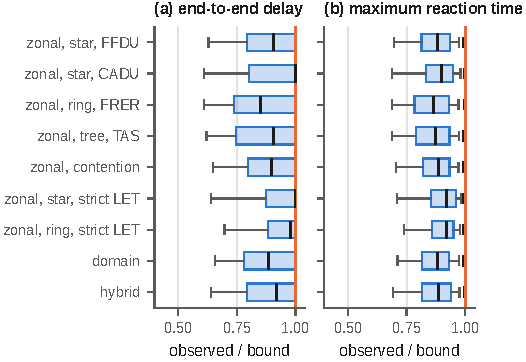
\includegraphics[width=\columnwidth]{figures/syssim}
\caption{Full-system simulation: observed delay over its bound for every
task-chain (9000 task-chains, 5 applications of 200 per setting, 4
scenarios each). Box: quartiles and median; whiskers: 5th and 95th
percentiles; tick: largest.}
\label{fig:syssim}
\end{figure}

\subsection{RQ1: number of cores and optimality gap}
\label{sec:rq1}

\paragraph{Cores and the lower bound.} \Cref{fig:sweep}(a) shows the cores
used as the sub-chain limit $\sigma$ varies, with the lower bound of
\cref{prop:lb}. \BFDU\ and \FFDU\ use 14.45 and 14.40 cores at the default point, 1.21
times the lower bound of 11.95 (1.15 to 1.36 over the instances).
Consolidation empties 1.4 cores on average. \WFDU\ spreads the load over
all 28 initial cores by construction, so its $M$ measures the spreading,
not a need. $\sigma$ barely changes the number of cores. Most task-chains
use less than 8\,\% of a core, so the cuts are mostly forced by bindings:
the fragmentation rate falls from 49\,\% at $\sigma=0.02$ to 24\,\% at
$\sigma\ge0.2$. Small sub-chains only add communications, as
\cref{fig:sweep}(b,c) shows.

\begin{figure*}[t]
\centering
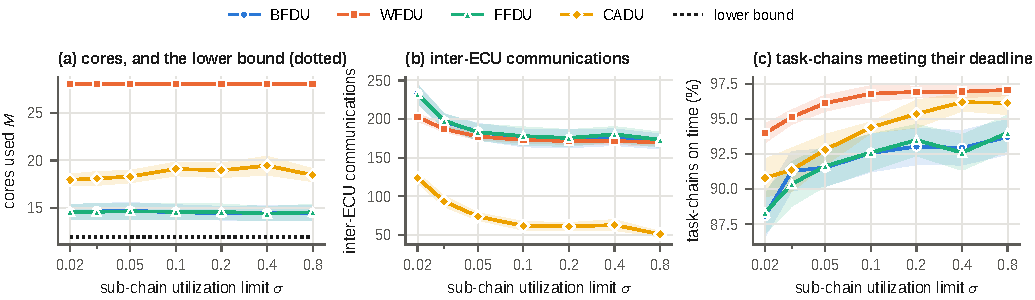
\includegraphics[width=\textwidth]{figures/sweep}
\caption{Sub-chain limit $\sigma$ and allocation rule (300 task-chains, 20
instances, 95\,\% confidence bands). \BFDU\ and \FFDU\ coincide in cores. (a) Cores
used, with the lower bound of \cref{prop:lb} (dotted). (b) Inter-ECU
communications. (c) Task-chains that meet their deadline.}
\label{fig:sweep}
\end{figure*}

\paragraph{Optimality gap.} The lower bound ignores the LET load, the
schedulability gaps and the integrality of each zone, so the ratio above
overstates the gap. The exact formulation of \cref{sec:exact} measures it.
It was run on 150 instances: 20 to 300 task-chains, 10 instances per
size, on three platforms (default; zone cores at 25\,\% speed; and 20\,\%
of replicated task-chains, 10\,\% of zone-only task-chains and 8\,MB of
memory per zone controller). On the constrained platform, no instance of
300 task-chains has an admissible mapping: the pinned tasks of some zone
alone exceed its memory, which both methods detect. Of the 140 other
instances, 134 were solved to proven optimality within 60\,s (5.3\,s on
average) and 6 stopped at the limit with their best solution, against
which the gap is then measured; the tool accepted every exact allocation.
The optimum is that of the sub-chains of step 1, without contention, over
the candidate cores of \cref{sec:exact}. \CADU\ maps only 2 of the 10
constrained instances of 200 task-chains, which \BFDU, \FFDU\ and the
exact solver all map: it fills the 8\,MB of zone memory with free
sub-chains, after which a replica finds every ECU with memory left
already running another replica of its task-chain. \Cref{fig:exact}
and \cref{tab:exact} give the result. With consolidation, \BFDU\ and
\FFDU\ are 2.3\,\% above the best allocation found on average, and equal
to it in 83\,\% of the instances. Counting only proven optima, \BFDU\ is
optimal in 113 of the 140 instances (81\,\%), and, measured against the
lower bound of the solver on the 6 unproven instances, its mean gap is at
most 2.9\,\% (2.85\,\% for \FFDU). Without consolidation they were 20\,\% above it, one to
three cores on instances that need five to twenty. The loss comes from
the order of the packing: a core opened early for a large sub-chain stays
lightly loaded, while the smaller sub-chains allocated later fill the
gaps that the pinned work leaves elsewhere; emptying such cores is what
step 3 does. \CADU\ is further from the optimum (22\,\%), on purpose: it
gives up cores to keep computations next to their devices (RQ2).

\paragraph{Other architectures.} The same study on the domain and hybrid
platforms of \cref{tab:templates} (100 more instances, all proven optimal,
in 1.4\,s on average and 11.4\,s at worst, every exact allocation
accepted by the tool; one domain instance used every candidate core of an
ECU, and solving it again with six spare cores instead of two gave the
same optimum) gives a gap of 4.4\,\% for
\BFDU\ and 4.7\,\% for \FFDU\ on the domain platform, optimal in
68\,\% and 62\,\% of the instances, and of 1.2\,\% and 1.1\,\% on the
hybrid one, optimal in 88\,\% and 90\,\% (\cref{tab:exact}). The domain
platform is the harder case: without a central computer, the free
sub-chains have no single obvious host. This study changed the method. In
its first version, a platform without a central computer gave the free
sub-chains to any ECU, in the order of the platform, which let them fill
microcontroller cores where they cost twice the utilization: on the domain
platform, \BFDU\ was 19\,\% above the optimum
on average (36 and 37\,\% at 200 and 300 task-chains) and \FFDU\
7.2\,\%. Giving them first to the ECUs with the fastest cores
(\cref{sec:other-architectures}) brought the averages down to 4.4 and
4.7\,\%. The zonal and hybrid platforms, which have a central computer,
are not affected.

\begin{figure*}[t]
\centering
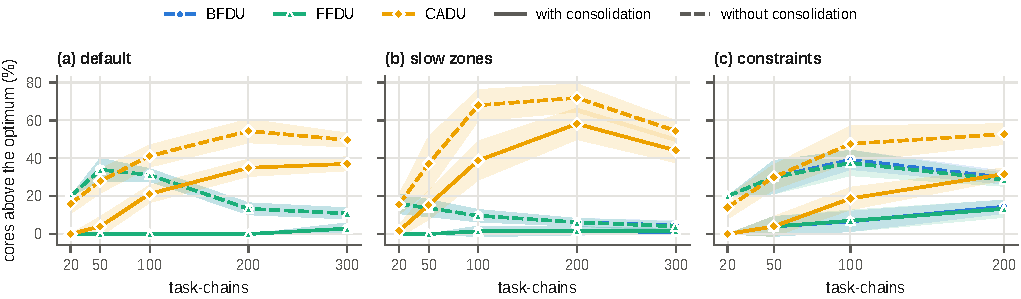
\includegraphics[width=\textwidth]{figures/exact}
\caption{Cores above the optimum found by the exact formulation (10
instances per size, 95\,\% confidence bands), with (solid) and without
(dashed) consolidation. (a) Default platform. (b) Zone cores at 25\,\%
speed. (c) Replicas, zone-only task-chains and 8\,MB of zone memory.}
\label{fig:exact}
\end{figure*}

\begin{table}[t]
\centering\footnotesize
\caption{Exact formulation against the heuristics (10 instances per row;
instances without an admissible mapping left out). Zonal platform:
default, slow zone controllers, spatial constraints; then the domain and
hybrid platforms of \cref{tab:templates}. \emph{proven}: solved to
optimality within 60\,s; \emph{opt.}: mean optimum (best found if not
proven); gaps in \% of the optimum, with consolidation / without.}
\label{tab:exact}
\setlength{\tabcolsep}{2pt}
\rowcolors{2}{brandlight}{white}
\begin{tabular}{@{}lrrrrrrr@{}}
\toprule
\rowcolor{white}
platform & chains & proven & $M_{\mathrm{LB}}$ & opt. & \BFDU & \FFDU &
\CADU \\
\midrule
default & 20 & 10/10 & 5.0 & 5.0 & 0 / 20 & 0 / 20 & 0 / 16 \\
default & 50 & 10/10 & 5.0 & 5.0 & 0 / 34 & 0 / 34 & 4 / 28 \\
default & 100 & 10/10 & 5.0 & 6.1 & 0 / 31 & 0 / 31 & 21 / 41 \\
default & 200 & 10/10 & 7.4 & 9.1 & 0 / 13 & 0 / 13 & 35 / 54 \\
default & 300 & 10/10 & 11.6 & 13.7 & 3 / 11 & 3 / 11 & 37 / 50 \\
slow zones & 20 & 10/10 & 5.0 & 5.2 & 0 / 16 & 0 / 16 & 2 / 16 \\
slow zones & 50 & 10/10 & 5.0 & 6.0 & 0 / 14 & 0 / 14 & 15 / 37 \\
slow zones & 100 & 9/10 & 5.4 & 8.2 & 1 / 10 & 1 / 10 & 39 / 68 \\
slow zones & 200 & 10/10 & 10.0 & 13.1 & 2 / 6 & 2 / 6 & 58 / 72 \\
slow zones & 300 & 7/10 & 15.7 & 19.5 & 1 / 5 & 1 / 4 & 44 / 54 \\
constraints & 20 & 10/10 & 5.0 & 5.0 & 0 / 20 & 0 / 20 & 0 / 14 \\
constraints & 50 & 10/10 & 5.0 & 5.0 & 4 / 30 & 4 / 30 & 4 / 30 \\
constraints & 100 & 8/10 & 5.0 & 5.9 & 7 / 39 & 7 / 38 & 19 / 48 \\
constraints & 200 & 10/10 & 7.6 & 9.1 & 14 / 30 & 13 / 29 & 32 / 53 \\
\midrule
domain & 20 & 10/10 & 5.0 & 5.0 & 0 / 14 & 0 / 0 & 0 / 4 \\
domain & 50 & 10/10 & 5.0 & 5.0 & 0 / 50 & 0 / 18 & 6 / 24 \\
domain & 100 & 10/10 & 5.0 & 5.1 & 10 / 83 & 2 / 37 & 38 / 63 \\
domain & 200 & 10/10 & 7.0 & 8.1 & 7 / 50 & 11 / 26 & 36 / 71 \\
domain & 300 & 10/10 & 10.8 & 12.4 & 5 / 34 & 11 / 34 & 26 / 53 \\
hybrid & 20 & 10/10 & 5.0 & 5.0 & 0 / 20 & 0 / 20 & 0 / 16 \\
hybrid & 50 & 10/10 & 5.0 & 5.0 & 0 / 34 & 0 / 34 & 2 / 24 \\
hybrid & 100 & 10/10 & 5.0 & 5.7 & 2 / 41 & 2 / 41 & 14 / 44 \\
hybrid & 200 & 10/10 & 7.2 & 8.7 & 1 / 19 & 1 / 19 & 30 / 49 \\
hybrid & 300 & 10/10 & 11.2 & 13.0 & 3 / 15 & 2 / 14 & 33 / 48 \\
\bottomrule
\end{tabular}
\end{table}


\paragraph{Against metaheuristics.} Simulated annealing (SA) and a
genetic algorithm (GA) solve the same problem: the same sub-chains, every
constraint and the schedulability test, with the number of cores as the
objective (\cref{app:baselines}). \Cref{fig:baselines} plots the gap to
the proven optimum against the time, on the ten default instances of each
size. The packing rules are optimal on all of them up to 200 task-chains
and 2.9\,\% above at 300, in 2 to 32\,ms. SA needs $10^6$ moves, 3.7 to
13.0\,s, to come as close (2.0, 0, 0 and 0.8\,\%); with $2\cdot10^5$
moves it stays 2.2 to 6.7\,\% above. The GA degrades with the size: 0,
3.3, 6.6 and 17.9\,\% after 100 generations, which take up to 61\,s.
On these instances the exact solver (0.27 to 6.3\,s on average on the
default platform) is faster than both metaheuristics and proves
optimality. Both metaheuristics minimize the cores only, so they are
given the deadline local search of the heuristic on their best mapping.
They then keep as many task-chains on time as the packing rules at 50
task-chains (97\,\%), and 2.6 to 6.4 points fewer beyond (88 to 89\,\% at
300, against 94\,\%).

\paragraph{The harder platforms.} The default platform is where the
packing rules are best, so \cref{tab:baselines-platforms} repeats the
comparison on the three platforms where they are furthest from the
optimum. With slow zones, the packing rules stay within 1.7\,\% of the
best allocation known, the GA within 0.9\,\% (in 4 to 44\,s), and SA is
no better than the rules (1.0 to 3.9\,\%). On the domain platform, the
packing rules are up to 11.1\,\% above (\FFDU; \BFDU\ up to 9.7\,\%),
and the GA closes most of that gap (0 to 4.0\,\%, in 7 to 77\,s), while
SA does not (up to 20\,\%). On the constrained
platform, no method is close at 200 task-chains: the packing rules are
13 to 14\,\% above the optimum, the GA 21\,\%, and SA finds no admissible
mapping on half of the instances. The exact solver handles all these
instances in 0.1 to 30\,s on average, proves 104 of the 110 optima, and
finds an allocation at least as good as every other method on every
instance. A metaheuristic therefore adds nothing on the default
platform; where the packing rules fall short, a GA run for tens of
seconds recovers most of the gap on two of the three platforms, and the
exact formulation all of it, in a comparable time. The packing rules
are the tool for exploring a design space, and the exact formulation, or
a GA beyond its reach, the tool for the final sizing.

\begin{table}[t]
\centering\footnotesize
\caption{The heuristic against the metaheuristics on the hard platforms
of \cref{tab:exact} (10 instances per size; on the constrained platform,
no instance of 300 task-chains is feasible). Gap: cores above the best
allocation known (the exact solver or any method), \%, mean; on time:
task-chains that meet their deadline, \%, with the deadline local search
applied to every method; SA: $10^6$ moves, GA: 100 generations, with
their CPU times; --: no admissible mapping found on some instances (SA on
5 of the 10 constrained instances of 200 task-chains).}
\label{tab:baselines-platforms}
\setlength{\tabcolsep}{2.4pt}
\begin{tabular}{@{}lrrrrrrrrr@{}}
\toprule
 & & \multicolumn{4}{c}{gap (\%)} & \multicolumn{2}{c}{on time (\%)} & \multicolumn{2}{c@{}}{time (s)} \\
\cmidrule(lr){3-6}\cmidrule(lr){7-8}\cmidrule(l){9-10}
chains & inst. & \BFDU & \FFDU & SA & GA & \FFDU & SA & SA & GA \\
\midrule
\rowcolor{white}\multicolumn{10}{@{}l}{\emph{slow zones}} \\
\quad 50 & 10 & 0.0 & 0.0 & 3.7 & 0.0 & 96.6 & 97.0 & 2.9 & 4.4 \\
\quad 100 & 10 & 1.4 & 1.4 & 3.9 & 0.0 & 94.4 & 92.9 & 5.0 & 12 \\
\quad 200 & 10 & 1.7 & 1.7 & 3.7 & 0.8 & 93.5 & 87.8 & 7.9 & 28 \\
\quad 300 & 10 & 1.0 & 1.5 & 1.0 & 0.9 & 92.4 & 86.3 & 9.0 & 44 \\
\rowcolor{white}\multicolumn{10}{@{}l}{\emph{constraints}} \\
\quad 50 & 10 & 4.0 & 4.0 & 0.0 & 0.0 & 96.6 & 96.4 & 2.9 & 4.8 \\
\quad 100 & 10 & 6.7 & 7.0 & 7.3 & 5.7 & 97.8 & 94.6 & 5.9 & 14 \\
\quad 200 & 10 & 14.4 & 13.3 & -- & 21.4 & 93.9 & -- & 3.8 & 21 \\
\rowcolor{white}\multicolumn{10}{@{}l}{\emph{domain}} \\
\quad 50 & 10 & 0.0 & 0.0 & 0.0 & 0.0 & 98.8 & 98.8 & 4.4 & 6.6 \\
\quad 100 & 10 & 9.7 & 2.0 & 20.0 & 4.0 & 96.0 & 97.7 & 8.6 & 19 \\
\quad 200 & 10 & 7.4 & 11.1 & 8.9 & 0.0 & 96.2 & 96.3 & 16 & 46 \\
\quad 300 & 10 & 4.9 & 10.6 & 8.2 & 2.6 & 94.4 & 92.3 & 20 & 77 \\
\bottomrule
\end{tabular}
\end{table}


\begin{figure*}[t]
\centering
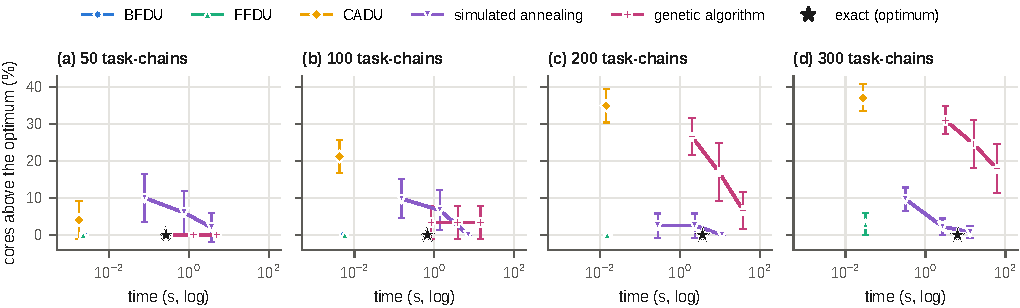
\includegraphics[width=\textwidth]{figures/baselines}
\caption{Cores above the optimum against the time to map, default
platform (10 instances per size, 95\,\% confidence intervals). The
heuristic rules with consolidation (\BFDU\ and \FFDU\ coincide),
simulated annealing with $2\cdot10^4$, $2\cdot10^5$ and $10^6$ moves,
the genetic algorithm with 5, 25 and 100 generations (CPU time), and the
exact formulation (wall time, two threads).}
\label{fig:baselines}
\end{figure*}

\begin{table}[t]
\centering\footnotesize
\caption{Time to map one application. Exact: wall time of the constraint
program (two threads, 60\,s limit), mean and worst over the three
zonal platforms of \cref{tab:exact}, and the instances proven optimal. The
others: mean CPU time on the default platform (10 instances), the
heuristic with consolidation, the simulated annealing with $10^6$ moves and
the genetic algorithm with 100 generations.}
\label{tab:speed}
\setlength{\tabcolsep}{3pt}
\rowcolors{2}{brandlight}{white}
\begin{tabular}{@{}rrrrrrrr@{}}
\toprule
\rowcolor{white}
 & \multicolumn{3}{c}{exact (s)} & \multicolumn{2}{c}{heuristic (ms)} &
 \multicolumn{2}{c@{}}{baselines (s)} \\
\cmidrule(lr){2-4}\cmidrule(lr){5-6}\cmidrule(l){7-8}
\rowcolor{white}
chains & mean & worst & proven & \FFDU & \CADU & SA & GA \\
\midrule
50 & 0.37 & 1.8 & 30/30 & 2 & 2 & 3.7 & 5.0 \\
100 & 7.83 & 60.2 & 27/30 & 6 & 4 & 7.1 & 14.2 \\
200 & 4.45 & 13.1 & 30/30 & 15 & 14 & 11.2 & 37.9 \\
300 & 17.93 & 60.9 & 17/20 & 32 & 27 & 13.0 & 61.4 \\
\bottomrule
\end{tabular}
\end{table}


\Cref{fig:architecture-results} varies the speed of the zone cores. At a
quarter of the speed of the central computer, the pinned work of the zones
needs 12.8 zone cores (\BFDU), and the task-chains lose a point of deadline
satisfaction because every response time in a zone grows. From 75\,\%
speed upwards the zones need 6 cores or fewer, and the central computer is
the bottleneck. A cheap microcontroller-class zone controller thus costs
cores in proportion to its pinned work, not to the whole application.

\begin{figure}[t]
\centering
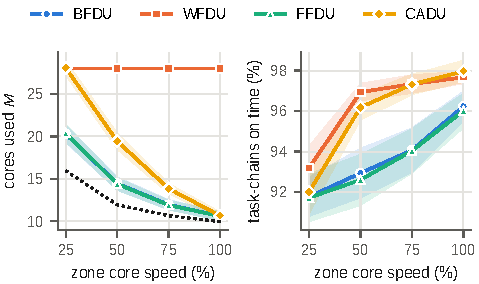
\includegraphics[width=\columnwidth]{figures/architecture}
\caption{Speed of the zone cores (central computer at 100\,\%). Left:
cores used and lower bound (dotted). Right: task-chains that meet their
deadline.}
\label{fig:architecture-results}
\end{figure}

\subsection{RQ2: communication awareness}
\label{sec:rq2}

\CADU\ keeps a computation next to the device it serves whenever the zone
has room. At the default point it removes 64\,\% of the inter-ECU
communications (63 instead of 177; paired difference $-114\pm15$). The
largest network bound falls from \SI{1.40}{ms} to \SI{0.58}{ms}, and the
share of task-chains that meet their deadline rises from 92.9 to 96.2\,\%
(paired difference $+3.3\pm1.2$ points). The price is $+5.0\pm0.4$ cores:
the work kept in the zones runs on cores at half speed, so the application
load grows from 10.2 to 13.7 cores. \Cref{fig:tradeoff} shows the
trade-off for every instance. \BFDU\ and \FFDU\ are the cheapest. \CADU\
dominates \WFDU\ in cores, at almost the same deadline satisfaction.
\WFDU's good timing comes from spreading: every core is lightly loaded and
response times are short. Affinity (trying the cores of the same
task-chain first) removes all communications between cores of one ECU for
\WFDU, but changes the bin-packing rules by less than 0.5 point, because
those rules already pack the sub-chains of a task-chain together.

\begin{figure}[t]
\centering
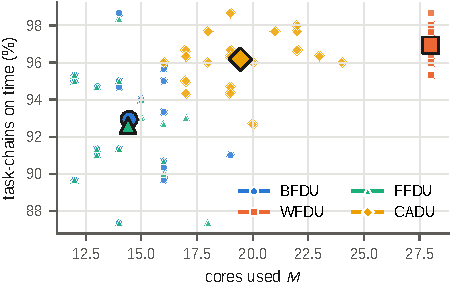
\includegraphics[width=\columnwidth]{figures/tradeoff}
\caption{Cores against task-chains that meet their deadline, every
instance of the default point (small markers) and means (large markers):
\CADU\ trades cores for deadline satisfaction.}
\label{fig:tradeoff}
\end{figure}

\subsection{RQ3: network design and communication}
\label{sec:rq3}

\paragraph{Rate, preemption, message sizes.} \Cref{fig:network}(a,b)
varies the link rate, frame preemption and the message sizes. At
100\,Mbit/s, the port of the central computer carries all the traffic
between zones in a bin-packed mapping: its load reaches 57\,\%, and only
75\,\% of the task-chains meet their deadline, against 95\,\% with \CADU,
whose port load is three times lower. With a third of the messages large
(up to 64\,kB, a sensor-heavy application), even 1\,Gbit/s overloads that
port with bin packing (69\,\% load, close to the 75\,\% idle slope, and
some ports above it): 73\,\% of the task-chains meet their deadline,
against 95\,\% with \CADU. Frame preemption changes almost nothing,
because the blocking of one best-effort frame (\SI{12}{\micro s} at
1\,Gbit/s) is small next to the LET sampling delays of milliseconds.

\begin{figure*}[t]
\centering
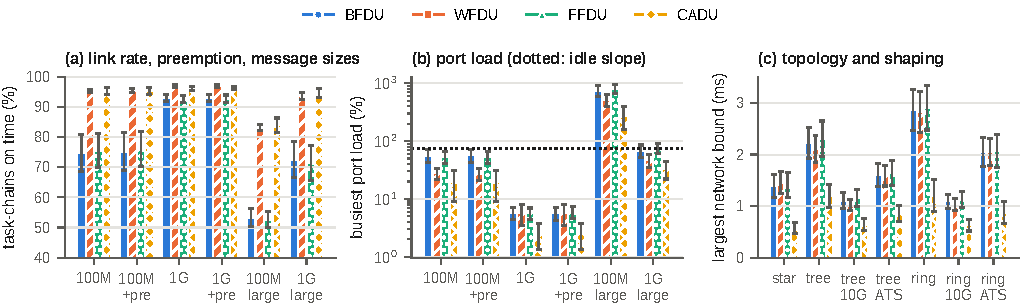
\includegraphics[width=\textwidth]{figures/network}
\caption{Network design. (a) Task-chains that meet their deadline and (b)
busiest port load (log scale; above the idle slope, flows have no bound),
for link rates of 100\,Mbit/s and 1\,Gbit/s, with frame preemption (+pre)
and with large sensor messages. (c) Largest network bound for the three
topologies, with a 1 or 10\,Gbit/s backbone, and with ATS instead of CBS.}
\label{fig:network}
\end{figure*}

\paragraph{Topology and shaping.} \Cref{fig:network}(c) compares
topologies at the default load. A tree or a ring adds switch ports to the
routes, which raises the largest bound from \SI{1.4}{ms} (star) to
\SI{2.2}{ms} (tree) and \SI{2.9}{ms} (ring) with \BFDU. On the ring, the
cyclic dependencies make the bursts grow around the ring. ATS cuts this
growth: the regulators reset the bursts at every switch, and the largest
bound falls to \SI{1.6}{ms} on the tree and \SI{2.0}{ms} on the ring, with
the same 1\,Gbit/s links. A 10\,Gbit/s backbone brings both topologies
near \SI{1.1}{ms}. Deadline satisfaction moves by less than one point: at
this load, LET sampling, not the network, dominates the reaction times.

\paragraph{Frame replication.} \Cref{fig:frer-results} adds FRER on the ring for
10 to 30\,\% of replicated task-chains. Replication sends a second member
stream around the other side of the ring, so the busiest backbone link
carries up to 1.4 points more load, and the largest bound grows by about
2\,ms with CBS (from 2.1 to 4.1\,ms at 30\,\%) and by 1.4\,ms with ATS (from
1.5 to 2.9\,ms). The bound of a replicated flow is that of its longer
route, and the burst after the elimination grows with the difference
between the two routes (\cref{prop:frer}). Deadline satisfaction drops by
at most 0.4 point. Making the redundancy of the replicated task-chains
survive a link or switch failure therefore costs little at this load, and
less with ATS than with CBS, since the member streams do not accumulate
bursts around the ring.

\begin{figure}[t]
\centering
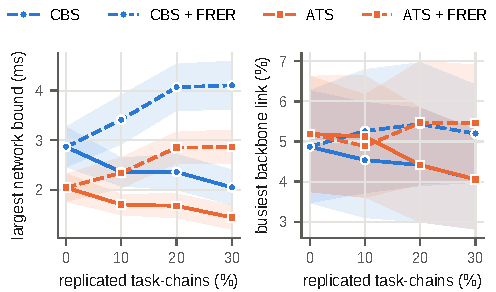
\includegraphics[width=\columnwidth]{figures/frer}
\caption{Frame replication on the ring (\BFDU): largest network bound and
busiest backbone link, with CBS or ATS, against the share of replicated
task-chains.}
\label{fig:frer-results}
\end{figure}

\paragraph{Implicit communication or strict LET.} \Cref{tab:communication}
maps the same applications with the two schemes of
\cref{sec:execution}. The cores do not change, and the allocation barely
does: only the local search, which sees other deadlines, moves a few
sub-chains. Strict LET removes the response time from the release
jitter of every flow ($J_h=C^{\LET}$ instead of $R_{\mathrm{prod}}+
T^{\LET}$), so the largest network bound falls by 19\,\% with \FFDU\ (by
270\,\si{\micro s} $\pm$ 80) and by 15\,\% on the ring. But every
crossing between cores now waits for the end of the period of its
producer, so the mean reaction bound grows by 39\,ms with \FFDU\ (by 19\,\%)
and by 16\,ms with \CADU, and the task-chains on time drop by 30 points
with \FFDU\ and 16 with \CADU\ ($\pm$ 2.2 and 1.4). The cause is
structural: a single-pattern task-chain of period $T$ with $c$ crossings
has a reaction bound of at least $(c+1)T$ with implicit communication
and $(2c+1)T$ with strict LET, so a deadline of $3T$ admits one crossing
with the first and none with the second. With deadlines at 500\,\% the gap
narrows to 4.2 and 1.5 points. The determinism of strict LET is therefore
paid in deadlines, and the fewer crossings of \CADU\ halve the bill:
strict LET needs a communication-aware allocation, or deadlines set for
it.

\begin{table}[t]
\centering\footnotesize
\caption{Implicit communication or strict LET between cores (300
task-chains, 20 instances). on time: task-chains that meet their deadline
(\%); $\bar\Delta$: mean bound of the maximum reaction time (ms); $d$:
largest network bound (\si{\micro s}).}
\label{tab:communication}
\setlength{\tabcolsep}{2.6pt}
\begin{tabular}{@{}lrrrrrr@{}}
\toprule
 & \multicolumn{3}{c}{\FFDU} & \multicolumn{3}{c@{}}{\CADU} \\
\cmidrule(lr){2-4}\cmidrule(l){5-7}
 & on time & $\bar\Delta$ & $d$ & on time & $\bar\Delta$ & $d$ \\
\midrule
\rowcolor{white}\multicolumn{7}{@{}l}{\emph{default point}} \\
\quad implicit & 92.6 & 205.6 & 1415 & 96.2 & 191.2 & 578 \\
\quad strict LET & 62.4 & 244.6 & 1145 & 79.7 & 207.0 & 402 \\
\rowcolor{white}\multicolumn{7}{@{}l}{\emph{deadlines at 500\,\%}} \\
\quad implicit & 99.5 & 208.9 & 1496 & 99.6 & 195.6 & 573 \\
\quad strict LET & 95.3 & 246.6 & 1109 & 98.1 & 222.4 & 435 \\
\rowcolor{white}\multicolumn{7}{@{}l}{\emph{ring, three classes}} \\
\quad implicit & 91.3 & 208.7 & 37135 & 96.0 & 191.7 & 40615 \\
\quad strict LET & 61.7 & 248.5 & 31650 & 79.3 & 207.5 & 35916 \\
\bottomrule
\end{tabular}
\end{table}


\paragraph{The whole vehicle.} On the whole vehicle (\cref{tab:vehicle},
2000 task-chains), the network matters more. Raising the backbone and the
link of the central computer to 10\,Gbit/s increases the task-chains that
meet their deadline from 81.4 to 88.3\,\% (\BFDU). Splitting the LET
traffic into classes by period does not help with CBS. With two classes,
the low class (periods above 20\,ms) gets bounds of up to \SI{99}{ms}, and
deadline satisfaction falls to 83\,\%. Three classes with proportional idle
slopes (\cref{eq:slopes}) recover 88.8\,\%, close to one class. TAS with
one window is close to CBS (88.0\,\%); with three windows it loses four
points, because each class only gets its own window. ATS gives the lowest
bounds with one class (\SI{2.8}{ms}, against \SI{3.9}{ms} for CBS) and
also with three (\SI{3.1}{ms}, against \SI{36}{ms}), and the best deadline
satisfaction (89.0\,\% with three classes).

\subsection{RQ4: spatial constraints, core types and contention}
\label{sec:rq4}

\paragraph{Spatial constraints.} \Cref{fig:constraints}(a) adds constraints
one at a time. Replicating 10 to 30\,\% of the task-chains with ECU
separation costs at most 0.5 core (\BFDU). The replicas replace other
task-chains, so that the application keeps its number of task-chains, and
only task-chains that are not heavy are replicated; the applications with
replicas are therefore slightly lighter than those without, and this
figure compares the two only roughly. Two replicas may not share the
central computer, so one of each pair runs in a zone (central cores fall
from 6.7 to 4.7, zone cores rise from 7.8 to 10.2), mostly on zone cores
that were already there. Separating replicas by core only needs 13.7 cores instead
of 14.6, but it puts both replicas on the central computer, where one
failure of that ECU loses both. Forbidding
the central computer to 20\,\% of the task-chains (zone-only safety
functions) costs 1.2 cores. Co-location of 30\,\% of consecutive free tasks
costs nothing measurable. A memory of 8\,MB per zone controller makes 55\,\%
of the applications infeasible. In all of them, the pinned tasks of some
zone alone exceed 8\,MB, which no mapping can fix; by
\cref{prop:memory}, and because a free sub-chain can always go to a new
core of the central computer here, this is the only possible cause.

\begin{figure*}[t]
\centering
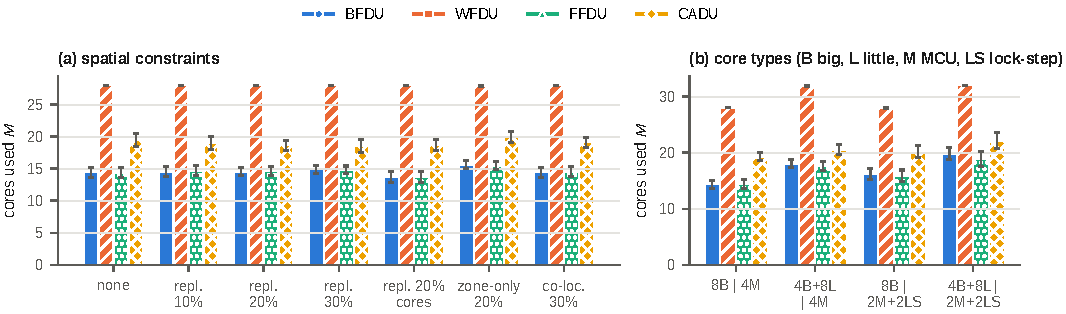
\includegraphics[width=\textwidth]{figures/constraints}
\caption{Cores used under (a) spatial constraints and (b) heterogeneous
core types, with every WCET within $\pm30\,\%$ of its speed ratio on each
type (B: big, L: little, M: MCU, LS: lock-step; 10\,\% of the task-chains
on lock-step cores when LS cores exist).}
\label{fig:constraints}
\end{figure*}

\paragraph{Core types.} \Cref{fig:constraints}(b) varies the core types,
with per-type WCET factors drawn within $\pm30\,\%$ of the speed ratio.
Replacing half of the big cores of the central computer by twice as many
little ones (40\,\% speed) adds 3.7 cores for \BFDU. Replacing half of
the zone cores by lock-step cores, for the 10\,\% of safety task-chains
that need them, adds 1.8 cores; both
together add 5.5 cores (19.8 instead of 14.4). Splitting the zone cores
between safety and other work removes packing flexibility in every zone.
This cost of dedicated safety hardware is visible only with a type-aware
model.

\paragraph{Memory contention.} \Cref{fig:contention} sets the latency of a
memory request from 0 to 100\,ns, with 1000 requests per millisecond of
WCET. At 100\,ns a request may wait \SI{0.3}{\micro s} on a zone
controller of four cores and \SI{0.7}{\micro s} on the central computer of
eight (more when cores are added there), a contention of 30 to 70\,\% of the reference WCET. The application
load grows from 10.2 to 15.0 cores, and \BFDU\ needs 22.2 cores instead of
14.4 (+54\,\%). \CADU\ suffers less (+22\,\%, from 19.5 to 23.7 cores),
because its zone cores run at half speed, so the same wait is a smaller
share of their WCETs, and its central computer uses few cores. The gap
between packing and communication awareness thus shrinks from five cores
to 1.5. Ignoring contention, as WCET-inclusive models do, would hide that
the number of cores a heavily loaded central computer needs grows with
the cores themselves.

\begin{figure}[t]
\centering
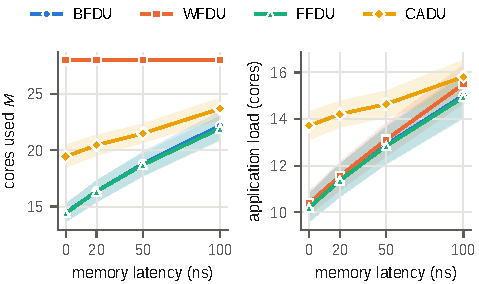
\includegraphics[width=\columnwidth]{figures/contention}
\caption{Shared-memory contention: cores used and application load
against the latency of a memory request (1000 requests per ms of WCET,
round robin).}
\label{fig:contention}
\end{figure}

\subsection{RQ5: deadline local search and margins}
\label{sec:rq5}

\paragraph{Local search.} \Cref{fig:deadlines} varies the deadline from 200
to 600\,\% of the sum of the pattern periods. At the default 300\,\%,
without the local search, the bin-packing rules leave 88.8\,\% of the
task-chains on time; the local search raises this to 92.9\,\% with 12 kept
moves, in \SI{6}{ms} of CPU time per design point. It is most effective
where cores have room: it lifts \WFDU\ from 79 to 97\,\% at 300\,\% and
from 49 to 87\,\% at 200\,\%, while \BFDU\ only goes from 55 to 60\,\% at
200\,\%: tightly packed cores leave little room for the moves. No move can
remove a communication between two pinned sub-chains in different zones, so
a task-chain whose deadline is shorter than the sampling delays of such
communications stays late (\cref{sec:example}).

\begin{figure}[t]
\centering
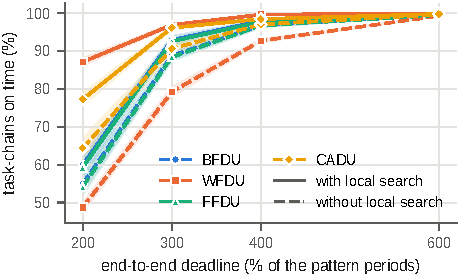
\includegraphics[width=\columnwidth]{figures/deadlines}
\caption{End-to-end deadline, with (solid) and without (dashed) the
deadline-driven local search.}
\label{fig:deadlines}
\end{figure}

\paragraph{LET cost and utilization cap.} The LET cost scales with
$c_{\LET}$. At \SI{200}{\micro s} the LET tasks load 4.6 cores, and \BFDU\
needs 18.9 cores instead of 14.4. The utilization cap sets the margin:
from $\varphi=1$ to $0.6$, the critical scaling factor grows from 1.00 to
1.67, while the cores grow from 11.5 to 21.2 (\BFDU). At $\varphi=1$,
0.7\,\% of the cores are unschedulable after priority assignment, and the
relocation moves repair all of them.

\paragraph{Margins.} \Cref{fig:margins} compares two ways to obtain a
margin on the real WCETs. A WCET margin of $m$\,\% inflates every WCET and
gives the factor $\lambda(1+m/100)$ on the real WCETs. Sizing for
$\lambda^\star$ (\cref{sec:sizing}) lowers $\varphi$ instead. For the same
guaranteed factor, both need about the same number of cores: 18.3 cores for
a 20\,\% margin (factor 1.49) and 18.5 for $\lambda^\star=1.5$ (\BFDU).
Sizing, however, guarantees the target directly and reports it, runs at
most nine design points, and keeps the real WCETs for every other metric.

\begin{figure}[t]
\centering
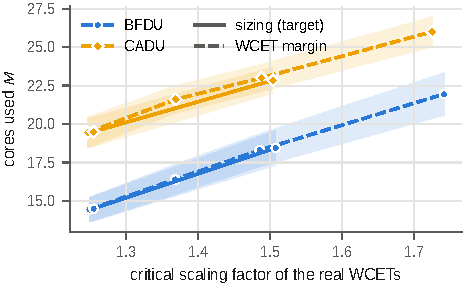
\includegraphics[width=\columnwidth]{figures/margins}
\caption{Cores against the critical scaling factor guaranteed on the real
WCETs: WCET margins of 0, 10, 20, 40\,\% (dashed) and sizing for targets
1.1, 1.25, 1.5 (solid).}
\label{fig:margins}
\end{figure}

\subsection{RQ6: the life of a platform}
\label{sec:rq6}

\Cref{fig:lifecycle} sizes the platform at the SOP for 300 task-chains with
a provisioning cap $\varphi_{\mathrm{SOP}}$ from 0.5 to 0.8, then adds ten
software updates of 15 task-chains each (+50\,\% of software in all) up to
the design cap of 0.8. A platform sized at the design cap absorbs no update
with \BFDU: its cores are full, and the new pinned drivers need room in
their zones. Every step of provisioning buys updates: 1.3 updates at
$\varphi_{\mathrm{SOP}}=0.7$ for 2.8 more cores, 3.8 at 0.6 for 6.8 more,
and 6.5 at 0.5 for 12.1 more (26.6 cores). The relation is close to linear
in the cores, about one update for two cores here. \WFDU\ is a special
case: in these experiments it uses all 28 initial cores (29 at
$\varphi_{\mathrm{SOP}}=0.5$), and so absorbs
about five updates whatever the cap, but at a cost close to that of the
most provisioned \BFDU\ platform. \CADU\ absorbs updates at the price of
its extra cores, with the best deadline satisfaction along the life (96\,\%
against 91--93\,\%). The critical scaling factor of a \BFDU\ platform
falls to 1.26--1.39 after the first update and to about 1.26 after the
second, whatever its provisioning (\cref{fig:lifecycle}(b)):
an update fills some core up to the design cap, and the factor of the
platform is that of its fullest core. Provisioning therefore buys
updates, not margin.

\begin{figure}[t]
\centering
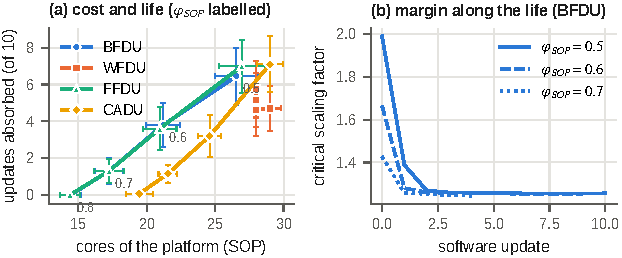
\includegraphics[width=\columnwidth]{figures/lifecycle}
\caption{Life of a platform: (a) cores bought at the SOP against the
software updates absorbed (of ten updates of 15 task-chains), for
$\varphi_{\mathrm{SOP}}$ from 0.5 to 0.8; (b) critical scaling factor
after each update (\BFDU), averaged over the platforms that have absorbed
every update so far.}
\label{fig:lifecycle}
\end{figure}

\subsection{RQ7: other E/E architectures}
\label{sec:rq7}

\Cref{fig:dse} maps the same applications (the same generator seeds) of
100 to 300 task-chains onto the four platforms of \cref{tab:templates}.
The sensors and actuators are wired to the ECUs that are not central
computers, so the bindings follow each architecture: five zone
controllers in the zonal platform, five domain controllers in the domain
one, the ADAS controller and the four zones in the hybrid one, all twelve
ECUs in the distributed one.

\paragraph{Cores.} At 300 task-chains the hybrid platform needs the
fewest cores with \FFDU\ (13.2, lower bound 11.4), then the domain one
(13.35, 11.1) and the zonal one (14.4, 11.95); the ratio to the lower
bound is 1.16, 1.20 and 1.21. Both alternatives save about a core over
the zonal platform for the same reason: part of the pinned work runs on
ECUs with big cores, a fifth of it on the ADAS controller of the hybrid
platform and two fifths on the ADAS and infotainment controllers of the
domain one, instead of on microcontroller cores at half speed, which
lowers the bound itself. The distributed platform runs out of room. It needs at least one
core per ECU (12), and with at most two cores per small ECU and four on
the ADAS controller, \FFDU\ maps 95\,\% of the applications of 200
task-chains and 50\,\% of those of 300 (\CADU: 100 and 75\,\%). The
failures are sub-chains that find every allowed ECU at its largest number
of cores; placing the bound sub-chains before the free ones, so that
these cannot take the cores of the ADAS controller, maps fewer
applications, not more. Its 100\,Mbit/s network is the most loaded
(23\,\% on the busiest port at 300 task-chains with \FFDU, against at
most 6\,\% elsewhere).

\paragraph{Communications and timing.} At 300 task-chains, \FFDU\ creates
166 to 180 inter-ECU communications on the three platforms that map every
application, and \CADU\ 62 to 74: a reduction of 65\,\% on the zonal
and hybrid platforms and of 56\,\% on the domain one. The
share of task-chains on time is within one point between them (92.6 to
93.1\,\% with \FFDU, 96.2 to 96.7\,\% with \CADU). The zonal platform is
therefore not the cheapest in cores for this software: what matters most
is the speed of the cores that run the pinned work.

\begin{figure*}[t]
\centering
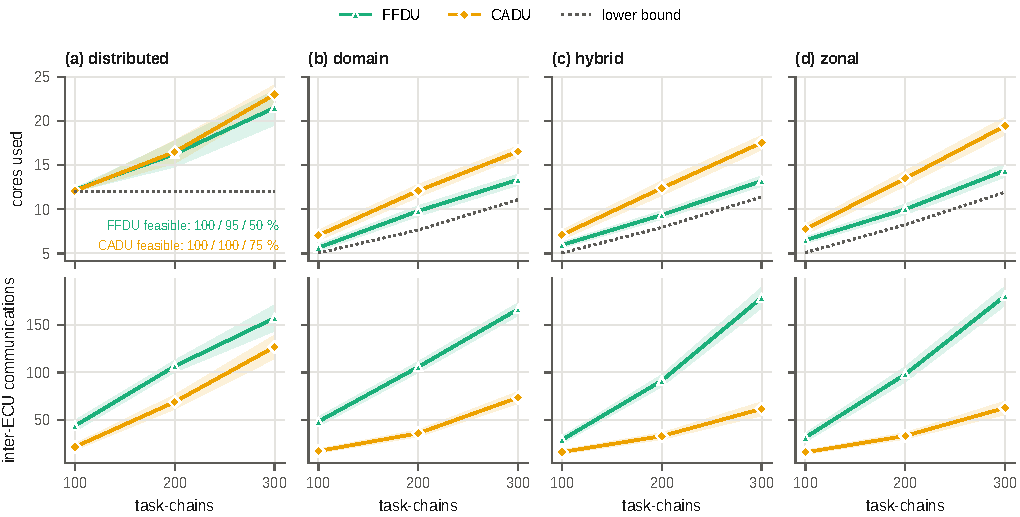
\includegraphics[width=\textwidth]{figures/dse}
\caption{The same applications on four E/E architectures
(\cref{tab:templates}; 20 instances, 95\,\% confidence bands, means over
the feasible instances). Top: cores used and lower bound (dotted).
Bottom: inter-ECU communications. Only the distributed platform has
instances without an admissible mapping; their share is given in (a), and
its means are over fewer, different instances for each rule and size.}
\label{fig:dse}
\end{figure*}

\subsection{RQ8: ablation and the rules of practice}
\label{sec:rq8}

\paragraph{Ablation.} \Cref{tab:ablation} removes one part of the method
at a time, on the default point and on a stressed one ($\varphi=1$, so
that some cores are unschedulable after step 4, and deadlines at
200\,\%). Consolidation saves $1.40\pm0.28$ cores with \FFDU\ and
$1.85\pm0.35$ with \CADU\ (default), and $0.90\pm0.21$ and $1.50\pm0.32$
(stressed). The cores it empties also leave less room, so without it
$3.65\pm1.19$ points more task-chains are on time with \FFDU\ (default).
The deadline-driven local search adds $4.18\pm0.96$ points of task-chains
on time with \FFDU\ and $5.50\pm1.37$ with \CADU\ (default), and
$4.60\pm1.26$ and $12.83\pm2.44$ (stressed), without changing the cores.
The relocation moves only matter when cores are unschedulable: in the
stressed setting, 0.7\,\% of the cores of \FFDU\ are unschedulable after
the priority assignment, and without relocation they stay so (the
apparent saving of $0.20\pm0.19$ cores is that of a mapping that is not
admissible). Adding the swap moves of the first version of step 5 before
the relocation moves changed no result in either setting, nor in any other
experiment (\cref{sec:placement}); they are now an option, off by
default. Affinity makes no significant difference to the packing rules
(every paired interval contains zero). Without all of them, \FFDU\ needs $1.40\pm0.28$
more cores and loses $6.58\pm1.11$ points of task-chains on time
(default), and $15.45\pm2.28$ points when stressed.

\begin{table*}[t]
\centering\footnotesize
\caption{Ablation: the method with one part removed (300 task-chains, 20
instances). Default: the default platform. Stressed: utilization cap
$\varphi=1$ and deadlines at 200\,\% of the sum of the pattern periods.
$M$: cores used; on time: task-chains that meet their deadline (\%);
sched.: cores schedulable at the end (\%, \FFDU).}
\label{tab:ablation}
\setlength{\tabcolsep}{4pt}
\rowcolors{2}{brandlight}{white}
\begin{tabular}{@{}lrrrrrrrrrr@{}}
\toprule
\rowcolor{white}
 & \multicolumn{5}{c}{default} & \multicolumn{5}{c@{}}{stressed} \\
\cmidrule(lr){2-6}\cmidrule(l){7-11}
\rowcolor{white}
 & \multicolumn{2}{c}{\FFDU} & \multicolumn{2}{c}{\CADU} & &
 \multicolumn{2}{c}{\FFDU} & \multicolumn{2}{c}{\CADU} & \\
\rowcolor{white}
variant & $M$ & on time & $M$ & on time & sched. & $M$ & on time & $M$ &
on time & sched. \\
\midrule
full method & 14.40 & 92.6 & 19.45 & 96.2 & 100.0 & 11.45 & 61.3 & 16.15 & 80.9 & 100.0 \\
no affinity & 14.40 & 92.6 & 19.40 & 96.2 & 100.0 & 11.45 & 61.2 & 16.20 & 80.7 & 100.0 \\
no consolidation & 15.80 & 96.2 & 21.30 & 97.9 & 100.0 & 12.35 & 57.1 & 17.65 & 87.0 & 100.0 \\
with swap moves & 14.40 & 92.6 & 19.45 & 96.2 & 100.0 & 11.45 & 61.3 & 16.15 & 80.9 & 100.0 \\
no relocation moves & 14.40 & 92.6 & 19.45 & 96.2 & 100.0 & 11.25 & 60.7 & 15.95 & 80.8 & 99.3 \\
no local search & 14.40 & 88.4 & 19.45 & 90.7 & 100.0 & 11.45 & 56.7 & 16.15 & 68.1 & 100.0 \\
none of them & 15.80 & 86.0 & 21.30 & 90.7 & 100.0 & 12.30 & 45.6 & 17.55 & 68.6 & 99.3 \\
\bottomrule
\end{tabular}
\end{table*}


\paragraph{Rules of practice.} \Cref{tab:practice} compares the method
with three rules a practitioner might apply. Keeping task-chains whole,
cut only where their bindings force it ($\sigma=\varphi$), costs no
significant core ($+0.15\pm0.23$), and keeps $1.40\pm1.06$ points more
task-chains on time with $7.2\pm6.1$ fewer communications on this point;
the next paragraph shows where it fails. Putting all free software on the
central computer costs $0.75\pm0.40$ cores, adds $55\pm10$ inter-ECU
communications (+31\,\%) and loses $6.93\pm1.01$ points of task-chains on
time: the zone cores that the pinned work leaves partly empty are not used
for nearby computations. On this point, applying both rules gives the
cores and communications of the central rule alone. Balancing the load (\WFDU) spreads the software
over all 28 initial cores ($+13.6\pm0.8$) for $4.33\pm1.38$ points more on
time. \CADU\ gets most of this timing benefit ($+3.58\pm1.35$ points) for
$5.05\pm0.49$ more cores, and removes two thirds of the communications.

\begin{table}[t]
\centering\footnotesize
\caption{The method against the rules of practice (300 task-chains, 20
instances). $M$: cores used, on the central computer / the zone
controllers; hops: inter-ECU communications; port: load of the busiest
port (\%); on time: task-chains that meet their deadline (\%).}
\label{tab:practice}
\setlength{\tabcolsep}{2.6pt}
\rowcolors{2}{brandlight}{white}
\begin{tabular}{@{}lrrrrr@{}}
\toprule
\rowcolor{white}
rule & $M$ & central/zones & hops & port & on time \\
\midrule
method, \FFDU & 14.40 & 6.65/7.75 & 180.3 & 5.6 & 92.6 \\
method, \CADU & 19.45 & 1.85/17.60 & 62.9 & 2.6 & 96.2 \\
whole task-chains & 14.55 & 6.70/7.85 & 173.2 & 5.2 & 94.0 \\
central computer only & 15.15 & 8.30/6.85 & 235.6 & 9.2 & 85.7 \\
whole and central only & 15.15 & 8.30/6.85 & 235.6 & 9.2 & 86.0 \\
load balancing (\WFDU) & 28.00 & 8.00/20.00 & 171.6 & 5.7 & 96.9 \\
\bottomrule
\end{tabular}
\end{table}


\paragraph{The sub-chain limit.} \Cref{tab:limit} raises $\sigma$ from
0.4 to 0.6 and to $\varphi=0.8$ (whole task-chains). On the default point,
most task-chains are far smaller than $\sigma$ (RQ1), so the limit cuts
little more than the bindings do: a larger $\sigma$ changes the cores of
\FFDU\ by no significant amount, and saves \CADU\ $1.00\pm0.64$ cores
and $12.0\pm5.1$ communications at $\sigma=0.8$. The limit matters when a
sub-chain grows after the cut. With shared-memory contention at
\SI{50}{ns}, the WCETs grow with the number of cores that compete, and a
large sub-chain no longer fits any core within $\varphi$ once its LET task
and the contention are added: only 45\,\% of the applications can be
mapped at $\sigma=0.8$, and 95\,\% at 0.6, against all of them at 0.4.
With 600 task-chains, the cores are the same within $0.6$ for every
$\sigma$. The default $\sigma=0.4$ is therefore the largest value tested
that never made an application infeasible; without contention, \CADU\
saves about a core with $\sigma=0.6$ ($0.90\pm0.68$).

\begin{table}[t]
\centering\footnotesize
\caption{The sub-chain limit $\sigma$ (300 task-chains unless stated, 20
instances; $\varphi=0.8$). feas.: instances with an admissible mapping
(\%); $M$: cores used; hops: inter-ECU communications; on time: task-chains
that meet their deadline (\%); means over the feasible instances.}
\label{tab:limit}
\setlength{\tabcolsep}{2.1pt}
\begin{tabular}{@{}lrrrrrrrr@{}}
\toprule
 & \multicolumn{4}{c}{\FFDU} & \multicolumn{4}{c@{}}{\CADU} \\
\cmidrule(lr){2-5}\cmidrule(l){6-9}
 & feas. & $M$ & hops & on time & feas. & $M$ & hops & on time \\
\midrule
\rowcolor{white}\multicolumn{9}{@{}l}{\emph{default}} \\
\quad $\sigma=0.4$ & 100 & 14.40 & 180.3 & 92.6 & 100 & 19.45 & 62.9 & 96.2 \\
\quad $\sigma=0.6$ & 100 & 14.55 & 175.4 & 93.9 & 100 & 18.55 & 51.0 & 96.2 \\
\quad $\sigma=0.8$ & 100 & 14.55 & 173.2 & 94.0 & 100 & 18.45 & 50.9 & 96.1 \\
\rowcolor{white}\multicolumn{9}{@{}l}{\emph{contention, 50\,ns}} \\
\quad $\sigma=0.4$ & 100 & 18.70 & 176.8 & 92.1 & 100 & 21.50 & 69.3 & 95.5 \\
\quad $\sigma=0.6$ & 95 & 18.47 & 173.7 & 92.4 & 95 & 20.84 & 56.0 & 95.7 \\
\quad $\sigma=0.8$ & 45 & 17.56 & 175.3 & 93.2 & 45 & 20.00 & 55.1 & 96.2 \\
\rowcolor{white}\multicolumn{9}{@{}l}{\emph{600 task-chains}} \\
\quad $\sigma=0.4$ & 100 & 33.25 & 386.9 & 92.7 & 100 & 34.25 & 342.8 & 92.9 \\
\quad $\sigma=0.6$ & 100 & 33.10 & 384.9 & 92.9 & 100 & 33.65 & 319.3 & 93.0 \\
\quad $\sigma=0.8$ & 100 & 33.15 & 384.5 & 93.1 & 100 & 33.65 & 318.4 & 93.1 \\
\bottomrule
\end{tabular}
\end{table}


\subsection{RQ9: robustness to the generator}
\label{sec:rq9}

The applications are synthetic, so \cref{tab:robustness} changes each
assumption of the generator in turn, to a lower and a higher value. The
numbers of cores follow the load: halving or doubling the largest
utilization of a task-chain gives 10.2 or 24.3 cores with \FFDU, and the
ratio to the lower bound stays between 1.16 and 1.39 at every point. The
share of task-chains with a sensor and an actuator matters most for the
timing: at 90\,\% / 80\,\%, 83.6\,\% of the task-chains are on time with
\FFDU\ and 92.9\,\% with \CADU, because more task-chains cross the
network twice. Message sizes change the load of the busiest port (1.0 to
15.3\,\% with \FFDU), not the cores. The conclusions of RQ1 and RQ2 hold at
every point: \FFDU\ uses the fewest cores, and \CADU\ the fewest
communications and the most task-chains on time, with paired differences
of $+2.5$ to $+6.5$ cores, $-58$ to $-141$ communications and $+0.7$ to
$+9.3$ points on time, all significant.

\begin{table}[t]
\centering\footnotesize
\caption{Robustness to the assumptions of the generator, one at a time
(default value in parentheses; 300 task-chains, 20 instances). LB: lower
bound on the cores; hops: inter-ECU communications; on time: task-chains
that meet their deadline (\%). Messages above one frame: 1.5 to 16\,kB;
without them, 90\,\% of the messages have 4 to 64\,B and 10\,\% one
frame.}
\label{tab:robustness}
\setlength{\tabcolsep}{2.2pt}
\begin{tabular}{@{}lrrrrrrr@{}}
\toprule
 & & \multicolumn{3}{c}{\FFDU} & \multicolumn{3}{c@{}}{\CADU} \\
\cmidrule(lr){3-5}\cmidrule(l){6-8}
assumption & LB & $M$ & hops & on time & $M$ & hops & on time \\
\midrule
default & 11.95 & 14.40 & 180.3 & 92.6 & 19.45 & 62.9 & 96.2 \\
\rowcolor{white}\multicolumn{8}{@{}l}{\emph{task-chains local to one zone (25\,\%)}} \\
\quad 0\,\% & 10.10 & 13.50 & 220.2 & 90.6 & 18.75 & 79.2 & 94.4 \\
\quad 50\,\% & 13.70 & 15.95 & 99.0 & 96.2 & 20.10 & 41.5 & 97.4 \\
\rowcolor{white}\multicolumn{8}{@{}l}{\emph{start at a sensor / end at an actuator (60 / 50\,\%)}} \\
\quad 30 / 25\,\% & 11.75 & 14.10 & 95.6 & 97.5 & 16.60 & 12.3 & 98.2 \\
\quad 90 / 80\,\% & 12.05 & 14.30 & 259.7 & 83.6 & 20.75 & 139.0 & 92.9 \\
\rowcolor{white}\multicolumn{8}{@{}l}{\emph{largest utilization of a task-chain (8\,\%)}} \\
\quad 4\,\% & 8.35 & 10.15 & 149.6 & 95.9 & 14.15 & 51.3 & 97.6 \\
\quad 16\,\% & 18.20 & 24.25 & 181.7 & 90.6 & 27.70 & 124.0 & 93.5 \\
\rowcolor{white}\multicolumn{8}{@{}l}{\emph{heavy task-chains (2\,\%)}} \\
\quad 0\,\% & 9.10 & 10.95 & 168.4 & 94.0 & 14.60 & 45.9 & 96.8 \\
\quad 5\,\% & 16.35 & 22.80 & 183.8 & 91.0 & 26.30 & 101.2 & 94.6 \\
\rowcolor{white}\multicolumn{8}{@{}l}{\emph{messages above one frame (5\,\%)}} \\
\quad 0\,\% & 11.95 & 14.40 & 180.6 & 93.0 & 19.45 & 63.0 & 96.2 \\
\quad 20\,\% & 11.95 & 14.40 & 180.6 & 91.7 & 19.45 & 62.8 & 96.2 \\
\bottomrule
\end{tabular}
\end{table}


\subsection{Case studies}
\label{sec:cases}

\paragraph{A detection chain.} A small ADAS detection chain, an
illustrative example of nine tasks that is not taken from a benchmark
(\cref{app:generator}), forms one task-chain with patterns at 50, 25 and
10\,ms and 3.7 cores of load, all pinned to the central computer. At $\varphi=1$, all rules use 5
cores, which is optimal. The three tasks above half a core (0.65, 0.56,
0.56) cannot share a core with each other or with a task of half a core,
and the two tasks of exactly half a core cannot share one either once the
LET task is added. At $\varphi=0.8$ the method uses 6 cores
($\sigma\le0.3$) or 7, with a critical scaling factor of 1.26 to 1.53.

\paragraph{The software of a whole vehicle.} A premium car has 70 to 100
ECUs or more \cite{charette2009car}. An engine control unit runs 30 to 60
task-chains \cite{kramer2015waters}, while many body ECUs run fewer. Taking
about 20 task-chains for each of some 100 ECUs gives 2000 task-chains.
\Cref{tab:vehicle} maps 2000 task-chains (8654 tasks) on a central computer
with 16 initial cores. Its utilizations are those of automotive
microcontrollers, so the reference core is a microcontroller core. With
reference cores on the central computer and zone cores at half that speed
(\emph{reference}), the vehicle needs 89 cores, 1.17 times the lower
bound. With central cores four times faster than the reference and zone
cores at the reference speed (\emph{fast}), it needs 29.5 cores. The 1\,Gbit/s network is
then the bottleneck of the timing: 28 to 33\,\% load on the busiest port,
bounds of \SI{8}{ms}, and 81 to 88\,\% of the task-chains on time. On the
vehicle, \CADU\ removes almost no communications on the reference platform,
because the zones are saturated by their own pinned work (46 zone cores)
and have no room left for free sub-chains. On the fast platform, \CADU\
keeps computations on zone cores four times slower than the central ones:
it needs 11.5 more cores, its task-chains are on time less often (80.9
against 88.1\,\%), and its greedy choices, made one sub-chain at a time,
even end with more inter-ECU communications (1369 against 1189). The
benefit of communication awareness therefore depends on spare zone
capacity and on zone cores that are not much slower than the central
ones.

\begin{table}[t]
\centering\footnotesize
\caption{Whole vehicle: 2000 task-chains, 8654 tasks (2 instances). Top:
two central computers. Bottom: network options, reference
central computer, \BFDU.}
\label{tab:vehicle}
\setlength{\tabcolsep}{3pt}
\rowcolors{2}{brandlight}{white}
\begin{tabular}{@{}llrrrrr@{}}
\toprule
\rowcolor{white}
central & rule & $M$ & $M_{\mathrm{LB}}$ & central/zones & on time & CPU \\
\midrule
reference & \BFDU & 89.0 & 76.0 & 43.0/46.0 & 81.4\,\% & 1.0\,s \\
reference & \CADU & 90.5 & 76.0 & 41.5/49.0 & 80.3\,\% & 0.9\,s \\
fast & \BFDU & 29.5 & 26.5 & 12.0/17.5 & 88.1\,\% & 1.0\,s \\
fast & \CADU & 41.0 & 26.5 & 8.5/32.5 & 80.9\,\% & 1.1\,s \\
\bottomrule
\end{tabular}

\medskip
\rowcolors{2}{brandlight}{white}
\begin{tabular}{@{}lrrr@{}}
\toprule
\rowcolor{white}
network (reference central, \BFDU) & largest bound & port load & on time \\
\midrule
1 CBS class, 1\,Gbit/s & \SI{8.4}{ms} & 33\,\% & 81.4\,\% \\
1 CBS class, 10\,Gbit/s backbone & \SI{3.9}{ms} & 15\,\% & 88.3\,\% \\
2 CBS classes, 10\,Gbit/s & \SI{98.5}{ms} & 15\,\% & 83.1\,\% \\
3 CBS classes, 10\,Gbit/s & \SI{35.8}{ms} & 15\,\% & 88.8\,\% \\
1 TAS window, 10\,Gbit/s & \SI{4.6}{ms} & 15\,\% & 88.0\,\% \\
3 TAS windows, 10\,Gbit/s & \SI{11.1}{ms} & 15\,\% & 83.9\,\% \\
1 ATS class, 10\,Gbit/s & \SI{2.8}{ms} & 15\,\% & 88.3\,\% \\
3 ATS classes, 10\,Gbit/s & \SI{3.1}{ms} & 15\,\% & 89.0\,\% \\
\bottomrule
\end{tabular}
\end{table}

\subsection{Scalability}
\label{sec:scalability}

\Cref{fig:scaling} shows the CPU time of a design point from 50 to 3200
task-chains (226 to 13\,869 tasks on average). The largest application is
mapped in 1.4 to 2.1\,s, depending on the rule (1.8\,s with \FFDU). A
least-squares fit over the whole range gives a growth of $n^{1.64}$ to
$n^{1.72}$. The deadline-driven local search grows fastest ($n^{1.9}$ to
$n^{2.3}$ from 200 task-chains on) and takes 0.7 to 1.4\,s at 3200
task-chains; the priority assignment and the consolidation take at most
1.0\,s, and the relocation moves had nothing to do. A system architect can therefore sweep hundreds of design
points for a whole vehicle in minutes, and check the heuristic against the
exact formulation on the instance sizes of a domain controller.

\begin{figure}[t]
\centering
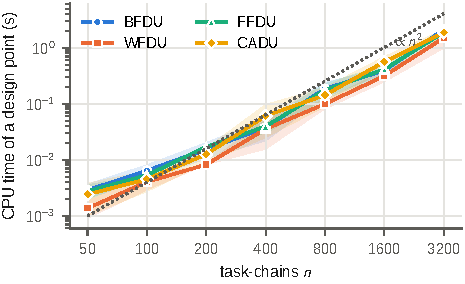
\includegraphics[width=\columnwidth]{figures/scaling}
\caption{CPU time of a design point against the number of task-chains
(log-log; dotted: slope 2).}
\label{fig:scaling}
\end{figure}

\begin{keybox}{Main findings}
\begin{itemize}[leftmargin=1em]
\item No simulated delay exceeded its bound: 3377 network flows (all four
TSN mechanisms) and 9000 task-chains simulated as a whole system, where
the end-to-end bounds are reached exactly or within 1\,\% (RQ0).
\item With consolidation, the packing rules are 2.3 to 2.9\,\% above the
optimal allocation on average, and proven optimal in 81\,\% of the
instances of up to 300 task-chains, in milliseconds; simulated annealing needs seconds to come as
close on the default platform, and a genetic algorithm does not; on the
domain platform and with slow zones, a genetic algorithm run for tens of
seconds recovers most of the gap of the packing rules, and the exact
formulation all of it (RQ1).
\item Communication awareness removes about two thirds of the inter-ECU
communications for a third more cores (RQ2).
\item ATS removes the burst growth of rings; frame replication for the
replicated task-chains costs little bandwidth and deadline satisfaction;
strict LET cuts the network bounds by 15 to 19\,\% but costs 30 points of
deadlines with \FFDU\ and 16 with \CADU\ (RQ3).
\item Memory contention can add half the cores of a packed mapping, much
less for a communication-aware one (RQ4).
\item Each core bought at the SOP buys about half a software update; the
margin after the first update is set by the design cap, not by the
provisioning (RQ6).
\item The method maps domain, hybrid and distributed platforms as well,
within 4.7\,\% of the optimum on the domain platform and 1.2\,\% on the
hybrid one (RQ1); both need about a core less than the zonal platform,
and a distributed one holds only half the applications of 300
task-chains (RQ7).
\item Consolidation saves 0.9 to 1.9 cores and the local search adds 4 to
13 points of task-chains on time; putting all free software on the
central computer costs cores, communications and 7 points on time;
whole task-chains fail under memory contention (RQ8).
\item These conclusions hold when each assumption of the generator is
set to a lower or a higher value (RQ9).
\end{itemize}
\end{keybox}

\section{Discussion}
\label{sec:discussion}

\begin{inbrief}
The experiments suggest ten design rules for an early platform.
This section states them, then the limits of the model and the threats to
the validity of the results.
\end{inbrief}

\subsection{Design rules}

\begin{enumerate}[label=\textbf{R\arabic*.}, leftmargin=2em]
\item \emph{Size the zones by their pinned work.} The zone controllers need
cores for the drivers and local task-chains wired to them. A slow
microcontroller costs cores in proportion to that work
(\cref{fig:architecture-results}); on a whole vehicle, the zones are
saturated by it.
\item \emph{Consolidate after bin packing.} Decreasing-utilization packing
is one to three cores above the optimum on small and constrained
platforms; emptying the lightest cores closes most of this gap at little
cost (\cref{fig:exact}).
\item \emph{Keep computation in the zones when they have room and timing
matters.} Communication-aware allocation trades about a third more cores
for three times fewer inter-ECU communications and fewer late
task-chains. The gain disappears when the zones are full, and the cost
shrinks when memory contention penalizes a crowded central computer.
\item \emph{Budget the backbone for the whole vehicle, not for one domain.}
At the default load the network hardly matters. At vehicle scale the link
of the central computer is the bottleneck, and a 10\,Gbit/s backbone is
worth seven points of deadline satisfaction.
\item \emph{Prefer ATS on rings and with several classes.} Asynchronous
traffic shaping removes the burst growth of cyclic topologies and keeps
the bounds of low-priority classes small; with CBS, keep LET traffic in
one class or allocate the idle slopes per port. Frame replication for the
replicated task-chains is affordable.
\item \emph{Count the contention.} When the cores of an ECU share a memory,
the cores needed grow with the cores used; a WCET measured in isolation
underestimates the platform by up to half here.
\item \emph{Provision for updates in cores, size for margin in WCETs.}
Each core bought at the SOP buys about half a software update, while the
timing margin of the platform after its first update is set by the design
cap. Sizing for a target scaling factor costs the same as an equivalent
WCET margin, but guarantees and reports it.
\item \emph{Put fast cores where the work is bound.} The same software
needs about a core less on a hybrid or a domain platform, whose ADAS (and
infotainment) controllers run part of the pinned work on big cores, than
on the zonal one; small ECUs with a fixed number of cores cannot absorb
its growth (\cref{fig:dse}).
\item \emph{Cut task-chains before they reach a core.} Most task-chains
are far below any sensible limit, but a task-chain cut only by its
bindings may no longer fit a core once the contention is counted; a limit
of half the cap kept every application feasible (\cref{tab:limit}).
\item \emph{Pay for strict LET with fewer crossings.} Strict LET makes the
data flow independent of response times and shrinks the network bounds,
but each crossing between cores waits a full producer period. Combine it
with communication-aware allocation, and set the deadlines with that wait
in mind (\cref{tab:communication}).
\end{enumerate}

\subsection{Limits of the model}

\paragraph{Platform.} The contention model is a single shared memory per
ECU with round-robin arbitration and a known number of requests per job.
Caches, interconnects with other arbitration policies, or request counts
that depend on co-runners would need a richer model, such as the
multicore response-time analysis of Davis et al.\
\cite{davis2018extensible}. Legacy buses (CAN, LIN) behind the zone
controllers are outside the network model. Each core has one LET task at
the GCD of its periods; one LET group per period would lower the overhead
on cores with fine-grained periods. Its WCET is a constant per instant,
whatever the amount of data copied, which suits short signals but not
large sensor data: a copy time that grows with the bytes copied would
make the LET load depend on the allocation.

\paragraph{Timing.} The analysis assumes synchronous releases and no
offsets, which is safe but pessimistic. The response time of
\cref{eq:rta} is valid only up to the period; a mapping with a task above
its period has no bound for that task, its task-chain or the flows it
produces, and the method treats it as unschedulable instead of analysing
the backlog \cite{lehoczky1990fixed}. LET across ECUs assumes clocks
that run at the same rate, as a synchronized time base provides
\cite{gemlau2021system}; their phases need not be aligned, since a message
waits at most one consumer period whatever the phase. Clock drift is not
modelled. The
network bounds assume a best-effort class that is always present, which is
safe again. Frame replication needs two routes without a common link or
intermediate switch: the ring and custom topologies offer them, a star or
a tree does not, and a flow without them is not replicated.
Mixed-criticality scheduling is not modelled.

\paragraph{Optimization.} The heuristic optimizes (O1) by decomposition and
(O2) by a local search that accepts only strictly improving moves and stops
at a local optimum. The exact formulation measures the gap of (O1) for
the sub-chains of the partitioning, without contention, on up to 300
task-chains on the zonal, domain and hybrid platforms, but not on the
distributed one; the optimum of (O2), and of the whole problem with
partitioning and network, remains unknown. The lifecycle analysis does not
move deployed software; allowing an update to re-allocate it would absorb
more updates, at the price of re-validating more functions.

\subsection{Threats to validity}

\emph{Construct validity.} The applications are synthetic. Their structure
(patterns, periods, tasks per pattern) is that of an industrial
engine-management software \cite{kramer2015waters}. The zone bindings,
message sizes, memory footprints, request densities and replication rates
are assumptions, and every experiment that depends on them varies them;
RQ9 varies the others, one at a time. The four platforms of RQ7 are
examples, not products.
Utilizations are relative to a reference core and scale with its speed
(the \emph{fast} case). The whole-vehicle size is an order-of-magnitude
estimate, and the updates of the lifecycle are drawn from the same
statistics as the initial software.
\emph{Internal validity.} Errors in the implementation are mitigated by
golden-result regression tests, by a randomized checker that recomputes
response times, loads, constraints and end-to-end bounds independently of
the library, by the frame-level network simulator and the full-system simulator, by
round-trip tests of the input files, and by the independent
schedulability checker of the exact formulation, whose solutions are
re-checked by the library.
\emph{External validity.} The conclusions hold for the parameter ranges
explored. The tool and the data are provided so that they can be re-run
for another platform or application.

\section{Conclusion}
\label{sec:conclusion}

Sizing a zonal E/E platform means deciding, together, where the tasks run,
how they are prioritized, how they communicate between cores at LET instants, and how their
messages cross a TSN backbone, under the wiring, memory and safety
constraints of a vehicle and for the whole life of the platform. This
paper stated that problem formally and gave a complete method to solve it.
The timing analyses come with proofs: an optimal priority assignment that
respects precedence, response times with shared-memory contention, bounds
on the maximum reaction time of multi-rate task-chains, and Network
Calculus bounds for credit-based, time-aware and asynchronous shaping and
for frame replication. The heuristic combines bin packing or a new
communication-aware rule with core consolidation, relocation moves, and a
deadline-driven local search with an exact incremental re-analysis. An exact formulation with lazy schedulability cuts shows that
the heuristic is close to optimal, and a lifecycle analysis turns the
provisioning of the hardware into a measurable trade-off with the number
of software updates the platform absorbs.

On applications built from industrial statistics, no bound was exceeded
in a frame-level simulation of the network or in a simulation of the
whole system, and the end-to-end bounds were reached, or nearly; the
packing rules with consolidation came within a few percent of the
optimal allocation in milliseconds on the default platform, where
simulated annealing needs seconds and a genetic algorithm falls behind,
while on harder platforms a genetic algorithm run for tens of seconds,
and the exact formulation, recover most of the gap; communication awareness removed
about two thirds of the inter-ECU communications at the price of a third
more cores; asynchronous traffic shaping removed the burst growth of rings;
strict LET shrank the network bounds but cost deadlines, one producer
period per crossing;
memory contention could add half the cores of a packed mapping; and each
core bought at the start of production bought about half a software
update. Consolidation and the deadline-driven local search account for
most of the benefit of the method, the conclusions hold
when the assumptions of the generator change, and the same method maps
domain, hybrid and distributed architectures, within 5\,\% of the
optimum on the domain and hybrid ones. Measuring that gap also improved
the method: it showed where free software should go on a platform
without a central computer. A whole vehicle of 2000
task-chains is mapped in about a second, so a system architect can compare
architectures, network options and provisioning policies with a
worst-case analysis behind every timing result it reports.

The natural next steps are richer contention models (caches,
interconnects), mixed-criticality scheduling, re-allocation of deployed
software during updates, and an exact treatment of the end-to-end
objective, which this paper improves but does not yet optimize.


\paragraph{Availability.} The method, the exact formulation, the
metaheuristic baselines, the two simulators and the experiments are
implemented in the open-source tool \texttt{mapping} (C11 and Python,
Apache-2.0), available at \url{https://github.com/ifupauline/mapping};
this paper and the manual are under CC BY 4.0. Its user manual,
distributed with it, describes the installation, every option, the output,
the data files, and the commands that reproduce every table and figure of
this paper.

\appendix
\section{The applications}
\label{app:generator}

\paragraph{Generator.} An application of $N$ task-chains is drawn chain by
chain from a seeded pseudo-random generator (xoshiro256** seeded by
splitmix64). The steps and their parameters are the following.
\begin{enumerate}
\item \emph{Structure} (WATERS 2015 rules \cite{kramer2015waters}): 1, 2 or
3 activation patterns with probabilities 70, 20 and 10\,\%; each pattern
has 2, 3, 4 or 5 tasks with probabilities 30, 40, 20 and 10\,\%. The
patterns of a task-chain have distinct periods, drawn with the shares of
\cref{tab:periods}.
\item \emph{Chain utilization}: log-uniform between 0.1 and 8\,\% of the
reference core; 2\,\% of the task-chains are heavy, uniform between 8 and
80\,\%.
\item \emph{Bindings}: 25\,\% of the task-chains are local to a random zone
(heavy ones never are). Of the others, 60\,\% start with a sensor task and
50\,\% end with an actuator task, each pinned to a random zone. On a
platform without zones, a random ECU that is not a central computer plays
the role of the zone. A
task-chain whose tasks would all be drivers keeps its last task free.
\item \emph{Task utilizations}: each driver takes 5\,\% of the chain
utilization; the computation tasks share the rest by UUniFast
\cite{bini2005measuring}, redrawn while a task exceeds 30\,\% of a core.
Then $C=\mathrm{round}(UT)$, at least \SI{1}{\micro s} and below $T$.
\item \emph{Messages}: 4--64 bytes (70\,\%), 65--1500 bytes (25\,\%), or
1501 bytes to 16\,kB (5\,\%).
\item \emph{Deadline}: 300\,\% of the sum of the periods of the patterns of
the task-chain, on its maximum reaction time.
\item \emph{Constraints}: memory per task log-uniform in 4--256\,KB.
Optionally, the experiments add: co-location of consecutive free tasks of
a pattern; zone-only task-chains; per-type WCET factors log-uniform in
$[(1+v)^{-1},1+v]$, lock-step equal to MCU; safety task-chains restricted to
lock-step cores; and replicas. A replica is a copy of a random non-heavy
task-chain, with its pinned tasks moved to zones that the original does
not use; the free tasks of each are kept out of the zones the other is
pinned to.
\end{enumerate}
The task-chains are finally sorted by decreasing utilization and numbered.
The task-chains of a software update (\cref{sec:lifecycle}) are drawn the
same way, from a seed derived from the seed of the application and the
number of the update, and numbered after the existing ones.

\begin{table}[ht]
\centering\small
\caption{Periods of the WATERS 2015 benchmark and their shares of the
runnables; the 15\,\% of angle-synchronous runnables are left out.}
\label{tab:periods}
\begin{tabular}{@{}lrrrrrrrrr@{}}
\toprule
period (ms) & 1 & 2 & 5 & 10 & 20 & 50 & 100 & 200 & 1000 \\
share (\%) & 3 & 2 & 2 & 25 & 25 & 3 & 20 & 1 & 4 \\
\bottomrule
\end{tabular}
\end{table}

\paragraph{The detection chain.} This illustrative ADAS chain is not taken
from a benchmark. It is one task-chain of nine tasks pinned to the central
computer, in the order GPS grabber (7/50), LIDAR grabber (12/50),
camera grabber (2/25), localization (28/50), detection (28/50), EKF
(6.5/10), fusion (25/50), planner (5/10) and control (4.5/10), where $C/T$
is in ms. The messages are 64, 16\,000, 16\,000, 256, 1024, 256, 1024, 256
and 64 bytes.

\section{The metaheuristic baselines}
\label{app:baselines}

Both baselines take the sub-chains of step 1 (\cref{sec:partitioning})
and map them onto a fixed set of \emph{candidate cores}: the initial cores
of the platform, then, for every ECU and core type, as many added cores as
the sub-chains allowed on that ECU whose lightest type it is there would
fill (their utilization on that type over $\varphi$, rounded up), within $M^{\max}_k$ and at most 64. A
mapping is admissible when it meets every constraint of
\cref{sec:problem}, schedulability included (the robust optimal priority
assignment of step 4 on every core). Both minimize the energy
\begin{equation}
E=M-\frac{0.9}{M}\sum_{p\ \text{used}}\Bigl(1-\frac{u_p}{\varphi}\Bigr)^2,
\label{eq:energy}
\end{equation}
where $M$ is the number of cores in use and $u_p$ their loads: fewer cores
first, then the free capacity gathered on few cores, the next ones to
empty. Since $E$ grows with the load, a sub-chain also prefers a
faster core. Neither runs the consolidation, and neither models
shared-memory contention. Their best mapping then gets the
deadline-driven local search of step 6, as in the heuristic, so that the
task-chains on time compare the searches. Both are deterministic for a
seed, and run on the default, slow-zone, constrained and domain
platforms of \cref{tab:exact}.

\paragraph{Simulated annealing} \cite{kirkpatrick1983optimization}. It
starts from a first fit of the sub-chains by decreasing utilization, each
to the first candidate core that takes it, the fastest cores first. A move
relocates one sub-chain to another candidate core (probability 0.7) or
exchanges two sub-chains of two cores (0.3). Half of the time, the moved
sub-chain is the one, of two drawn at random, on the less loaded core; the
target is a core in use with probability 0.8. A move that breaks a
constraint is not made, and one that raises the energy by $d$ is accepted
with probability $e^{-d/T}$, the temperature decreasing geometrically
from 0.03 to 0.0003 over the budget of moves. Every mapping visited is
admissible: a core that loses a sub-chain stays schedulable, since its
response times can only decrease.

\paragraph{Genetic algorithm.} An individual is an order of the
sub-chains, decoded by a packing heuristic, as in the hybrid genetic algorithms for
bin packing of Reeves \cite{reeves1996hybrid}. It is decoded by first fit: each sub-chain
goes to the first core in use that takes it (the fastest first, then in
the order they were opened), else opens the first candidate core that
does, the fastest first. The population has 40 individuals: the order by
decreasing utilization and random orders. Parents are chosen by binary
tournaments, recombined by order crossover (OX1, probability 0.9) and
mutated by a swap (probability 0.3); the two best individuals are kept.


\bibliographystyle{IEEEtranN}
\bibliography{refs}

\end{document}
